\documentclass[UTF8,zihao=-4]{ctexart}
\usepackage[a4paper,margin=2.45cm]{geometry}
\usepackage{amsmath,amssymb,amsthm,mathtools,bm}
\usepackage{booktabs,array}
\usepackage{graphicx}
\usepackage{tikz}
\usetikzlibrary{arrows.meta, positioning, calc}
\usepackage{subcaption}
% 面板标签 (a)(b) 置于面板上方（学术惯例：面板标签在上方，整图 caption 在下方）；
% 与图2–5 的 matplotlib 面板标题位置保持一致。
\captionsetup[subfigure]{position=top}
% 图内统一配色（流程/机制示意图共用，见 figures/*.tex）
\definecolor{flowblue}{HTML}{33475B}
\definecolor{flowfill}{HTML}{EEF3FA}
\definecolor{m0fill}{HTML}{FDEAEA}
\definecolor{m1fill}{HTML}{EAF5EA}
\definecolor{sharedred}{HTML}{C0392B}
\definecolor{winblue}{HTML}{4A90D9}
\usepackage{microtype}
\usepackage{enumitem}
\usepackage[hidelinks]{hyperref}
\usepackage{url}

\newtheorem{proposition}{命题}[section]
\theoremstyle{remark}
\newtheorem{remark}{注}[section]

\setlength{\parindent}{2em}
\setlength{\parskip}{0.25em}
\setlist{nosep,leftmargin=2.4em}

% 图件载入策略（两种模式）
%   审阅模式（默认）：本地有图件则载入原图；缺图时插入可编译占位框，便于先审阅正文与公式。
%   严格模式（strict）：缺图直接报错，CI 与发布构建必须使用——避免把"缺图"隐藏成编译成功。
%   启用方式：在 paper/ 下创建哨兵文件 STRICT.tex（CI 用 `touch paper/STRICT.tex`），
%   或改用 `xelatex -jobname=... "\def\STRICTFIGURES{}\documentclass[UTF8,zihao=-4]{ctexart}
\usepackage[a4paper,margin=2.45cm]{geometry}
\usepackage{amsmath,amssymb,amsthm,mathtools,bm}
\usepackage{booktabs,array}
\usepackage{graphicx}
\usepackage{tikz}
\usetikzlibrary{arrows.meta, positioning, calc}
\usepackage{subcaption}
% 面板标签 (a)(b) 置于面板上方（学术惯例：面板标签在上方，整图 caption 在下方）；
% 与图2–5 的 matplotlib 面板标题位置保持一致。
\captionsetup[subfigure]{position=top}
% 图内统一配色（流程/机制示意图共用，见 figures/*.tex）
\definecolor{flowblue}{HTML}{33475B}
\definecolor{flowfill}{HTML}{EEF3FA}
\definecolor{m0fill}{HTML}{FDEAEA}
\definecolor{m1fill}{HTML}{EAF5EA}
\definecolor{sharedred}{HTML}{C0392B}
\definecolor{winblue}{HTML}{4A90D9}
\usepackage{microtype}
\usepackage{enumitem}
\usepackage[hidelinks]{hyperref}
\usepackage{url}

\newtheorem{proposition}{命题}[section]
\theoremstyle{remark}
\newtheorem{remark}{注}[section]

\setlength{\parindent}{2em}
\setlength{\parskip}{0.25em}
\setlist{nosep,leftmargin=2.4em}

% 图件载入策略（两种模式）
%   审阅模式（默认）：本地有图件则载入原图；缺图时插入可编译占位框，便于先审阅正文与公式。
%   严格模式（strict）：缺图直接报错，CI 与发布构建必须使用——避免把"缺图"隐藏成编译成功。
%   启用方式：在 paper/ 下创建哨兵文件 STRICT.tex（CI 用 `touch paper/STRICT.tex`），
%   或改用 `xelatex -jobname=... "\def\STRICTFIGURES{}\documentclass[UTF8,zihao=-4]{ctexart}
\usepackage[a4paper,margin=2.45cm]{geometry}
\usepackage{amsmath,amssymb,amsthm,mathtools,bm}
\usepackage{booktabs,array}
\usepackage{graphicx}
\usepackage{tikz}
\usetikzlibrary{arrows.meta, positioning, calc}
\usepackage{subcaption}
% 面板标签 (a)(b) 置于面板上方（学术惯例：面板标签在上方，整图 caption 在下方）；
% 与图2–5 的 matplotlib 面板标题位置保持一致。
\captionsetup[subfigure]{position=top}
% 图内统一配色（流程/机制示意图共用，见 figures/*.tex）
\definecolor{flowblue}{HTML}{33475B}
\definecolor{flowfill}{HTML}{EEF3FA}
\definecolor{m0fill}{HTML}{FDEAEA}
\definecolor{m1fill}{HTML}{EAF5EA}
\definecolor{sharedred}{HTML}{C0392B}
\definecolor{winblue}{HTML}{4A90D9}
\usepackage{microtype}
\usepackage{enumitem}
\usepackage[hidelinks]{hyperref}
\usepackage{url}

\newtheorem{proposition}{命题}[section]
\theoremstyle{remark}
\newtheorem{remark}{注}[section]

\setlength{\parindent}{2em}
\setlength{\parskip}{0.25em}
\setlist{nosep,leftmargin=2.4em}

% 图件载入策略（两种模式）
%   审阅模式（默认）：本地有图件则载入原图；缺图时插入可编译占位框，便于先审阅正文与公式。
%   严格模式（strict）：缺图直接报错，CI 与发布构建必须使用——避免把"缺图"隐藏成编译成功。
%   启用方式：在 paper/ 下创建哨兵文件 STRICT.tex（CI 用 `touch paper/STRICT.tex`），
%   或改用 `xelatex -jobname=... "\def\STRICTFIGURES{}\documentclass[UTF8,zihao=-4]{ctexart}
\usepackage[a4paper,margin=2.45cm]{geometry}
\usepackage{amsmath,amssymb,amsthm,mathtools,bm}
\usepackage{booktabs,array}
\usepackage{graphicx}
\usepackage{tikz}
\usetikzlibrary{arrows.meta, positioning, calc}
\usepackage{subcaption}
% 面板标签 (a)(b) 置于面板上方（学术惯例：面板标签在上方，整图 caption 在下方）；
% 与图2–5 的 matplotlib 面板标题位置保持一致。
\captionsetup[subfigure]{position=top}
% 图内统一配色（流程/机制示意图共用，见 figures/*.tex）
\definecolor{flowblue}{HTML}{33475B}
\definecolor{flowfill}{HTML}{EEF3FA}
\definecolor{m0fill}{HTML}{FDEAEA}
\definecolor{m1fill}{HTML}{EAF5EA}
\definecolor{sharedred}{HTML}{C0392B}
\definecolor{winblue}{HTML}{4A90D9}
\usepackage{microtype}
\usepackage{enumitem}
\usepackage[hidelinks]{hyperref}
\usepackage{url}

\newtheorem{proposition}{命题}[section]
\theoremstyle{remark}
\newtheorem{remark}{注}[section]

\setlength{\parindent}{2em}
\setlength{\parskip}{0.25em}
\setlist{nosep,leftmargin=2.4em}

% 图件载入策略（两种模式）
%   审阅模式（默认）：本地有图件则载入原图；缺图时插入可编译占位框，便于先审阅正文与公式。
%   严格模式（strict）：缺图直接报错，CI 与发布构建必须使用——避免把"缺图"隐藏成编译成功。
%   启用方式：在 paper/ 下创建哨兵文件 STRICT.tex（CI 用 `touch paper/STRICT.tex`），
%   或改用 `xelatex -jobname=... "\def\STRICTFIGURES{}\input{main}"`。
\newif\ifstrictfigures
\strictfiguresfalse
\IfFileExists{STRICT.tex}{\strictfigurestrue}{}

\let\OriginalIncludeGraphics\includegraphics
\RenewDocumentCommand{\includegraphics}{O{} m}{%
  \IfFileExists{#2}{%
    \OriginalIncludeGraphics[#1]{#2}%
  }{%
    \ifstrictfigures
      \PackageError{owtda-paper}{Strict build: missing figure `\detokenize{#2}'}%
        {The strict build (paper/STRICT.tex present) requires every figure to exist.}%
    \else
      \begin{minipage}[c][4.2cm][c]{0.82\linewidth}
        \centering\small 图件缺失：\texttt{\detokenize{#2}}
      \end{minipage}%
    \fi
  }%
}

\title{重叠窗口拓扑扫描的有限样本校准边界\\\large Finite-Sample Calibration Boundaries for Topological Change-Point Scans with Overlapping Windows}
\author{
  王平\textsuperscript{1}\quad
  黄盛南\textsuperscript{1}\quad
  张晓媛\textsuperscript{1,*}\\[2mm]
  \small $^1$河北金融学院统计与数据科学学院\\[1mm]
  \small 通讯作者：张晓媛，\texttt{zxy0407010229@163.com}
}
\date{2026年9月}

\begin{document}
\maketitle

\begin{abstract}
\input{sections/00_abstract}
\end{abstract}

\section*{Abstract}
\input{sections/00_abstract_en}

\input{sections/01_intro}
\input{sections/02_method}
\input{sections/03_theory}
\input{sections/04_protocol}
\input{sections/05_h0}
\input{sections/06_h1}
\input{sections/07_real}
\input{sections/08_discussion}
\input{sections/09_conclusion}

\section*{Data and Code Availability}
复现本文结果的代码、配置、种子清单、完整逐格数据与补充材料由仓库 \url{https://github.com/dw0911/owtda-calibration} 提供。本稿对应 git 标签 \texttt{v1.1.1-paper}；全部合成数据均由该版本代码与固定随机种子生成，不依赖外部数据归档，独立数据 DOI 尚在建立中，未作为已提供材料列出。补充材料 S5 给出代码入口与复现步骤。

\bibliographystyle{unsrt}
\bibliography{bibliography}
\end{document}
"`。
\newif\ifstrictfigures
\strictfiguresfalse
\IfFileExists{STRICT.tex}{\strictfigurestrue}{}

\let\OriginalIncludeGraphics\includegraphics
\RenewDocumentCommand{\includegraphics}{O{} m}{%
  \IfFileExists{#2}{%
    \OriginalIncludeGraphics[#1]{#2}%
  }{%
    \ifstrictfigures
      \PackageError{owtda-paper}{Strict build: missing figure `\detokenize{#2}'}%
        {The strict build (paper/STRICT.tex present) requires every figure to exist.}%
    \else
      \begin{minipage}[c][4.2cm][c]{0.82\linewidth}
        \centering\small 图件缺失：\texttt{\detokenize{#2}}
      \end{minipage}%
    \fi
  }%
}

\title{重叠窗口拓扑扫描的有限样本校准边界\\\large Finite-Sample Calibration Boundaries for Topological Change-Point Scans with Overlapping Windows}
\author{
  王平\textsuperscript{1}\quad
  黄盛南\textsuperscript{1}\quad
  张晓媛\textsuperscript{1,*}\\[2mm]
  \small $^1$河北金融学院统计与数据科学学院\\[1mm]
  \small 通讯作者：张晓媛，\texttt{zxy0407010229@163.com}
}
\date{2026年9月}

\begin{document}
\maketitle

\begin{abstract}
基于持续同调的时间序列变点检验可利用滑动窗口提取局部结构特征，但窗口共享观测引起的依赖可能使随机置换参考分布失真。本文考察固定持续图向量表示与最大扫描所构成检验的有限样本校准。首先，以高斯窗口均值构造反例，说明原始观测独立同分布仍不足以保证派生窗口序列的交换性。随后，在固定窗口数与固定原始观测长度两种设计下，对 28 个零假设配置比较无约束窗口级随机置换与依赖乘子自助法，并以均值--协方差特征作为非拓扑对照。在名义显著性水平 0.05 下，对每种表示，20 个重叠配置均表现为实质反保守，持续同调表示的经验拒绝率最高为 0.9756。依赖乘子法在全部匹配配置中降低拒绝率，但对每种表示，8 个非重叠配置均表现为实质保守；原序列依赖对步长对比的修饰方向随生成过程与表示变化。低阶矩匹配的圆形到 8 字形曲线备择下，两类表示的尺寸校正功效分别为 1.0000 和 0.0620；整体平移负对照则呈相反结果，与距离型持续同调的平移不变性一致。结果表明，当前实现的校准表现具有明确的条件依赖性，降低拒绝率不能等同于恢复名义校准，表示的信号敏感性与检验的误报控制应分别评价。

\noindent\textbf{关键词}：持续同调；变点检测；重叠滑动窗口；交换性；有限样本校准。

\end{abstract}

\section*{Abstract}
Change-point tests based on persistent homology use sliding windows to extract local structural features, but dependence induced by shared observations can distort random-permutation reference distributions. This study examines the finite-sample calibration of a test combining a fixed vector representation of persistence diagrams with a maximum scan statistic. A Gaussian window-mean counterexample first shows that independent and identically distributed raw observations do not ensure exchangeability of the derived window sequence. Naive unrestricted window-level permutation and a dependent multiplier bootstrap are then evaluated under fixed-window-count and fixed-observation-length designs across 28 null configurations, with mean--covariance features as a non-topological comparator. At the nominal level of 0.05, all 20 overlapping-window configurations are classified as materially anti-conservative for each representation; the empirical rejection rate for the persistent-homology representation reaches 0.9756. The multiplier procedure lowers rejection rates in every matched configuration, but all eight non-overlapping configurations are materially conservative for each representation. The effect of serial dependence on the stride contrast varies across generators and representations. Under a circle-to-figure-eight alternative with matched first and second marginal moments, size-adjusted powers are 1.0000 and 0.0620 for the persistent-homology and moment representations, respectively. A mean-shift negative control reverses this ordering, consistently with the translation invariance of distance-based persistent homology. These results demonstrate condition-dependent calibration for the studied implementation: lower rejection rates do not necessarily imply nominal calibration, and representation sensitivity and Type-I error control require separate evaluation.

\noindent\textbf{Keywords}: persistent homology; change-point detection; overlapping sliding windows; exchangeability; finite-sample calibration.


\section{引言}\label{sec:intro}

\subsection{研究背景与统计问题}\label{sec:intro-bg}

时间序列的结构变化既可能表现为均值、方差等低阶统计量的改变，也可能表现为局部轨迹几何、周期结构或状态空间形状的改变。滑动窗口和时延嵌入为后一类信号提供了局部化表示：每个时间片段被转换为点云，持续同调进一步从多尺度上提取连通分支和环等结构信息。相关理论奠定了滑动窗口持久性分析的基础\cite{PereaHarer2015}，持续图像等有限维表示则使持续图能够进入统计扫描和机器学习程序\cite{Adams2017}。近年来，拓扑摘要已被用于离线变点检测、在线监测及依赖序列中的结构异常识别\cite{IslambekovYuvarajGel2020,ZhengMakXieXie2023,ChazalLevrardRoyer2024,NieYue2026}。

为提高候选变点的扫描密度，实际分析常取步长 $s$ 小于窗口宽度 $W$。此时，相邻窗口共享原始观测，窗口特征序列由此形成局部依赖。设第 $i$ 个窗口经固定映射得到特征 $Y_i$。对全部窗口顺序实施置换时，有限样本精确性通常依赖联合分布对排列群保持不变，即
\begin{equation}\label{eq:intro-exchangeability}
 (Y_1,\ldots,Y_M)\overset{d}{=}(Y_{\pi(1)},\ldots,Y_{\pi(M)}),
 \qquad \forall\,\pi\in\mathfrak S_M.
\end{equation}
独立同分布是满足该条件的一种充分情形，排列操作直接要求的条件则是窗口特征层面的联合交换性。窗口共享观测可诱发局部依赖，但特定映射是否具有交换性取决于其联合分布；平稳性、边际同分布以及原始序列的独立同分布性质，在窗口重叠时均不足以一般性地推出式\eqref{eq:intro-exchangeability}。由此形成本文关注的统计错配：科学零假设定义在原始过程的“无变化”层面，置换校准所需的对称性定义在派生窗口特征的联合分布层面。依赖时间序列中的置换理论同样表明，未经修正的排列参考分布可能无法维持名义检验水平\cite{RomanoTirlea2022}；随机排列检验的有限样本有效性还需相应的群不变性条件\cite{HemerikGoeman2018}。

本文考察一种基于持续同调特征的变点检验：每个局部时间窗口映射为点云，点云经持续同调及固定向量化形成特征序列，再通过标准化部分和的最大值检测前后特征均值差异。持续同调决定检验保留的结构信息，重采样程序决定统计量的参考分布。本文重点评价窗口重叠对后者有限样本校准的影响，并以均值--协方差特征作为非拓扑对照。

\subsection{相关工作与研究缺口}\label{sec:intro-lit}

与本文相关的研究可概括为三条脉络。第一类工作研究滑动窗口嵌入、持续同调及持续图向量化，为局部时间片段的拓扑表示提供方法基础\cite{PereaHarer2015,Adams2017}，其关注点主要在于表示的稳定性与可解释性，而未系统考察重叠窗口下推断有效性的有限样本校准。第二类工作将拓扑摘要引入离线或在线变化检测，并显式处理时间依赖与误报控制：文献\cite{NieYue2026}已经分析重叠窗口下的依赖继承，并利用移动块自助法校准在线监测控制限；其它近邻工作则聚焦表示对结构变化的辨识能力及特定检测程序的性能\cite{IslambekovYuvarajGel2020,ZhengMakXieXie2023,ChazalLevrardRoyer2024}。本文沿用这一研究背景，固定表示、离线最大扫描和校准规则，比较两种观测预算下的零假设拒绝率与经验分类。第三类工作研究依赖数据下的置换、dependent wild bootstrap 与依赖乘子自助法，说明时间依赖会改变随机化参考分布，并为若干均值、光滑函数或经验过程问题建立渐近理论\cite{RomanoTirlea2022,Shao2010,BucherKojadinovic2016}。这些理论为窗口特征序列提供了渐近分析的起点，但其适用性仍需针对本文所用的局部映射、扫描泛函与带宽规则逐项验证。

这些结果尚未提供本文实现的具体有限样本保证：重叠局部窗口依次经过点云映射、持续同调向量化和最大扫描后，朴素置换会产生多大程度的有限样本尺寸失真；该失真如何随重叠程度、原序列依赖、观测预算和表示类型变化；依赖感知校准能够在哪些条件下减弱失真，又会在哪些条件下表现为保守或残留反保守。本文不以非线性变换本身主张该管线脱离既有理论框架，也不从渐近一致性推定当前样本规模下的名义尺寸控制，而以固定实现和预设设计网格上的有限样本校准偏差及其条件变化为考察重点。本文将条件组合 $\theta$ 下的有效检验水平记为 $\alpha_{\mathrm{eff}}(\theta)$，并将映射 $\theta\mapsto\alpha_{\mathrm{eff}}(\theta)$ 称为预设离散设计网格上的条件化有限样本校准图谱。本文不估计连续参数空间中的解析边界；“经验校准状态转换”仅指有序设计维度（主要为步长或重叠率）上相邻格点发生校准分类变化的位置。该图谱属于有限样本、点态和设计域内的刻画，不提供全参数空间的统一保证。

\subsection{研究目标与贡献}\label{sec:intro-contrib}

本文的主要贡献是对固定持续同调变点检验开展条件化有限样本校准评价：在两种预算设计和 28 个唯一零假设配置上，报告朴素置换与依赖乘子的拒绝率、区间及经验分类，并量化两种预算下重叠与非重叠条件之间的预设对比。机制分析通过一般局部映射的依赖继承和窗口均值反例说明交换性风险；备择分析通过低阶矩匹配的形状构造与整体平移负对照，解释固定表示的信号敏感性及不变性。理论推导、经验评价与构造对照分别承担机制、实际表现和解释功能。

全文其余部分安排如下：第~\ref{sec:method} 节定义重叠窗口特征、两类表示、最大扫描统计量及校准方法；第~\ref{sec:theory} 节分析有限依赖、交换性失效与方差机制；第~\ref{sec:protocol} 节说明评价对象和实验设计；第~\ref{sec:h0} 节报告零假设下的有限样本校准结果；第~\ref{sec:h1} 节分析备择下的检出与定位性能；第~\ref{sec:discussion} 节讨论方法含义、适用范围与局限；第~\ref{sec:conclusion} 节总结全文。

\section{基于持续同调特征的变点检验}\label{sec:method}

图~\ref{fig:flow}给出整体流程与统计冲突的来源：窗口是随机化单位，但重叠使原始观测被多个随机化单位共享。后续小节依次定义窗口构造、两种表示、最大扫描统计量与两种校准方法。

\begin{figure}[tbp]
\centering
\begin{subfigure}[t]{0.92\linewidth}
\centering
\caption{统计推断主流程}\label{fig:flow-a}
\input{figures/fig1_flow}
\end{subfigure}

\vspace{1.2em}

\begin{subfigure}[t]{0.85\linewidth}
\centering
\caption{窗口重叠与共享观测机制}\label{fig:flow-b}
\input{figures/fig1_overlap}
\end{subfigure}

\caption{基于持续同调特征的变点检验与校准流程。(a) 原始序列经重叠窗口映射为窗口点云，再分别经持续同调—向量化分支得到 BPI、经均值—协方差分支得到矩表示 MOMENTS，进入最大扫描得到检验统计量 $T_M$ 与位置估计 $\hat k$；随后 M0 无约束窗口级随机置换重采样、M1 相关乘子重采样分别构造参考分布，并通过 Monte Carlo $p$ 值形成拒绝决策。(b) 重叠机制：相邻窗口共享原始观测（红色），无约束窗口级随机置换重排窗口顺序时原有邻接被破坏，这是后文交换性失效机制的直观来源。}\label{fig:flow}
\end{figure}

\subsection{窗口构造与局部点云}\label{sec:windows}

给定观测序列 $X_1,\ldots,X_T$，取窗口宽度 $W$ 和步长 $s$，并令
\begin{equation}\label{eq:windows}
 a_i=(i-1)s+1,\qquad
 I_i=\{a_i,\ldots,a_i+W-1\},\qquad
 M=\left\lfloor\frac{T-W}{s}\right\rfloor+1.
\end{equation}
本文考虑 $1\le s\le W$，相邻窗口的名义重叠率为 $1-s/W$。对于二维观测，窗口点云直接定义为 $P_i=\{X_t:t\in I_i\}$。对于标量观测，在每个窗口内部构造三维时延点云
\begin{equation}\label{eq:delay-cloud}
 P_i=\bigl\{(X_t,X_{t+3},X_{t+6}):t=a_i,\ldots,a_i+W-7\bigr\},
\end{equation}
因而时延坐标不会跨越窗口边界。点云在计算持续同调前按固定规则进行精确去重；所有坐标尺度、网格、核宽和截断参数均预先设定，且不利用整条序列共同估计的自适应参数。该局部性条件将在第~\ref{sec:theory} 节用于界定窗口特征的依赖范围。

\subsection{固定网格持续强度表示}\label{sec:bpi}

对每个点云 $P_i$，在系数域 $\mathbb F_2$ 上按欧氏距离计算 Vietoris--Rips 持续同调，并保留 0 维和 1 维同调通道中有限且寿命为正的 birth--death 对。过滤采用边长阈值的直径约定：单形 $\sigma$ 的过滤值为其顶点间最大欧氏距离，即 $\operatorname{diam}(\sigma)$；尺度 $\varepsilon$ 下纳入所有满足 $\operatorname{diam}(\sigma)\le\varepsilon$ 的单形，即 $\operatorname{VR}_\varepsilon(P)=\{\sigma\subseteq P:\operatorname{diam}(\sigma)\le\varepsilon\}$。过滤不设数据驱动的截断上限，持续图坐标直接以欧氏距离尺度报告。由于有限欧氏点云的 Vietoris--Rips 过滤在过滤值达到点云直径时形成完全复形，所有 1 维同调类在此时均已消亡，仅最后一个 0 维连通分量的 death 为 $\infty$；实现中只丢弃该显式无限 death 分量，其余有限类全部保留。相关计算框架和有限维表示可分别参见\cite{Bauer2021,Adams2017}。

记 $K_i(\varepsilon)=\operatorname{VR}_\varepsilon(P_i)$。随过滤尺度 $\varepsilon$ 增大，复形形成嵌套序列 $K_i(\varepsilon)\subseteq K_i(\varepsilon')$（$\varepsilon\le\varepsilon'$）。零维同调记录连通分支，一维同调记录未被二维单形填充的独立循环；贝蒂数 $\beta_q(K_i(\varepsilon))=\dim H_q(K_i(\varepsilon);\mathbb F_2)$ 表示该尺度下相应同调空间的维数。持续同调进一步记录这些类随过滤尺度的出现与消失，由持续图中的 $(b,d)$ 概括，其中 $b$ 与 $d$ 分别为出生尺度与消亡尺度，$d-b$ 是过滤尺度上的寿命，而非真实时间轴上的持续时长。记第 $q\in\{0,1\}$ 个同调通道的持续图为
\[
 \mathcal D_i^{(q)}=\{(b_{ij}^{(q)},d_{ij}^{(q)})\}_j.
\]
给定场景固定的尺度上界 $c$，将每个有限持续图点转换为归一化 birth--lifetime 坐标。尺度上界 $c$ 仅用于该坐标缩放与截断，不用于提前终止过滤；过滤本身以 $+\infty$ 为阈值完整计算。
\begin{equation}\label{eq:bpi-normalization}
 u_{ij}^{(q)}=\min\left(\frac{b_{ij}^{(q)}}{c},1\right),\qquad
 v_{ij}^{(q)}=\min\left(\frac{d_{ij}^{(q)}-b_{ij}^{(q)}}{c},1\right).
\end{equation}
令 $\Delta=1/20$、$g_r=(r+1/2)\Delta$（$r=0,\ldots,19$）以及 $\sigma=0.05$。第 $q$ 个通道在网格中心 $(g_r,g_\ell)$ 上的持续强度坐标定义为
\begin{equation}\label{eq:bpi}
 Z_{i,r\ell}^{(q)}
 =\frac{\Delta}{2\pi\sigma^2}
 \sum_j v_{ij}^{(q)}
 \exp\left\{-\frac{(g_r-u_{ij}^{(q)})^2+(g_\ell-v_{ij}^{(q)})^2}{2\sigma^2}\right\}.
\end{equation}
每个同调通道产生 $20\times20=400$ 个坐标。按 0 维、1 维同调通道的顺序向量化并连接，再除以 $\sqrt 2$（该缩放使两个同调通道对总平方距离的贡献取等权平均），得到 800 维特征。此处涉及三类维数：同调维数 $q\in\{0,1\}$、点云所在空间维数 $d\in\{2,3\}$ 以及向量表示维数 $p=800$；$800$ 维特征不意味着本文研究了 $800$ 维拓扑。
\begin{equation}\label{eq:bpi-vector}
 Y_i^{\mathrm{BPI}}
 =\frac{1}{\sqrt2}
 \begin{bmatrix}
   \operatorname{vec}(Z_i^{(0)})\\
   \operatorname{vec}(Z_i^{(1)})
 \end{bmatrix}.
\end{equation}
空通道记为 400 维零向量。N-AR 时延点云取 $c=6$，圆形模型及其备择取 $c=2.5$。本文将每个持续图中以寿命加权的高斯核表面在固定网格中心进行评价，并将两个同调通道的结果拼接为向量，沿用实现标识 BPI。该表示与持续图像共享“持续图--加权核表面--有限维表示”的思路，但其离散化采用网格中心采样，区别于逐像素积分\cite{Adams2017}。BPI 仅标识本文的固定实现，不另行宣称一种标准 Betti 不变量，也不构成对随机持续图总体强度密度的估计\cite{WuKimRinaldo2023}。

\subsection{矩表示}\label{sec:moments}

为构造低阶统计摘要作为对照，设窗口点云为 $P_i=\{x_{ij}\}_{j=1}^{n_i}\subset\mathbb R^d$，并定义
\begin{equation}\label{eq:moments}
 \bar x_i=\frac1{n_i}\sum_{j=1}^{n_i}x_{ij},\qquad
 S_i=\frac1{n_i}\sum_{j=1}^{n_i}(x_{ij}-\bar x_i)(x_{ij}-\bar x_i)^\top.
\end{equation}
MOMENTS 特征依次连接均值、协方差对角元以及按固定字典序排列的 $\sqrt2(S_i)_{ab}$（$a<b$）：
\begin{equation}\label{eq:moments-vector}
 Y_i^{\mathrm{MOM}}
 =\bigl(\bar x_i^\top,(S_i)_{11},\ldots,(S_i)_{dd},
 \{\sqrt2(S_i)_{ab}:a<b\}\bigr)^\top.
\end{equation}
其维数为 $d(d+3)/2$，故二维和三维点云分别得到 5 维和 9 维特征。$\sqrt2$ 权重保证任意两个窗口 $i,j$ 满足
\begin{equation}\label{eq:moments-frob}
 \|Y_i^{\mathrm{MOM}}-Y_j^{\mathrm{MOM}}\|_2^2
 =\|\bar x_i-\bar x_j\|_2^2+\|S_i-S_j\|_F^2.
\end{equation}
该表示主要概括一、二阶矩；有限窗口和序列依赖仍可能使其响应某些形状变化，因此本文不预设其对所有拓扑变化均不敏感。

\subsection{最大扫描统计量与位置估计}\label{sec:scan}

本文采用的最大扫描统计量属于变点分析中标准化部分和型统计量的常见构造\cite{CsorgoHorvath1997}。对任一窗口特征序列 $Y_1,\ldots,Y_M\in\mathbb R^p$，令
\begin{equation}\label{eq:bridge}
 U_M(k)=\frac1{\sqrt M}
 \left(\sum_{i=1}^kY_i-\frac{k}{M}\sum_{i=1}^M Y_i\right),
 \qquad t_k=\frac{k}{M},
\end{equation}
并定义标准化扫描曲线与最大统计量
\begin{equation}\label{eq:scan}
 Q_M(k)=\frac{\|U_M(k)\|_2^2}{t_k(1-t_k)},\qquad
 T_M=\max_{k\in\mathcal K_M}Q_M(k),
\end{equation}
其中
\[
 \mathcal K_M=\{\lceil0.15M\rceil,\ldots,M-\lceil0.15M\rceil\},
\]
比例 $0.15$ 为确认性分析前固定的边界保护比例，用于避免左右片段过短。
等价地，若 $\bar Y_{1:k}$ 和 $\bar Y_{k+1:M}$ 分别表示左右两段样本均值，则
\begin{equation}\label{eq:scan-equivalent}
 Q_M(k)=\frac{k(M-k)}{M}
 \|\bar Y_{1:k}-\bar Y_{k+1:M}\|_2^2.
\end{equation}
因此，该扫描统计量直接响应左右两段窗口特征的均值之差，检验对象是特征均值层面的变化；它不构成对任意原始分布或任意拓扑变化都具有一致检出能力的通用检验。

对 BPI 表示，令 $V_i^{(q)}=\operatorname{vec}(Z_i^{(q)})$ 为第 $q$ 个同调通道的未缩放向量，并分别对每个通道使用相同的桥接与标准化，得到 $Q_M^{(q)}(k)$。由 $Y_i^{\mathrm{BPI}}=\frac1{\sqrt2}[V_i^{(0)};V_i^{(1)}]$ 及平方欧氏范数的线性性，对每个候选位置 $k$ 有
\[
 Q_M^{\mathrm{BPI}}(k)=\frac12 Q_M^{(0)}(k)+\frac12 Q_M^{(1)}(k).
\]
因此总扫描同时受连通分支持续信息与循环持续信息影响。由于最大值的位置通常不同，$\max_k\tfrac12\bigl(Q_M^{(0)}(k)+Q_M^{(1)}(k)\bigr)$ 一般不等于两个通道最大值的平均 $\tfrac12\max_k Q_M^{(0)}(k)+\tfrac12\max_k Q_M^{(1)}(k)$。本文实验将两个同调通道合并报告，未单独分离零维与一维同调的贡献。

为使浮点并列情形具有确定性，令 $\epsilon_{64}=2^{-52}$，将满足
\[
 Q_M(k)\ge T_M-64\epsilon_{64}\max(1,|T_M|)
\]
的连续候选段定义为合格平台。位置估计选取最长平台；长度并列时取最左平台，再以该平台的下中位数作为 $\widehat k$。由于 $k$ 表示第 $k$ 与第 $k+1$ 个窗口之间的分割，映射到原始时间轴后的连续边界估计为
\begin{equation}\label{eq:location-map}
 \widehat\tau=\left(\widehat k-\frac12\right)s+\frac{W+1}{2}.
\end{equation}
该映射将第 $\widehat k$ 与第 $\widehat k+1$ 个窗口之间的分割点对应到二者中心之间的中点。若特征序列精确恒定，则规定 $T_M=0$。所有校准方法均使用相同的观测统计量、候选集合和位置规则。

\subsection{校准方法}\label{sec:calibration}

朴素置换方法记为 M0。M0 从排列群 $\mathfrak S_M$ 上的均匀分布中独立抽取随机排列；下文称为全局随机置换，以区别于块置换或局部置换。条件于观测到的窗口特征，M0 对每个随机排列序列重新计算式\eqref{eq:scan}。该方法保留经验边际分布，却不保留原始窗口顺序中的局部依赖。

依赖乘子自助法记为 M1。令 $\bar Y=M^{-1}\sum_{i=1}^M Y_i$、$Z_i=Y_i-\bar Y$，并取
\begin{equation}\label{eq:dmb-bandwidth}
 b=\max\left\{\left\lfloor\frac Ws\right\rfloor+1,
                 \left\lceil M^{1/3}\right\rceil\right\}.
\end{equation}
乘子新息 $\varepsilon_1,\ldots,\varepsilon_{M+b-1}$ 为独立标准正态，由与观测样本分离的随机流生成，因而与观测样本相互独立；不同内层重复使用各自的随机流独立生成。定义
\begin{equation}\label{eq:dmb-multiplier}
 \xi_i=b^{-1/2}\sum_{j=0}^{b-1}\varepsilon_{i+j},
 \qquad i=1,\ldots,M.
\end{equation}
由此
\begin{equation}\label{eq:dmb-cov}
 \operatorname{Cov}(\xi_i,\xi_{i+h})
 =\left(1-\frac{|h|}{b}\right)_+.
\end{equation}
M1 不作循环回绕，并对乘子加权序列 $\{\xi_iZ_i\}_{i=1}^M$ 应用与观测样本相同的桥接扫描。该构造属于依赖感知的参考近似；dependent wild bootstrap 和依赖乘子过程的一般理论可参见\cite{Shao2010,BucherKojadinovic2016}，其结论不直接构成本文完整 BPI 最大扫描的有限样本有效性定理。

两种方法均使用 $B=999$ 次重采样。若
\[
 K=\sum_{r=1}^{B}\mathbf 1\{T_{M,r}^*\ge T_M\},
\]
则 Monte Carlo $p$ 值定义为
\begin{equation}\label{eq:mc-pvalue}
 p=\frac{K+1}{B+1}=\frac{K+1}{1000}.
\end{equation}
本文以 $p\le0.05$ 拒绝零假设，等价于 $K\le49$。加一形式避免有限重采样下报告零 $p$ 值\cite{PhipsonSmyth2010}，但不恢复重叠窗口的交换性，也不替代对 M1 参考近似有效性的评估；随机排列检验的有限样本有效性仍需相应的群不变性条件\cite{HemerikGoeman2018}。

\section{重叠窗口的交换性与方差机制}\label{sec:theory}

本节利用可解析的窗口均值构造说明重叠如何改变派生统计量的联合分布。对随机向量 $(Y_1,\ldots,Y_M)$，若对任意排列 $\pi\in\mathfrak S_M$ 都有
\[
 (Y_1,\ldots,Y_M)\overset d=(Y_{\pi(1)},\ldots,Y_{\pi(M)}),
\]
则称其具有交换性。以下结果依次讨论局部映射的依赖范围、交换性反例、有限样本方差以及排列参考与原始顺序之间的协方差差异。相关结论用于解释失校准机制，不直接给出一般拓扑最大扫描的误报率公式。

\subsection{窗口局部映射的依赖范围}\label{sec:t1}

固定局部窗口映射的依赖继承是后续机制分析的基础，相关结果已见文献\cite{NieYue2026}（附录命题 6）。为明确本文的窗口与映射条件，下面给出原始观测独立同分布情形的自包含证明。

\begin{proposition}[局部映射的有限依赖范围]\label{prop:dependency}
设原始观测 $\{X_t\}$ 独立同分布，且
\[
 Y_i=\Psi\bigl((X_t)_{t\in I_i}\bigr),
\]
其中 $\Psi$ 为固定可测映射，并且不使用由整条序列共同估计的参数。则 $\{Y_i\}$ 至多为
\[
 m=\left\lceil\frac Ws\right\rceil-1
\]
阶依赖序列。
\end{proposition}

\begin{proof}
取任意两个窗口指标集合 $A,B\subset\{1,\ldots,M\}$，并假设 $\min_{i\in A,j\in B}|i-j|>m$。对任意 $i\in A$ 与 $j\in B$，不妨设 $i<j$，则
$$(j-i)s\ge\left\lceil W/s\right\rceil s\ge W,$$
从而 $I_i\cap I_j=\varnothing$。因此，$\{X_t:t\in\cup_{i\in A}I_i\}$ 与 $\{X_t:t\in\cup_{j\in B}I_j\}$ 生成的两个 $\sigma$-代数相互独立，其固定可测函数 $\{Y_i:i\in A\}$ 与 $\{Y_j:j\in B\}$ 也相互独立。由 $m$-依赖的定义即得结论。
\end{proof}

命题~\ref{prop:dependency}给出依赖范围的上界。窗口发生重叠时，具体协方差是否为零仍取决于原始分布和映射 $\Psi$；局部依赖也不自动等同于不可交换性，后者需要考察完整联合分布。

\subsection{交换性失效的精确反例}\label{sec:t2}

\begin{proposition}[高斯窗口均值的非交换性]\label{prop:counterexample}
设 $X_t\overset{\mathrm{iid}}{\sim}N(0,\sigma^2)$，其中 $\sigma^2>0$；设 $1\le s<W$ 且窗口数 $M\ge3$。记 $(x)_+=\max(x,0)$。令
\[
 Z_i=\frac1W\sum_{t\in I_i}X_t.
\]
则对 $h=0,\ldots,M-1$ 及 $i=1,\ldots,M-h$，
\begin{equation}\label{eq:window-cov}
 \Gamma_h=\operatorname{Cov}(Z_i,Z_{i+h})
 =\frac{\sigma^2}{W^2}(W-hs)_+,
\end{equation}
且随机向量 $(Z_1,\ldots,Z_M)$ 不具交换性。
\end{proposition}

\begin{proof}
由于原始观测相互独立，只有两个窗口共享的观测指标对协方差有贡献。交集 $I_i\cap I_{i+h}$ 含有 $(W-hs)_+$ 个指标，故得到式\eqref{eq:window-cov}。又因 $1\le s<W$，有
\[
 \Gamma_1=\frac{\sigma^2}{W^2}(W-s)
 >\frac{\sigma^2}{W^2}(W-2s)_+=\Gamma_2.
\]
考虑交换第 2、3 个坐标的排列。交换前，第一坐标与第二、第三坐标的协方差分别为 $\Gamma_1$ 和 $\Gamma_2$；交换后两者互换。协方差矩阵由此发生改变。高斯向量的分布由均值和协方差矩阵唯一确定，因此交换后的联合分布与原分布不同。
\end{proof}

\begin{remark}
该反例说明，原始观测的独立同分布性质不足以保证重叠窗口统计量具有交换性。结论并未覆盖所有固定局部映射，例如常数映射始终产生可交换序列。条件 $M\ge3$ 也具有实质作用：当 $M=2$ 时，两个等方差的联合高斯窗口均值具有对称协方差矩阵，交换两个坐标不会改变其分布。
\end{remark}

\subsection{窗口均值的有限样本方差比}\label{sec:t3}

\begin{proposition}[窗口均值的精确方差比]\label{prop:variance}
在命题~\ref{prop:counterexample}的构造下，令
\[
 \bar Z_M=\frac1M\sum_{i=1}^M Z_i,
 \qquad \Gamma_0=\frac{\sigma^2}{W}.
\]
则
\begin{align}
 \operatorname{Var}(\bar Z_M)
 &=\frac{\Gamma_0}{M}A_{\mathrm{mean},M},\label{eq:mean-var}\\
 A_{\mathrm{mean},M}
 &=1+2\sum_{h=1}^{M-1}
 \left(1-\frac hM\right)
 \left(1-\frac{hs}{W}\right)_+.
 \label{eq:finite-vif-general}
\end{align}
若 $W=qs$、$q$ 为正整数且 $M\ge q$，则
\begin{equation}\label{eq:finite-vif}
 A_{\mathrm{mean},M}=q-\frac{q^2-1}{3M}.
\end{equation}
\end{proposition}

\begin{proof}
按滞后展开协方差和，
\[
 M^2\operatorname{Var}(\bar Z_M)
 =M\Gamma_0+2\sum_{h=1}^{M-1}(M-h)\Gamma_h.
\]
将式\eqref{eq:window-cov}代入并除以 $M^2$，即可得到式\eqref{eq:mean-var}--\eqref{eq:finite-vif-general}。当 $W=qs$ 且 $M\ge q$ 时，非零求和项仅为 $h=1,\ldots,q-1$。利用
\[
 \sum_{h=1}^{q-1}\left(1-\frac hq\right)=\frac{q-1}{2},
 \qquad
 \sum_{h=1}^{q-1}h\left(1-\frac hq\right)=\frac{q^2-1}{6},
\]
整理后得到式\eqref{eq:finite-vif}。
\end{proof}

在本文的一个主要几何配置 $W=64$、$s=16$、$M=192$ 下，$q=4$，故
\[
 A_{\mathrm{mean},M}=4-\frac{15}{576}\approx3.974.
\]
该数值描述标量窗口均值相对于独立窗口基准的方差比。BPI 最大扫描还受到高维方向、特征谱和极值操作影响，因此不能将 $3.974$ 解释为其 I 类错误率的膨胀倍数。

\subsection{长期协方差与排列参考的错配}\label{sec:t4}

当 $W=qs$ 时，标量窗口均值为 $(q-1)$-依赖序列，其长期方差为
\begin{equation}\label{eq:long-run-var}
 \Omega
 =\sum_{h=-\infty}^{\infty}\Gamma_h
 =\Gamma_0+2\sum_{h=1}^{q-1}\Gamma_h
 =q\Gamma_0.
\end{equation}
只要 $q>1$，就有 $\Omega>\Gamma_0$。原始顺序下的部分和变异包含滞后协方差，随机排列参考则主要由窗口值的经验边际变异决定。

这一差别可由有限总体恒等式进一步说明。给定 $z_1,\ldots,z_M$，令
\[
 \bar z=\frac1M\sum_{i=1}^M z_i,
 \qquad
 s_M^2=\frac1M\sum_{i=1}^M(z_i-\bar z)^2,
\]
并令 $\pi$ 为 $\{1,\ldots,M\}$ 上的均匀随机排列。对 $1\le k<M$，
\begin{equation}\label{eq:permutation-fpc}
 \operatorname{Var}_{\pi}\left[
 \frac1{\sqrt M}\sum_{i=1}^k(z_{\pi(i)}-\bar z)
 \,\middle|\,z_1,\ldots,z_M\right]
 =\frac{k(M-k)}{M(M-1)}s_M^2.
\end{equation}
式\eqref{eq:permutation-fpc}源于不放回抽样中不同抽取位置的条件协方差 $-s_M^2/(M-1)$。因此，排列桥接过程的条件变异由经验边际量 $s_M^2$ 决定，而原始窗口顺序还携带式\eqref{eq:long-run-var}所概括的滞后依赖。该机制与依赖时间序列中置换有效性需要附加条件的结论一致\cite{RomanoTirlea2022}。

协方差结构的差异为失校准提供了机制解释。对于一般多维非线性特征，协方差矩阵不相等本身仍不足以推出最大扫描统计量的极限分布必然不同；同样，重叠率增加也不保证每一种表示或校准器的 I 类错误率单调变化。

上述结果证明，窗口重叠能够破坏窗口级随机化所需的联合对称条件，并揭示全局随机置换遗漏原顺序滞后协方差的机制；但这些解析结果没有给出 BPI 最大扫描的有限样本误报率闭式表达。因此，第~\ref{sec:h0} 节通过预设设计网格上的 Monte Carlo 实验评估完整非线性管线的实际有限样本校准。

\section{实验设计与评价规约}\label{sec:protocol}

\subsection{评价对象与操作性定义}\label{sec:estimands}\label{sec:rq}

令
\[
 \theta=(g,\rho,s,r,\varphi,\mathcal C)
\]
表示一个完整的零假设条件，其中 $g$ 为数据生成过程，$\rho$ 为原序列依赖参数，$s$ 为窗口步长，$r\in\{\mathrm{fixed}\text{-}M,\mathrm{fixed}\text{-}T\}$ 为预算制度，$\varphi\in\{\mathrm{BPI},\mathrm{MOMENTS}\}$ 为表示，$\mathcal C\in\{\mathrm{M0},\mathrm{M1}\}$ 为校准方法。名义显著性水平固定为 $\alpha=0.05$。本文的有效检验水平指配置条件下的零假设拒绝概率，并以 Monte Carlo 经验 I 类错误率估计；它不构成对整个零假设族取上确界的复合检验 size。该配置条件下的拒绝概率定义为
\begin{equation}\label{eq:effective-size}
 \alpha_{\mathrm{eff}}(\theta)
 =\Pr_{H_0,\theta}\{p_\theta\le0.05\}.
\end{equation}
映射 $\theta\mapsto\alpha_{\mathrm{eff}}(\theta)$ 构成本文的有限样本校准图谱（“图谱”仅指预设设计网格上的拒绝概率及经验分类，不指估计了连续响应面）。本文所称经验校准状态转换，是预设设计网格中有序设计维度（主要为步长或重叠率）上相邻格点发生校准分类变化的位置。

每个零假设配置均报告拒绝率及无连续性修正的 Wilson 区间\cite{Wilson1927}。预先冻结的实用等价带为
\[
 \mathcal E=[0.035,0.065].
\]
逐格分类规则如下：90\% Wilson 区间完整包含于 $\mathcal E$ 时，记为点态实用校准；95\% Wilson 区间上界低于 $0.035$ 时，记为实质保守；95\% Wilson 区间下界高于 $0.065$ 时，记为实质反保守；其余情形记为未定（未满足任一分类判据，不代表参数恰好位于真实边界）。该分类属于点态判断，不构成设计域上的同时概率保证。

备择实验考察两个相互关联的对象：其一，使用匹配零假设经验临界值计算的尺寸校正功效，用于比较表示所保留的信号信息；其二，基于观测扫描曲线得到的定位误差和“检出且定位成功”的联合概率。相应定义见第~\ref{sec:alternatives} 节和第~\ref{sec:h1-localization} 节。

\subsection{零假设数据生成过程}\label{sec:dgp}

首先生成平稳高斯 AR(1) 过程
\begin{equation}\label{eq:latent-ar}
 G_t=\rho G_{t-1}+\sqrt{1-\rho^2}\,\varepsilon_t,
 \qquad
 G_0\sim N(0,1),\quad
 \varepsilon_t\overset{\mathrm{iid}}{\sim}N(0,1),
\end{equation}
其中 $G_0$ 与全部新息相互独立，$\rho\in\{0,0.8\}$。实现中舍弃最初 1000 个值；由于初值取自平稳分布，该步骤作为统一的生成约定保留。

N-AR 直接取标量观测
\begin{equation}\label{eq:n-ar}
 X_t=G_t.
\end{equation}
N-CIRCLE 先以标准正态分布函数 $\Phi$ 作概率积分变换，再映射到单位圆：
\begin{equation}\label{eq:n-circle}
 U_t=\Phi(G_t),\qquad
 C(u)=(\cos 2\pi u,\sin 2\pi u),\qquad
 X_t=C(U_t)+0.08\eta_t,
\end{equation}
其中 $\eta_t\overset{\mathrm{iid}}{\sim}N_2(0,I_2)$，并与潜变量过程独立。对每个固定 $t$，$U_t$ 服从 $U(0,1)$；当 $\rho=0$ 时，两类原始过程均为独立同分布序列，当 $\rho=0.8$ 时则保留时间依赖。N-CIRCLE 的定义基于平稳高斯过程的边际变换，不涉及随机游走或增量过程。两个数据生成过程覆盖两类典型观测形态：N-AR 为标量序列，须经时延嵌入形成点云，对应一维时间序列场景；N-CIRCLE 为二维序列，窗口点云直接进入持续同调，对应多维观测场景。其潜在无噪声曲线具有圆形几何；加入观测噪声后，含噪观测分布的严格支撑为整个 $\mathbb R^2$，但有限点云在所考察过滤尺度上仍呈现明显的环状持续结构，便于考察拓扑表示对循环结构变化的敏感性。依赖水平取 $\rho\in\{0,0.8\}$，分别对应独立同分布与较强时间依赖两种端点情形，用于检验交换性失效对原序列依赖程度的敏感性。

\subsection{双预算制度}\label{sec:budget}

窗口宽度在确认性分析前固定为 $W=64$；本文不对该取值的最优性作主张。步长取
\[
 s\in\{8,16,32,64\},
\]
对应名义重叠率 $1-s/W$ 依次为 $87.5\%$、$75\%$、$50\%$ 与 $0$，覆盖从高重叠到无重叠的梯度，用于刻画重叠程度对校准的影响。
本文采用两种互补的预算制度：
\begin{itemize}
\item \textbf{固定窗口数（fixed-$M$）}：令 $M=192$，并由 $T=W+s(M-1)$ 确定原始序列长度；对应的 $T$ 依次为 $1592$、$3120$、$6176$ 和 $12288$。
\item \textbf{固定观测长度（fixed-$T$）}：令 $T=3120$，并由式\eqref{eq:windows}确定窗口数；对应的 $M$ 依次为 $383$、$192$、$96$ 和 $48$。
\end{itemize}
固定窗口数制度保持扫描器接收的特征数量不变，固定观测长度制度保持原始数据预算不变。两种制度在 $s=16$ 时共享相同的 $(T,M)=(3120,192)$ 几何配置；共享配置按同一逻辑实验单元计数。因此，$2$ 个数据生成过程、$2$ 个依赖水平和两种预算制度最终形成 28 个唯一零假设配置。

表~\ref{tab:design}给出两种预算制度下的完整窗口几何。该表同时说明：7 个唯一窗口几何的来源；两种制度在 $s=16$ 处的共享；$T$ 与 $M$ 如何随制度和步长变化；以及 M1 依赖乘子带宽为何随配置改变。

\input{../artifacts/tables/Table1_design.tex}


图~\ref{fig:alternatives}展示两类备择构造的几何形态。

\begin{figure}[ht]
\centering
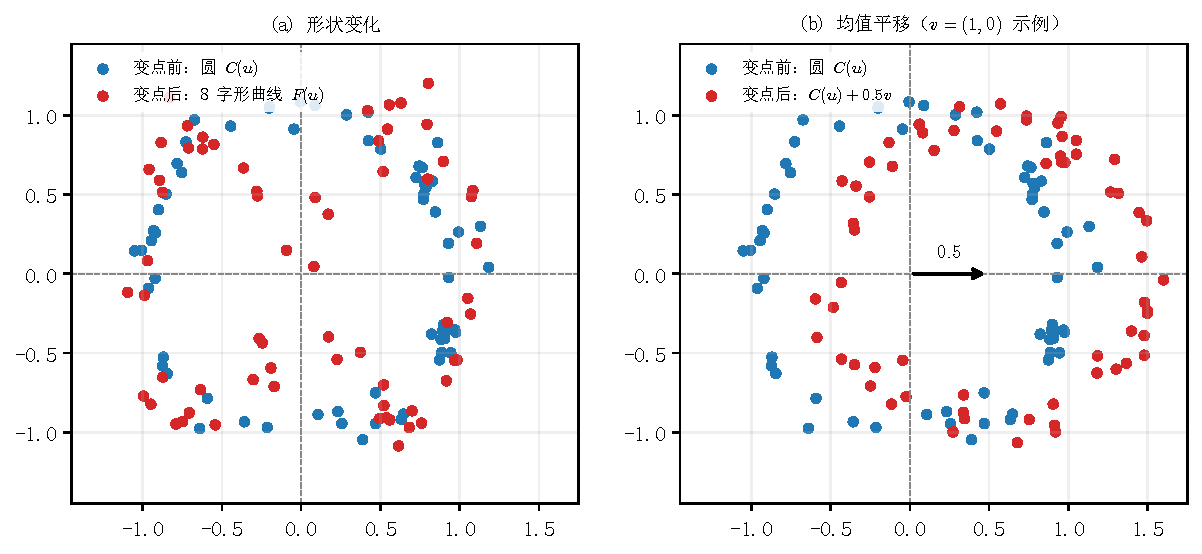
\includegraphics[width=0.95\textwidth]{../artifacts/figures/Figure2_alternative_geometry.pdf}
\caption{两类备择构造。(a) 形状变化：变点前为圆 $C(U_t)=(\cos2\pi U_t,\sin2\pi U_t)$，变点后改为 8 字形曲线 $F(U_t)=(\sin2\pi U_t,\sin4\pi U_t)$；(b) 均值平移：变点后整体平移 $+0.5v$，图中 $v=(1,0)$ 为示例方向，正式实验中 $v$ 跨重复随机、重复内固定。散点为含观测噪声 $0.08\eta_t$ 的 64 个点；圆与 8 字形曲线仅匹配单时点均值与协方差，完整滞后联合分布未被声明为相同。两个场景分别针对 BPI 与 MOMENTS 的结构敏感性。}\label{fig:alternatives}
\end{figure}

\subsection{Monte Carlo 设置}\label{sec:mc}

每格内部 $R_0=2500$（零假设）或 $R_1=1600$（备择）次主重复相互独立；不同格之间按主重复编号保留配对结构。每次方法校准均使用 $B=999$ 次内层重采样，并按式\eqref{eq:mc-pvalue}计算 $p$ 值。零假设部分包含
\[
 28\times2\text{（表示）}\times2\text{（方法）}\times2500
 =280{,}000
\]
条方法--表示评价记录；备择部分包含
\[
 2\text{（场景）}\times4\text{（条件）}\times2\text{（表示）}
 \times2\text{（方法）}\times1600
 =51{,}200
\]
条记录。外层 Monte Carlo 因而同时包含数据生成随机性与 $B=999$ 次内层校准的有限重采样随机性。

\subsection{预先设定的主对比}\label{sec:primary}

令 $\pi_{g,\rho,s,m}^{(r)}$ 表示在 BPI 表示、预算制度 $r$ 和校准方法 $m\in\{\mathrm{M0},\mathrm{M1}\}$ 下的零假设拒绝概率，且 $g\in\mathcal G=\{\mathrm{N\mbox{-}AR},\mathrm{N\mbox{-}CIRCLE}\}$。三个主对比均在确认性分析前冻结：
\begin{align}
\mathrm{P1}:\quad & D_{\mathrm{OV}}^{M}
 =\frac12\sum_{g\in\mathcal G}
 \left(\pi_{g,0,16,\mathrm{M0}}^{(M)}
      -\pi_{g,0,64,\mathrm{M0}}^{(M)}\right),
 \label{eq:p1}\\
\mathrm{P2}:\quad & D_{\mathrm{ST}}^{T}
 =\frac12\sum_{g\in\mathcal G}
 \left(\pi_{g,0,16,\mathrm{M0}}^{(T)}
      -\pi_{g,0,64,\mathrm{M0}}^{(T)}\right),
 \label{eq:p2}\\
\mathrm{P3}:\quad & D_{\mathrm{CONS}}
 =0.05-\frac12\sum_{g\in\mathcal G}
 \pi_{g,0,64,\mathrm{M1}}^{(M)}.
 \label{eq:p3}
\end{align}
P1 与 P2 检验单侧假设 $D\le0.10$ 对 $D>0.10$；P3 检验 $D_{\mathrm{CONS}}\le0.01$ 对 $D_{\mathrm{CONS}}>0.01$。阈值 $0.10$ 与 $0.01$ 均为查看确认性结果前规定的最小实质差异：$0.10$ 对应两个数据生成过程等权平均下至少 10 个百分点的 I 类错误率差异，$0.01$ 对应相对于名义水平 $0.05$ 至少 1 个百分点的保守偏差。MOMENTS 的同构对比仅作次级描述，不进入主要多重性族。

主对比使用 10,000 次按数据生成过程分层的整簇自助法。同一主重复编号下的全部相关条件、表示和方法随簇共同重采样，以保留配对结构。对一般效应量 $\widehat\theta$ 及单侧阈值 $\theta_0$，自助 $p$ 值定义为
\begin{equation}\label{eq:bootstrap-p}
 p_{\mathrm{boot}}
 =\frac{1+\sum_{b=1}^{10000}
 \mathbf1\{\widehat\theta_b^*-\widehat\theta
 \ge \widehat\theta-\theta_0\}}
 {10001}.
\end{equation}
因此，自助 $p$ 值不可能等于零。若 $q_\gamma$ 表示 10,000 个自助估计的最近秩（nearest-rank）$\gamma$ 分位数，则边际 95\% 基本型自助区间（basic bootstrap interval）\cite{DavisonHinkley1997}为
\begin{equation}\label{eq:basic-ci}
 \left[2\widehat\theta-q_{0.975},\,
       2\widehat\theta-q_{0.025}\right],
 \qquad
 q_\gamma=\widehat\theta^*_{(\lceil10000\gamma\rceil)}.
\end{equation}
三个单侧 $p$ 值采用 Holm step-down 校正\cite{Holm1979}，族水平为 $0.05$。本文将校正后 $p\le0.05$ 作为预先设定的操作性支持标准，同时用式\eqref{eq:basic-ci}报告效应量不确定性；该区间为边际区间，不解释为 Holm 同时置信区间。

\subsection{备择构造与尺寸校正功效}\label{sec:alternatives}

备择实验以 N-CIRCLE 为基础，并在完整序列上连续生成同一潜变量过程和观测噪声，不在变点处重置随机状态。令
\[
 \tau=\left\lfloor\frac T2\right\rfloor,
 \qquad
 F(u)=(\sin2\pi u,\sin4\pi u).
\]
形状变化场景定义为
\begin{equation}\label{eq:shape-alt}
 X_t=
 \begin{cases}
 C(U_t)+0.08\eta_t, & t\le\tau,\\
 F(U_t)+0.08\eta_t, & t>\tau.
 \end{cases}
\end{equation}
当 $U_t\sim U(0,1)$ 时，$C(U_t)$ 与 $F(U_t)$ 的单时点均值均为零，协方差均为 $I_2/2$；加入同分布噪声后，这两个单时点边际矩仍保持匹配。该构造不要求变点前后的完整滞后联合分布或二阶过程相同。

该备择旨在改变潜在几何中的独立循环结构，同时匹配单时点一、二阶矩：无噪声圆 $C([0,1])$ 同胚于 $S^1$，8 字形曲线 $F([0,1])$ 同胚于 $S^1\vee S^1$，二者在 $\mathbb F_2$ 系数下的一阶 Betti 数分别为 $1$ 和 $2$。但这一事实属于潜在连续曲线；有限含噪点云经 Vietoris--Rips 过滤后的持续图取决于抽样、噪声与尺度，不能被保证恰好分别产生一条与两条长寿命条带。本文实际检验的对象仍是有限点云持续图向量的均值变化。

均值平移场景定义为
\begin{equation}\label{eq:mean-alt}
 X_t=C(U_t)+0.08\eta_t+0.5v\mathbf1\{t>\tau\},
 \qquad
 v=(\cos2\pi V,\sin2\pi V),\quad V\sim U(0,1),
\end{equation}
其中方向变量 $V\sim U(0,1)$ 由独立随机流生成，与潜变量过程、观测噪声相互独立；每次 Monte Carlo 重复抽取一个方向 $v$，并在该重复内固定。每个备择场景均使用 $M=192$、$s\in\{16,64\}$ 和 $\rho\in\{0,0.8\}$，共四个条件。

尺寸校正功效使用与备择条件、表示和几何配置匹配的零假设观测统计量。将 $R_0=2500$ 个零假设统计量按升序记为
\[
 T_{M,(1)}^{H_0}\le\cdots\le T_{M,(R_0)}^{H_0},
\]
并令
\begin{equation}\label{eq:h0-critical}
 j_{0.95}=\left\lceil0.95(R_0+1)\right\rceil=2376,
 \qquad
 \widehat c_{0.95}^{H_0}=T_{M,(2376)}^{H_0}.
\end{equation}
对备择统计量 $T_{M,r}^{H_1}$，定义
\begin{equation}\label{eq:size-adjusted-power}
 \widehat\beta_{\mathrm{std}}
 =\frac1{R_1}\sum_{r=1}^{R_1}
 \mathbf1\{T_{M,r}^{H_1}>\widehat c_{0.95}^{H_0}\}.
\end{equation}
由于 M0 与 M1 共享同一观测统计量，式\eqref{eq:size-adjusted-power}在每个“条件--表示”组合上只计算一次，用于评价表示敏感性，不用于排列两种校准方法的优劣。

场景层面的表示差 $\Delta$ 通过两层整簇自助法估计。重采样单位为主复制（cluster）：零假设层按 N-CIRCLE 主复制整簇重采样以重算经验临界值，备择层按备择主复制整簇重采样以重算功效；共进行 2000 个联合 bootstrap 重复，每次分别独立重采样 H0 簇和 H1 簇，并产生一个场景差值。BPI 与 MOMENTS 使用同一重采样索引成对移动，四个 $(\rho,s)$ 条件在每个场景内先计算各自的 BPI 减 MOMENTS 功效差，再等权平均得到场景差。区间采用最近秩法（nearest-rank）定义的 2000 次百分位区间（$2.5\%$ 与 $97.5\%$ 分位数）。

\subsection{可复现性说明}\label{sec:repro}

实验协议、随机种子、配置和主要分析规则均在查看正式结果前确定。零假设与备择结果来自不可变的正式试次记录，正文数值由统一汇总文件生成。代码、环境文件、规范化结果和完整逐格输出由冻结的软件 release 提供，其地址见文末 Data and Code Availability。

\section{零假设下的有限样本校准结果}\label{sec:h0}

本节报告 28 个唯一零假设配置下，朴素置换（M0）与依赖乘子自助法（M1）的有限样本 I 类错误率。分析重点为条件化校准图谱及其逐格边界，汇总均值仅作为辅助描述。

\subsection{双预算制度下的校准图谱}\label{sec:h0-heatmap}

图~\ref{fig:m0-surface} 给出 M0 在两种预算制度下的 I 类错误率表面，图~\ref{fig:m1-deviation} 给出 M1 的校准偏差 $\widehat\alpha-0.05$。两幅图均为 $2\times2$ 分面：行区分数据生成过程，列区分固定窗口数与固定观测长度，面板内纵轴保留 $\rho$ 与步长两个条件维度。两图共有 16 个“条件--表示--方法”数值因共享几何 $s=16$、$T=3120$、$M=192$ 而被有意重复展示，用于分别解释两种预算制度，不应视为两份独立证据。完整 $16\times4$ 热图见补充材料 S4。

\begin{figure}[ht]
\centering
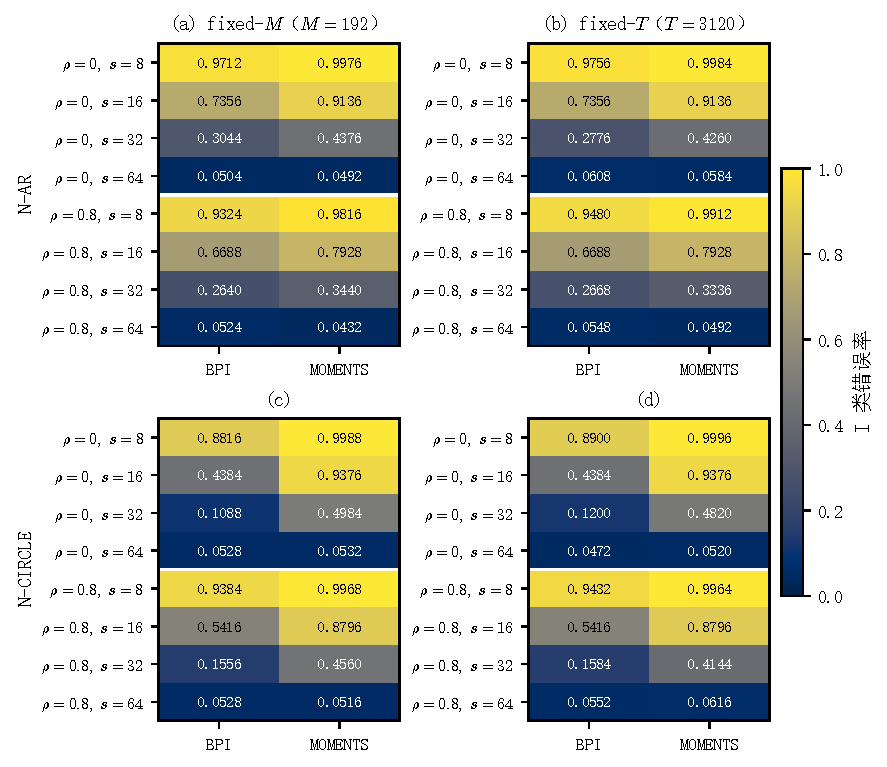
\includegraphics[width=0.92\textwidth]{../artifacts/figures/Figure3_M0_type1_surface.pdf}
\caption{M0（朴素置换）在两种预算制度下的有限样本 I 类错误率表面。两行分别为 N-AR 与 N-CIRCLE 数据生成过程，两列分别为固定窗口数（$M=192$）与固定观测长度（$T=3120$）；每面板行按 $\rho\times s$（$\rho\in\{0,0.8\}$，$s\in\{8,16,32,64\}$）排列，列为 BPI 与 MOMENTS 表示。色标 $[0,1]$，格内标注四位小数拒绝率。}\label{fig:m0-surface}
\end{figure}

\begin{figure}[ht]
\centering
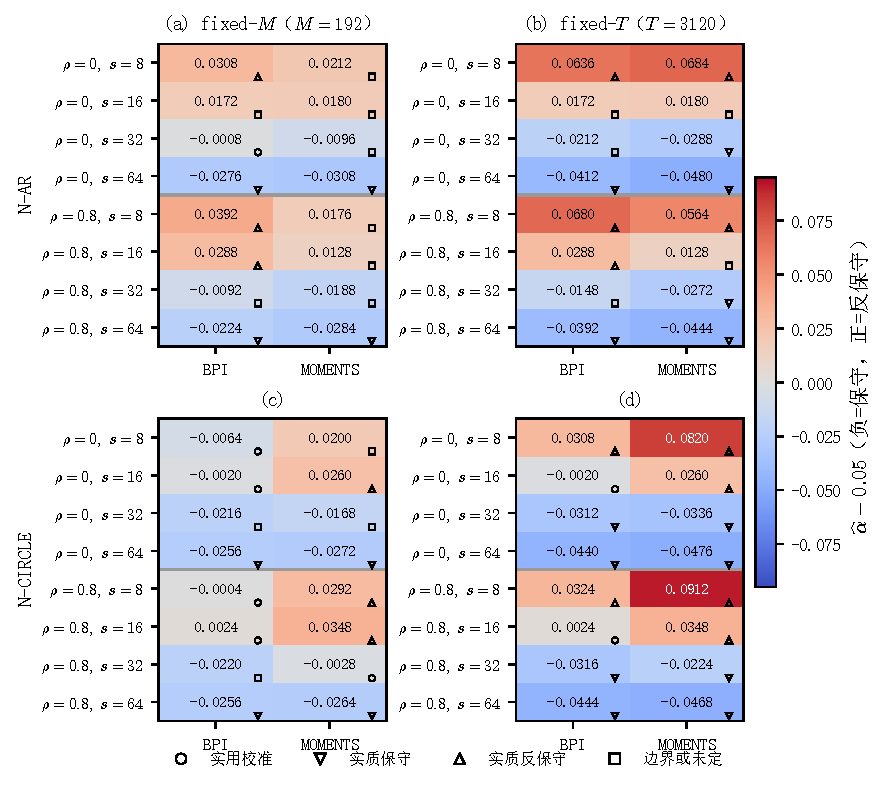
\includegraphics[width=0.92\textwidth]{../artifacts/figures/Figure4_M1_deviation_surface.pdf}
\caption{M1（依赖乘子法）在两种预算制度下的校准偏差 $\widehat\alpha-0.05$。两行分别为 N-AR 与 N-CIRCLE 数据生成过程，两列分别为固定窗口数与固定观测长度；每面板行按 $\rho\times s$（$\rho\in\{0,0.8\}$，$s\in\{8,16,32,64\}$）排列，列为 BPI 与 MOMENTS。色尺关于 0 对称，格内标注四位小数偏差；符号编码逐格 Wilson 判定（置于单元格右上角）：圆圈=实用校准，下三角=实质保守，上三角=实质反保守，方块=边界或未定。}\label{fig:m1-deviation}
\end{figure}

M0 的校准表现对窗口重叠高度敏感。BPI/M0 的逐格拒绝率介于 $0.0472$ 和 $0.9756$ 之间，MOMENTS/M0 介于 $0.0432$ 和 $0.9996$ 之间；对两种表示，20 个唯一重叠配置的 M0 均被判为实质反保守。M1 明显压缩了极端反保守性，其对应范围分别为 $0.0056$--$0.1180$ 和 $0.0020$--$0.1412$；对两种表示，8 个唯一非重叠配置的 M1 均被判为实质保守。在全部 56 个匹配的“配置--表示”组合中，M1 的拒绝率均低于 M0，但更低的拒绝率并不等同于更准确的校准。M1 的拒绝率同时分布在名义水平以下和以上，表明依赖感知乘子改变了校准图谱的形态，却未在所有有限样本配置中实现统一校准。

上述范围也说明，单一总体平均会掩盖具有相反方向的局部偏差。某些配置中的保守性和另一些配置中的反保守性可以在汇总后相互抵消，因此本文以逐格有效尺寸作为主要报告单位。

\subsection{逐格校准分类}\label{sec:h0-classify}

共有
\[
 28\text{（零假设配置）}\times2\text{（表示）}\times2\text{（方法）}=112
\]
个逐格评价单元。依据第~\ref{sec:estimands} 节的预设规则，表~\ref{tab:calibration}汇总四类校准状态。

\input{../artifacts/tables/Table4_calibration.tex}


对两种表示，M0 均有 $20/28$ 个配置被判为实质反保守，且没有配置被判为实质保守。M1 的分类则分散于实用校准、实质保守、实质反保守和边界未定四类：BPI/M1 中四类计数依次为 $5$、$10$、$7$ 和 $6$，MOMENTS/M1 中依次为 $1$、$12$、$7$ 和 $8$。这些计数描述预设设计网格内的有限样本分布，不应解释为方法在更广参数空间中的“通过率”。

\subsection{相邻格点的经验校准边界}\label{sec:h0-boundary}

题名中的“经验校准边界”对应有序设计维度上相邻格点发生校准状态变化的位置。以固定窗口数、N-AR、$\rho=0$、BPI 为例，依据逐格拒绝计数及第~\ref{sec:estimands} 节的 Wilson 判据，逐格状态随步长变化如下：$s=8,16,32$ 时 M0 均被判为实质反保守，$s=64$ 时转为实用校准，故 M0 的观测分类在步长 $32$ 与 $64$ 之间发生转换；M1 则随步长增加依次经历实质反保守（$s=8$）、边界或未定（$s=16$）、实用校准（$s=32$）与实质保守（$s=64$）。这里报告的是相邻格点的观测状态变化，不估计两点之间的连续临界步长，也不将其解释为连续参数域上的置信区间。完整的状态转换清单见补充材料 S1。

\subsection{主对比 P1--P3}\label{sec:h0-primary}

表~\ref{tab:primary}报告三个预先冻结主对比的点估计、边际 95\% basic 自助区间和 Holm 校正结果。按照第~\ref{sec:primary} 节的单侧阈值与多重性规则，三项对比均满足预设支持标准。

\input{../artifacts/tables/Table3_primary_contrasts.tex}


在固定窗口数制度下，$s=16$ 相对于 $s=64$ 的 M0 拒绝率差异，经两个数据生成过程等权平均后为 $0.5354$；在固定观测长度制度下，相应差异为 $0.5330$。两项区间的下界均远高于预设阈值 $0.10$，相对于该阈值的超额分别为 $0.4354$ 和 $0.4330$。因此，在两个预设数据生成过程、$\rho=0$ 和 BPI 表示的等权平均意义下，P1 与 P2 在各自预算制度下均超过预设的 $0.10$ 实质阈值，并通过 Holm 校正后的单侧判定。该结论不延伸为每一数据生成过程、每一依赖水平或每一表示下的必然规律。

P3 的估计为 $0.0266$，其 95\% 区间完整高于预设阈值 $0.01$。这表明在 $\rho=0$、$s=W=64$、固定 $M=192$ 的非重叠端，当前 M1 配置表现出可检测的保守偏差。该结果同时提示，依赖感知校准器在窗口不重叠时也需要接受有限样本验证。

\subsection{原序列依赖的效应修饰}\label{sec:h0-rho}

为避免将单一步长下的 $\rho$ 差异与重叠效应修饰混为一谈，次级分析采用步长对比的差。对数据生成过程 $g$、表示 $\varphi$ 和预算制度 $r$，定义
\begin{align}
 D_{g,\varphi}^{(r)}(\rho)
 &=\pi_{g,\rho,16,\mathrm{M0},\varphi}^{(r)}
  -\pi_{g,\rho,64,\mathrm{M0},\varphi}^{(r)},\\
 I_{g,\varphi}^{(r)}
 &=D_{g,\varphi}^{(r)}(0.8)-D_{g,\varphi}^{(r)}(0).
 \label{eq:rho-interaction}
\end{align}
其中 $I_{g,\varphi}^{(r)}$ 衡量原序列依赖对“$s=16$ 相对于 $s=64$”拒绝率差异的修饰。

描述性估计汇总于表~\ref{tab:rho-interaction}。正值表示 $\rho=0.8$ 放大步长对比，负值表示其缩小步长对比；修饰方向随数据生成过程和表示而变化，且不同条件的符号并不一致。由于该分析为次级描述，本文不据此提出原序列依赖具有统一单调作用的结论。

\begin{table}[ht]
\centering
\caption{原序列依赖对步长对比（$s=16$ 相对 $s=64$）的效应修饰 $I_{g,\varphi}^{(r)}$。正值表示 $\rho=0.8$ 放大步长对比，负值表示其缩小步长对比。}\label{tab:rho-interaction}
\begin{tabular}{llcc}
\toprule
表示 & 数据生成过程 & $I^{(M)}$ & $I^{(T)}$\\
\midrule
BPI & N-AR & $-0.0688$ & $-0.0608$\\
BPI & N-CIRCLE & $0.1032$ & $0.0952$\\
MOMENTS & N-AR & $-0.1148$ & $-0.1116$\\
MOMENTS & N-CIRCLE & $-0.0564$ & $-0.0676$\\
\bottomrule
\end{tabular}
\end{table}

\section{表示特异性的检出与定位性能}\label{sec:h1}

本节考察两类方向相反的备择。尺寸标准化功效按式\eqref{eq:size-standardized-power}计算：每个备择条件和表示均使用对应零假设配置的经验 0.95 临界值，从而减少参考分布松紧对表示比较的直接干扰。由于 M0 与 M1 使用相同的观测扫描统计量，每个“条件--表示”组合只产生一个尺寸标准化功效。场景层面的功效为四个预设条件 $(\rho,s)\in\{0,0.8\}\times\{16,64\}$ 的等权平均。

\subsection{形状变化}\label{sec:h1-shape}

在圆形到八字曲线的形状变化下，两种表示的平均尺寸标准化功效分别为
\[
 \widehat\beta_{\mathrm{BPI}}=1.00000,
 \qquad
 \widehat\beta_{\mathrm{MOMENTS}}=0.06203.
\]
定义场景差异为 BPI 减去 MOMENTS，则
\begin{equation}\label{eq:shape-power-diff}
 \Delta_{\mathrm{shape}}=0.93797,
 \qquad
 \text{95\% CI }[0.92969,0.94609].
\end{equation}
该区间为 2000 次保持条件配对结构的重采样所得 95\% 百分位自助区间。结果表明，在当前形状构造和固定表示参数下，BPI 保留了 MOMENTS 的一、二阶摘要未充分捕获的结构信息。该证据的适用范围限于本文定义的备择、窗口几何和表示实现，不能推广为拓扑表示对任意变化类型均占优势。

\subsection{均值平移反向对照}\label{sec:h1-mean}

在均值平移场景下，BPI 的平均尺寸标准化功效为 $0.05375$，MOMENTS 为 $1.00000$，因此
\begin{equation}\label{eq:mean-power-diff}
 \Delta_{\mathrm{mean}}=-0.94625,
 \qquad
 \text{95\% CI }[-0.95344,-0.93844].
\end{equation}
差异方向与形状变化场景相反。MOMENTS 直接包含窗口均值，因而在该构造中具有很高的检出能力；BPI 的尺寸标准化功效接近名义水平，说明固定持续强度表示对该平移信号的敏感性有限。

\begin{figure}[ht]
\centering
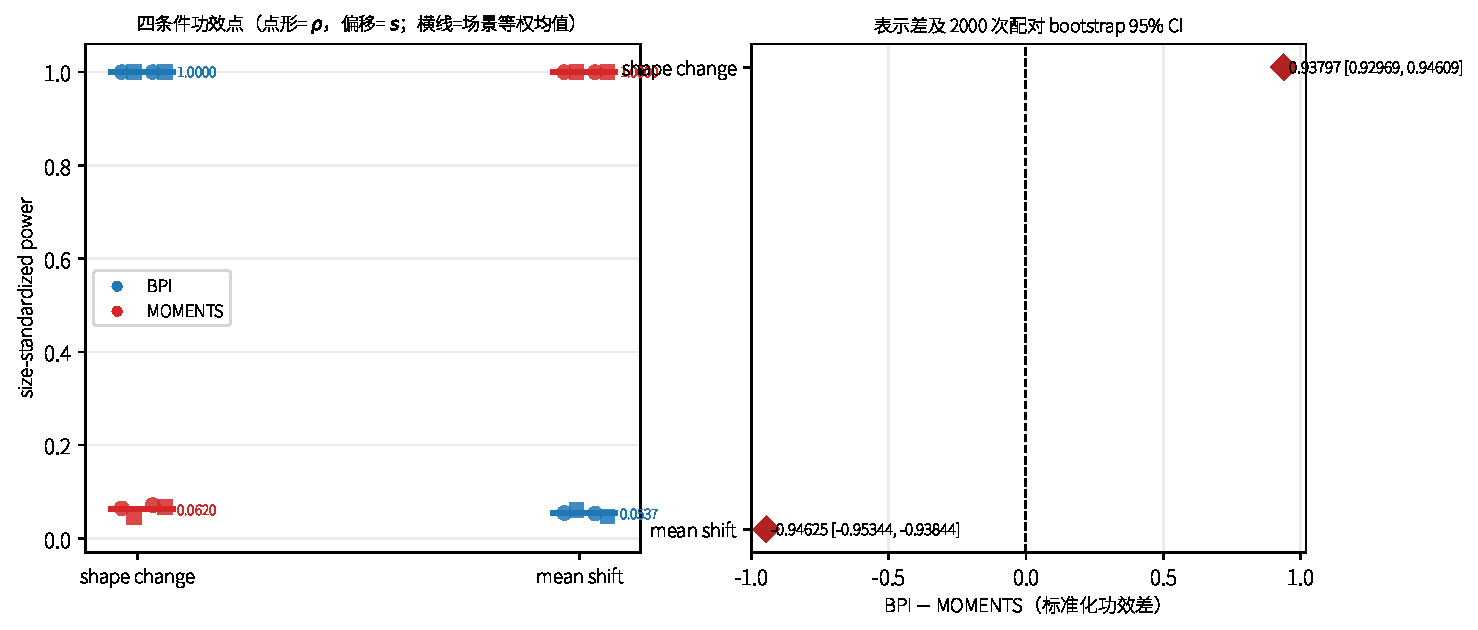
\includegraphics[width=0.95\textwidth]{../artifacts/figures/Figure5_H1_power_and_difference.pdf}
\caption{左：形状变化与均值平移下 BPI 与 MOMENTS 的条件级尺寸标准化功效。小点为四个预设条件之一（点形编码 $\rho$：圆圈 $\rho=0$，方块 $\rho=0.8$；水平偏移编码 $s$）；横线为场景等权平均功效。两个场景之间不使用连线，以避免暗示连续变化趋势。右：两个场景下 BPI 减去 MOMENTS 的功效差及 2000 次配对百分位自助 95\% 区间，零线表示无差异。右图区间只对应表示差异，不用作单个表示功效均值的误差条。完整 16 行条件级结果见补充材料。}\label{fig:h1-power}
\end{figure}

两个场景中出现的样本功效 $1.00000$ 表示 1600 次有限 Monte Carlo 重复在全部四个条件上的汇总结果，未构成总体功效恒等于 1 的概率保证。式\eqref{eq:shape-power-diff}与式\eqref{eq:mean-power-diff}共同支持表示选择性的结论：拓扑表示和矩表示保留了不同类型的变化信息，任何单一表示的检出能力均应结合备择结构加以评价。

\subsection{名义功效与尺寸标准化功效}\label{sec:h1-std}

直接以 $p\le0.05$ 计算的名义功效同时受到观测统计量和校准参考分布的影响。当对应零假设配置未达到点态实用校准时，名义功效可能因反保守性而被抬高，也可能因保守性而被压低。尺寸标准化功效改用匹配零假设统计量的经验临界值，使 BPI 与 MOMENTS 在各自零假设尺度上接受比较。该指标仍是条件化的有限样本量，不能消除表示维数、窗口参数和备择强度等设计因素的影响。

\subsection{定位误差与联合成功率}\label{sec:h1-localization}

位置估计由观测扫描曲线确定，按式\eqref{eq:location-map}映射回原始时间轴。由于变化在 $t=\lfloor T/2\rfloor$ 与 $t=\lfloor T/2\rfloor+1$ 之间发生，真实连续边界为
\begin{equation}\label{eq:true-location}
 \tau_{\mathrm{true}}=\left\lfloor\frac T2\right\rfloor+\frac12.
\end{equation}
本文报告无条件绝对误差
\[
 E_r=|\widehat\tau_r-\tau_{\mathrm{true}}|,
\]
原始尺度平均绝对误差 $R_1^{-1}\sum_rE_r$，以及归一化平均绝对误差
\begin{equation}\label{eq:normalized-mae}
 \operatorname{nMAE}
 =\frac1{R_1}\sum_{r=1}^{R_1}\frac{E_r}{T}.
\end{equation}
位置误差由观测统计量决定，因此对同一“条件--表示”组合，M0 与 M1 共享相同的 $\widehat\tau_r$。校准方法只通过拒绝事件影响联合成功率。对方法 $m\in\{\mathrm{M0},\mathrm{M1}\}$，定义
\begin{equation}\label{eq:joint-success}
 \widehat J_m
 =\frac1{R_1}\sum_{r=1}^{R_1}
 \mathbf1\left\{p_{r,m}\le0.05,\;
 |\widehat\tau_r-\tau_{\mathrm{true}}|\le\frac W2\right\}.
\end{equation}
漏检重复保留在式\eqref{eq:joint-success}的分母中，因此该量同时评价检出与定位。

表~\ref{tab:h1-power}以同一场景内四个预设条件的等权平均汇总功效、归一化定位误差和联合成功率。不同步长对应的 $T$ 不同，故正文采用式\eqref{eq:normalized-mae}保证条件间尺度可比；逐条件原始 MAE、匹配零假设临界值和对应 I 类错误率见补充材料。定位汇总由既有观测扫描结果重新计算，未改变或重跑 Monte Carlo 试次。

\input{../artifacts/tables/Table5_h1_power.tex}


% 本稿未纳入自然数据案例；外部验证边界在讨论部分明确说明。

\section{讨论}\label{sec:discussion}

\subsection{重叠窗口引起的随机化单位错配}\label{sec:disc-validity}

本文的理论和模拟共同表明，重叠窗口带来的推断问题超出了“相关样本使有效样本量下降”的标量解释范围。窗口重用首先改变派生特征的联合分布：即使原始观测独立同分布，相邻特征仍可能共享大量底层随机变量，并形成随窗口距离变化的协方差。全局随机置换操作保留经验边际分布，却打散原始顺序中的滞后协方差，因此科学零假设下的“无变化”无法自动提供窗口层面的排列不变性。命题~\ref{prop:counterexample}给出了这一层级错配的有限样本反例，式\eqref{eq:permutation-fpc}则说明排列参考的条件变异只由经验边际量决定。该机制与依赖时间序列中置换检验需要附加有效性条件的既有理论一致\cite{RomanoTirlea2022}。

有效样本量仍可作为特定线性统计量的直观概括。例如，$W=64$、$s=16$、$M=192$ 时，窗口均值的方差比约为 $3.974$。然而，窗口均值的方差比可以解释特定线性统计量的变异变化，但不能直接决定一般高维最大扫描的参考分布及其拒绝率。本文因此对完整检验逐条件开展模拟评价。

\subsection{双预算视角与条件化校准图谱}\label{sec:disc-surface}

固定窗口数和固定观测长度回答不同的条件问题。前者保持扫描序列长度 $M$ 不变，步长变化同时改变原始观测长度；后者保持 $T$ 不变，步长变化同时改变窗口数。两种制度均无法单独隔离所有设计因素，但它们提供了互补的预算视角。P1 与 P2 在两个预设数据生成过程的等权平均下均超过预设实质阈值，说明严重失校准并非某一种预算制度的偶然产物。相应结论仍应限定于本文的 $W$、步长网格、数据生成过程和表示实现。

校准图谱的概念还强调，汇总平均不能替代逐格有效性判断。朴素置换下，BPI 与 MOMENTS 的拒绝率范围分别为 $0.0472$--$0.9756$ 和 $0.0432$--$0.9996$。依赖乘子校准下，相应范围分别为 $0.0056$--$0.1180$ 和 $0.0020$--$0.1412$。将条件间的保守性与反保守性合并，可能得到接近 $0.05$ 的总体均值，同时掩盖局部严重失真。因此，本文将逐格拒绝率、Wilson 区间和预设实用等价带作为主要证据。该分类依赖 Monte Carlo 样本量和等价带宽度，属于操作性有限样本判据。

\subsection{依赖乘子校准的改善与局限}\label{sec:disc-dmb}

M1 在多数重叠配置中大幅降低了 M0 的极端反保守性，说明相关乘子在参考过程中引入了预设相关结构。不过，M1 仍同时产生实质保守和实质反保守配置。一般 dependent wild bootstrap 或依赖乘子理论主要针对特定均值、光滑函数或经验过程\cite{Shao2010,BucherKojadinovic2016}：Shao 的 dependent wild bootstrap 面向平稳序列的部分和近似，B{\"u}cher 与 Kojadinovic 的依赖乘子则针对强混合经验 copula 过程，二者均在各自函数类内给出渐近有效性。这些理论为窗口特征序列提供了渐近分析的起点，但均未提供本文完整 BPI 最大扫描在当前样本规模和固定带宽规则下的有限样本校准保证；其适用性仍需针对本文的局部映射、扫描泛函与带宽规则逐项验证。

当前带宽规则也有助于解释非重叠端的保守性。即使 $s=W$，式\eqref{eq:dmb-bandwidth}中的 $\lceil M^{1/3}\rceil$ 仍使 $b>1$；以 P3 的固定 $M=192$ 配置为例，$b=6$，相关乘子不会退化为独立乘子。P3 检出的保守偏差与这一结构相容，但本文没有进一步分解带宽、桥接和高维特征谱各自的贡献。后续研究可针对窗口依赖尺度推导步长适配的乘子协方差，或在原始时间轴上实施块重采样并重新构造全部窗口特征。此类扩展需要新的理论和独立确认实验。

\subsection{表示敏感性与校准有效性}\label{sec:disc-representation}

形状变化和均值平移中的功效反转说明，表示选择决定了观测统计量能够保留何种信号。BPI 在圆形到 8 字形曲线的变化中具有很高的尺寸校正功效，MOMENTS 在均值平移中具有对应优势。尺寸校正临界值减少了零假设校准松紧对这一比较的直接影响，因此结果更接近表示层面的信号选择性。与此同时，该比较仍受窗口宽度、表示超参数、变化强度和有限样本设计约束。

表示敏感性与校准有效性应作为两个不同评价维度。信息不足的表示难以通过更准确的校准获得高功效；失真的参考分布也会使信息充分的表示产生错误的显著性判断。两者在有限样本下还可能通过维数、依赖谱和乘子带宽发生交互，本文没有假设其统计独立或严格正交。定位结果进一步显示，观测扫描曲线决定无条件位置误差，校准方法通过拒绝事件影响“检出且定位成功”的联合概率；这两个指标回答的统计问题需要保持区分。

\subsection{实践含义}\label{sec:disc-practice}

对采用重叠窗口的拓扑变化检测，本文给出三条操作建议：\begin{enumerate}\item 将窗口视为派生统计单位，而非因原始观测独立同分布就直接实施窗口级全局随机置换；校准单位应显式声明。\item 方法报告应明确窗口宽度、步长、原始长度、窗口数与校准单位，并在与实际管线匹配的零假设下逐条件评估 I 类错误率，而非依赖单一汇总平均。\item 固定观测预算与固定窗口数对应不同部署约束，其结论不宜互相替代；依赖感知重采样可作为更合理的参考起点，但其带宽与有限样本行为仍需针对具体表示与扫描统计量验证。\end{enumerate}

\subsection{研究局限}\label{sec:limitations}

本文的结论具有以下局限。
\begin{enumerate}
\item BPI 网格、核宽、尺度上界、同调通道和 MOMENTS 构造均保持固定；本文未系统遍历表示超参数，也未研究特征维数与校准行为之间的敏感性。
\item 零假设仅包含 N-AR 与 N-CIRCLE 两类合成过程，主要结论依赖两个过程的等权设计；更广的非高斯、长记忆、异方差和非平稳零模型尚待检验。
\item 备择仅包括一种形状变化和一种均值平移。形状构造匹配单时点边际均值与协方差，但没有匹配完整滞后联合分布或二阶过程。
\item M1 是冻结的依赖感知参考方法，本文没有为完整 BPI 最大扫描建立新的有限样本或渐近有效性定理，当前带宽规则也未针对每个步长进行最优选择。
\item 逐格校准分类为点态判断，依赖预设等价带和 Monte Carlo 精度，不提供整个设计域上的同时保证。
\item 本稿未纳入自然数据或独立外部数据集，外部有效性主要由合成设计的覆盖范围限定。
\item 本文研究单一变点的最大扫描，尚未处理多变点递归、停止规则及相应的族错误率控制。
\end{enumerate}

\section{结论}\label{sec:conclusion}

本文评估了基于持续同调特征的变点检验在重叠滑动窗口下的有限样本校准。窗口均值反例说明，原始观测独立同分布不能自动保证派生窗口序列具有交换性。在所考察的设计网格内，朴素置换在两种表示的全部重叠配置中均表现为实质反保守；依赖乘子法普遍降低拒绝率，但在非重叠配置中表现为实质保守，未实现逐条件统一校准。原序列依赖对步长对比的影响随数据生成过程和表示变化。形状备择和整体平移负对照进一步表明，持续同调表示保留的结构信息及其不变性，需要与下游检验的误报控制分开解释。上述结论为当前固定实现提供有限样本参照，其范围由生成过程、窗口设计、表示参数和校准规则共同限定。


\section*{Data and Code Availability}
复现本文结果的代码、配置、种子清单、完整逐格数据与补充材料由仓库 \url{https://github.com/dw0911/owtda-calibration} 提供。本稿对应 git 标签 \texttt{v1.1.1-paper}；全部合成数据均由该版本代码与固定随机种子生成，不依赖外部数据归档，独立数据 DOI 尚在建立中，未作为已提供材料列出。补充材料 S5 给出代码入口与复现步骤。

\bibliographystyle{unsrt}
\bibliography{bibliography}
\end{document}
"`。
\newif\ifstrictfigures
\strictfiguresfalse
\IfFileExists{STRICT.tex}{\strictfigurestrue}{}

\let\OriginalIncludeGraphics\includegraphics
\RenewDocumentCommand{\includegraphics}{O{} m}{%
  \IfFileExists{#2}{%
    \OriginalIncludeGraphics[#1]{#2}%
  }{%
    \ifstrictfigures
      \PackageError{owtda-paper}{Strict build: missing figure `\detokenize{#2}'}%
        {The strict build (paper/STRICT.tex present) requires every figure to exist.}%
    \else
      \begin{minipage}[c][4.2cm][c]{0.82\linewidth}
        \centering\small 图件缺失：\texttt{\detokenize{#2}}
      \end{minipage}%
    \fi
  }%
}

\title{重叠窗口拓扑扫描的有限样本校准边界\\\large Finite-Sample Calibration Boundaries for Topological Change-Point Scans with Overlapping Windows}
\author{
  王平\textsuperscript{1}\quad
  黄盛南\textsuperscript{1}\quad
  张晓媛\textsuperscript{1,*}\\[2mm]
  \small $^1$河北金融学院统计与数据科学学院\\[1mm]
  \small 通讯作者：张晓媛，\texttt{zxy0407010229@163.com}
}
\date{2026年9月}

\begin{document}
\maketitle

\begin{abstract}
基于持续同调的时间序列变点检验可利用滑动窗口提取局部结构特征，但窗口共享观测引起的依赖可能使随机置换参考分布失真。本文考察固定持续图向量表示与最大扫描所构成检验的有限样本校准。首先，以高斯窗口均值构造反例，说明原始观测独立同分布仍不足以保证派生窗口序列的交换性。随后，在固定窗口数与固定原始观测长度两种设计下，对 28 个零假设配置比较无约束窗口级随机置换与依赖乘子自助法，并以均值--协方差特征作为非拓扑对照。在名义显著性水平 0.05 下，对每种表示，20 个重叠配置均表现为实质反保守，持续同调表示的经验拒绝率最高为 0.9756。依赖乘子法在全部匹配配置中降低拒绝率，但对每种表示，8 个非重叠配置均表现为实质保守；原序列依赖对步长对比的修饰方向随生成过程与表示变化。低阶矩匹配的圆形到 8 字形曲线备择下，两类表示的尺寸校正功效分别为 1.0000 和 0.0620；整体平移负对照则呈相反结果，与距离型持续同调的平移不变性一致。结果表明，当前实现的校准表现具有明确的条件依赖性，降低拒绝率不能等同于恢复名义校准，表示的信号敏感性与检验的误报控制应分别评价。

\noindent\textbf{关键词}：持续同调；变点检测；重叠滑动窗口；交换性；有限样本校准。

\end{abstract}

\section*{Abstract}
Change-point tests based on persistent homology use sliding windows to extract local structural features, but dependence induced by shared observations can distort random-permutation reference distributions. This study examines the finite-sample calibration of a test combining a fixed vector representation of persistence diagrams with a maximum scan statistic. A Gaussian window-mean counterexample first shows that independent and identically distributed raw observations do not ensure exchangeability of the derived window sequence. Naive unrestricted window-level permutation and a dependent multiplier bootstrap are then evaluated under fixed-window-count and fixed-observation-length designs across 28 null configurations, with mean--covariance features as a non-topological comparator. At the nominal level of 0.05, all 20 overlapping-window configurations are classified as materially anti-conservative for each representation; the empirical rejection rate for the persistent-homology representation reaches 0.9756. The multiplier procedure lowers rejection rates in every matched configuration, but all eight non-overlapping configurations are materially conservative for each representation. The effect of serial dependence on the stride contrast varies across generators and representations. Under a circle-to-figure-eight alternative with matched first and second marginal moments, size-adjusted powers are 1.0000 and 0.0620 for the persistent-homology and moment representations, respectively. A mean-shift negative control reverses this ordering, consistently with the translation invariance of distance-based persistent homology. These results demonstrate condition-dependent calibration for the studied implementation: lower rejection rates do not necessarily imply nominal calibration, and representation sensitivity and Type-I error control require separate evaluation.

\noindent\textbf{Keywords}: persistent homology; change-point detection; overlapping sliding windows; exchangeability; finite-sample calibration.


\section{引言}\label{sec:intro}

\subsection{研究背景与统计问题}\label{sec:intro-bg}

时间序列的结构变化既可能表现为均值、方差等低阶统计量的改变，也可能表现为局部轨迹几何、周期结构或状态空间形状的改变。滑动窗口和时延嵌入为后一类信号提供了局部化表示：每个时间片段被转换为点云，持续同调进一步从多尺度上提取连通分支和环等结构信息。相关理论奠定了滑动窗口持久性分析的基础\cite{PereaHarer2015}，持续图像等有限维表示则使持续图能够进入统计扫描和机器学习程序\cite{Adams2017}。近年来，拓扑摘要已被用于离线变点检测、在线监测及依赖序列中的结构异常识别\cite{IslambekovYuvarajGel2020,ZhengMakXieXie2023,ChazalLevrardRoyer2024,NieYue2026}。

为提高候选变点的扫描密度，实际分析常取步长 $s$ 小于窗口宽度 $W$。此时，相邻窗口共享原始观测，窗口特征序列由此形成局部依赖。设第 $i$ 个窗口经固定映射得到特征 $Y_i$。对全部窗口顺序实施置换时，有限样本精确性通常依赖联合分布对排列群保持不变，即
\begin{equation}\label{eq:intro-exchangeability}
 (Y_1,\ldots,Y_M)\overset{d}{=}(Y_{\pi(1)},\ldots,Y_{\pi(M)}),
 \qquad \forall\,\pi\in\mathfrak S_M.
\end{equation}
独立同分布是满足该条件的一种充分情形，排列操作直接要求的条件则是窗口特征层面的联合交换性。窗口共享观测可诱发局部依赖，但特定映射是否具有交换性取决于其联合分布；平稳性、边际同分布以及原始序列的独立同分布性质，在窗口重叠时均不足以一般性地推出式\eqref{eq:intro-exchangeability}。由此形成本文关注的统计错配：科学零假设定义在原始过程的“无变化”层面，置换校准所需的对称性定义在派生窗口特征的联合分布层面。依赖时间序列中的置换理论同样表明，未经修正的排列参考分布可能无法维持名义检验水平\cite{RomanoTirlea2022}；随机排列检验的有限样本有效性还需相应的群不变性条件\cite{HemerikGoeman2018}。

本文考察一种基于持续同调特征的变点检验：每个局部时间窗口映射为点云，点云经持续同调及固定向量化形成特征序列，再通过标准化部分和的最大值检测前后特征均值差异。持续同调决定检验保留的结构信息，重采样程序决定统计量的参考分布。本文重点评价窗口重叠对后者有限样本校准的影响，并以均值--协方差特征作为非拓扑对照。

\subsection{相关工作与研究缺口}\label{sec:intro-lit}

与本文相关的研究可概括为三条脉络。第一类工作研究滑动窗口嵌入、持续同调及持续图向量化，为局部时间片段的拓扑表示提供方法基础\cite{PereaHarer2015,Adams2017}，其关注点主要在于表示的稳定性与可解释性，而未系统考察重叠窗口下推断有效性的有限样本校准。第二类工作将拓扑摘要引入离线或在线变化检测，并显式处理时间依赖与误报控制：文献\cite{NieYue2026}已经分析重叠窗口下的依赖继承，并利用移动块自助法校准在线监测控制限；其它近邻工作则聚焦表示对结构变化的辨识能力及特定检测程序的性能\cite{IslambekovYuvarajGel2020,ZhengMakXieXie2023,ChazalLevrardRoyer2024}。本文沿用这一研究背景，固定表示、离线最大扫描和校准规则，比较两种观测预算下的零假设拒绝率与经验分类。第三类工作研究依赖数据下的置换、dependent wild bootstrap 与依赖乘子自助法，说明时间依赖会改变随机化参考分布，并为若干均值、光滑函数或经验过程问题建立渐近理论\cite{RomanoTirlea2022,Shao2010,BucherKojadinovic2016}。这些理论为窗口特征序列提供了渐近分析的起点，但其适用性仍需针对本文所用的局部映射、扫描泛函与带宽规则逐项验证。

这些结果尚未提供本文实现的具体有限样本保证：重叠局部窗口依次经过点云映射、持续同调向量化和最大扫描后，朴素置换会产生多大程度的有限样本尺寸失真；该失真如何随重叠程度、原序列依赖、观测预算和表示类型变化；依赖感知校准能够在哪些条件下减弱失真，又会在哪些条件下表现为保守或残留反保守。本文不以非线性变换本身主张该管线脱离既有理论框架，也不从渐近一致性推定当前样本规模下的名义尺寸控制，而以固定实现和预设设计网格上的有限样本校准偏差及其条件变化为考察重点。本文将条件组合 $\theta$ 下的有效检验水平记为 $\alpha_{\mathrm{eff}}(\theta)$，并将映射 $\theta\mapsto\alpha_{\mathrm{eff}}(\theta)$ 称为预设离散设计网格上的条件化有限样本校准图谱。本文不估计连续参数空间中的解析边界；“经验校准状态转换”仅指有序设计维度（主要为步长或重叠率）上相邻格点发生校准分类变化的位置。该图谱属于有限样本、点态和设计域内的刻画，不提供全参数空间的统一保证。

\subsection{研究目标与贡献}\label{sec:intro-contrib}

本文的主要贡献是对固定持续同调变点检验开展条件化有限样本校准评价：在两种预算设计和 28 个唯一零假设配置上，报告朴素置换与依赖乘子的拒绝率、区间及经验分类，并量化两种预算下重叠与非重叠条件之间的预设对比。机制分析通过一般局部映射的依赖继承和窗口均值反例说明交换性风险；备择分析通过低阶矩匹配的形状构造与整体平移负对照，解释固定表示的信号敏感性及不变性。理论推导、经验评价与构造对照分别承担机制、实际表现和解释功能。

全文其余部分安排如下：第~\ref{sec:method} 节定义重叠窗口特征、两类表示、最大扫描统计量及校准方法；第~\ref{sec:theory} 节分析有限依赖、交换性失效与方差机制；第~\ref{sec:protocol} 节说明评价对象和实验设计；第~\ref{sec:h0} 节报告零假设下的有限样本校准结果；第~\ref{sec:h1} 节分析备择下的检出与定位性能；第~\ref{sec:discussion} 节讨论方法含义、适用范围与局限；第~\ref{sec:conclusion} 节总结全文。

\section{基于持续同调特征的变点检验}\label{sec:method}

图~\ref{fig:flow}给出整体流程与统计冲突的来源：窗口是随机化单位，但重叠使原始观测被多个随机化单位共享。后续小节依次定义窗口构造、两种表示、最大扫描统计量与两种校准方法。

\begin{figure}[tbp]
\centering
\begin{subfigure}[t]{0.92\linewidth}
\centering
\caption{统计推断主流程}\label{fig:flow-a}
% 图 1(a)：重叠窗口拓扑扫描与校准的统计推断主流程（横向）。
% 依赖 main.tex 中定义的 flowblue/flowfill/m0fill/m1fill 配色与 tikz 库。
\begin{tikzpicture}[
  font=\footnotesize,
  box/.style={draw=flowblue, fill=flowfill, rounded corners=2pt,
              align=center, inner xsep=6pt, inner ysep=5pt, line width=0.6pt},
  arr/.style={-{Stealth[length=2.4mm]}, flowblue, line width=0.6pt},
]
\node[box] (raw) {原始序列\\ $X_1,\ldots,X_T$};
\node[box, right=4mm of raw] (win) {重叠滑动窗口\\ $I_1,\ldots,I_M$};
\node[box, right=4mm of win] (pc) {窗口点云\\ $P_i$};
\node[box, fill=m0fill, above right=3mm and 4mm of pc] (bpi) {持续同调 $\to$ 持续图\\ $\to$ BPI（800 维）};
\node[box, fill=m1fill, below right=3mm and 4mm of pc] (mom) {MOMENTS\\ （5/9 维）};
\coordinate (mid1) at ($(bpi.south east)!0.5!(mom.north east)$);
\node[box, right=4mm of mid1] (scan) {最大扫描\\ $T_M,\ \hat k$};

\node[box, fill=m0fill, below=15mm of scan, xshift=-19mm] (m0) {M0：全局随机置换重采样\\ $T_M^{*(1\ldots B)}$};
\node[box, fill=m1fill, below=15mm of scan, xshift=19mm] (m1) {M1：相关乘子重采样\\ （近似局部依赖）};

\coordinate (mid2) at ($(m0.south)!0.5!(m1.south)$);
\node[box, below=6mm of mid2] (ref) {参考分布 $\{T_M^*\}$\\ ＋ 观测 $T_M$};
\node[box, left=6mm of ref] (pv) {Monte Carlo\\ $p$ 值};
\node[box, left=6mm of pv] (dec) {拒绝 / 不拒绝\\ ＋ 位置估计 $\hat k$};

\draw[arr] (raw) -- (win);
\draw[arr] (win) -- (pc);
\draw[arr] (pc) -- (bpi);
\draw[arr] (pc) -- (mom);
\draw[arr] (bpi) -- (scan);
\draw[arr] (mom) -- (scan);
\draw[arr] (scan) -- (m0);
\draw[arr] (scan) -- (m1);
\draw[arr] (m0) -- (ref);
\draw[arr] (m1) -- (ref);
\draw[arr] (ref) -- (pv);
\draw[arr] (pv) -- (dec);
\end{tikzpicture}

\end{subfigure}

\vspace{1.2em}

\begin{subfigure}[t]{0.85\linewidth}
\centering
\caption{窗口重叠与共享观测机制}\label{fig:flow-b}
% 图 1(b)：窗口重叠与共享观测 + 全局随机置换破坏邻接。
\begin{tikzpicture}[
  font=\small,
  obs/.style={circle, draw=flowblue, fill=white, inner sep=1.2pt, line width=0.5pt},
  shared/.style={circle, draw=sharedred, fill=sharedred!25, inner sep=1.7pt, line width=0.6pt},
]
% 时间轴与观测
\foreach \i in {1,...,8} { \coordinate (X\i) at (\i, 0); }
\draw[flowblue, line width=0.5pt] (0.5,0) -- (8.5,0);
\foreach \i in {1,7,8} { \node[obs] at (X\i) {}; }
\foreach \i in {2,3,4,5,6} { \node[shared] at (X\i) {}; }
\foreach \i in {1,...,8} { \node[below=1.5mm, font=\footnotesize] at (X\i) {$X_{\i}$}; }

% 四个窗口（各覆盖 4 个连续观测，相邻窗口共享 3 个观测；与下方全局随机置换的 4 个窗口一致）
\draw[winblue, line width=1.3pt] (1,1.9) -- (4,1.9);
\draw[winblue, line width=0.8pt] (1,1.68) -- (1,2.12);
\draw[winblue, line width=0.8pt] (4,1.68) -- (4,2.12);
\node[right=1mm, font=\footnotesize] at (4,1.9) {窗口1};

\draw[winblue, line width=1.3pt] (2,1.35) -- (5,1.35);
\draw[winblue, line width=0.8pt] (2,1.13) -- (2,1.57);
\draw[winblue, line width=0.8pt] (5,1.13) -- (5,1.57);
\node[right=1mm, font=\footnotesize] at (5,1.35) {窗口2};

\draw[winblue, line width=1.3pt] (3,0.8) -- (6,0.8);
\draw[winblue, line width=0.8pt] (3,0.58) -- (3,1.02);
\draw[winblue, line width=0.8pt] (6,0.58) -- (6,1.02);
\node[right=1mm, font=\footnotesize] at (6,0.8) {窗口3};

\draw[winblue, line width=1.3pt] (4,0.25) -- (7,0.25);
\draw[winblue, line width=0.8pt] (4,0.03) -- (4,0.47);
\draw[winblue, line width=0.8pt] (7,0.03) -- (7,0.47);
\node[right=1mm, font=\footnotesize] at (7,0.25) {窗口4};

% 共享标注（置于窗口条上方）
\node[sharedred, font=\footnotesize] at (4.5,2.6) {共享观测（相邻窗口重叠 $W-s$ 个观测）};

% 全局随机置换示意（方块组居中于时间轴中心 x≈4.5，避免视觉偏左）
\foreach \i/\n in {1/1,2/2,3/3,4/4} {
  \node[draw=flowblue, fill=flowfill, minimum size=7mm, font=\footnotesize] at ({2.25+0.9*\i}, -2.3) {\n};
}
\node[left=2mm, font=\footnotesize] at (3.15,-2.3) {原始窗口序};
\foreach \i/\n in {1/3,2/1,3/4,4/2} {
  \node[draw=flowblue, fill=flowfill, minimum size=7mm, font=\footnotesize] at ({2.25+0.9*\i}, -3.8) {\n};
}
\node[left=2mm, font=\footnotesize] at (3.15,-3.8) {随机置换后};
\draw[-{Stealth[length=2mm]}, sharedred, line width=0.6pt] (3.6,-2.7) -- (3.6,-3.4);
\node[sharedred, right=2mm, font=\footnotesize] at (3.6,-3.05) {窗口级邻接被破坏};
\end{tikzpicture}

\end{subfigure}

\caption{基于持续同调特征的变点检验与校准流程。(a) 原始序列经重叠窗口映射为窗口点云，再分别经持续同调—向量化分支得到 BPI、经均值—协方差分支得到矩表示 MOMENTS，进入最大扫描得到检验统计量 $T_M$ 与位置估计 $\hat k$；随后 M0 无约束窗口级随机置换重采样、M1 相关乘子重采样分别构造参考分布，并通过 Monte Carlo $p$ 值形成拒绝决策。(b) 重叠机制：相邻窗口共享原始观测（红色），无约束窗口级随机置换重排窗口顺序时原有邻接被破坏，这是后文交换性失效机制的直观来源。}\label{fig:flow}
\end{figure}

\subsection{窗口构造与局部点云}\label{sec:windows}

给定观测序列 $X_1,\ldots,X_T$，取窗口宽度 $W$ 和步长 $s$，并令
\begin{equation}\label{eq:windows}
 a_i=(i-1)s+1,\qquad
 I_i=\{a_i,\ldots,a_i+W-1\},\qquad
 M=\left\lfloor\frac{T-W}{s}\right\rfloor+1.
\end{equation}
本文考虑 $1\le s\le W$，相邻窗口的名义重叠率为 $1-s/W$。对于二维观测，窗口点云直接定义为 $P_i=\{X_t:t\in I_i\}$。对于标量观测，在每个窗口内部构造三维时延点云
\begin{equation}\label{eq:delay-cloud}
 P_i=\bigl\{(X_t,X_{t+3},X_{t+6}):t=a_i,\ldots,a_i+W-7\bigr\},
\end{equation}
因而时延坐标不会跨越窗口边界。点云在计算持续同调前按固定规则进行精确去重；所有坐标尺度、网格、核宽和截断参数均预先设定，且不利用整条序列共同估计的自适应参数。该局部性条件将在第~\ref{sec:theory} 节用于界定窗口特征的依赖范围。

\subsection{固定网格持续强度表示}\label{sec:bpi}

对每个点云 $P_i$，在系数域 $\mathbb F_2$ 上按欧氏距离计算 Vietoris--Rips 持续同调，并保留 0 维和 1 维同调通道中有限且寿命为正的 birth--death 对。过滤采用边长阈值的直径约定：单形 $\sigma$ 的过滤值为其顶点间最大欧氏距离，即 $\operatorname{diam}(\sigma)$；尺度 $\varepsilon$ 下纳入所有满足 $\operatorname{diam}(\sigma)\le\varepsilon$ 的单形，即 $\operatorname{VR}_\varepsilon(P)=\{\sigma\subseteq P:\operatorname{diam}(\sigma)\le\varepsilon\}$。过滤不设数据驱动的截断上限，持续图坐标直接以欧氏距离尺度报告。由于有限欧氏点云的 Vietoris--Rips 过滤在过滤值达到点云直径时形成完全复形，所有 1 维同调类在此时均已消亡，仅最后一个 0 维连通分量的 death 为 $\infty$；实现中只丢弃该显式无限 death 分量，其余有限类全部保留。相关计算框架和有限维表示可分别参见\cite{Bauer2021,Adams2017}。

记 $K_i(\varepsilon)=\operatorname{VR}_\varepsilon(P_i)$。随过滤尺度 $\varepsilon$ 增大，复形形成嵌套序列 $K_i(\varepsilon)\subseteq K_i(\varepsilon')$（$\varepsilon\le\varepsilon'$）。零维同调记录连通分支，一维同调记录未被二维单形填充的独立循环；贝蒂数 $\beta_q(K_i(\varepsilon))=\dim H_q(K_i(\varepsilon);\mathbb F_2)$ 表示该尺度下相应同调空间的维数。持续同调进一步记录这些类随过滤尺度的出现与消失，由持续图中的 $(b,d)$ 概括，其中 $b$ 与 $d$ 分别为出生尺度与消亡尺度，$d-b$ 是过滤尺度上的寿命，而非真实时间轴上的持续时长。记第 $q\in\{0,1\}$ 个同调通道的持续图为
\[
 \mathcal D_i^{(q)}=\{(b_{ij}^{(q)},d_{ij}^{(q)})\}_j.
\]
给定场景固定的尺度上界 $c$，将每个有限持续图点转换为归一化 birth--lifetime 坐标。尺度上界 $c$ 仅用于该坐标缩放与截断，不用于提前终止过滤；过滤本身以 $+\infty$ 为阈值完整计算。
\begin{equation}\label{eq:bpi-normalization}
 u_{ij}^{(q)}=\min\left(\frac{b_{ij}^{(q)}}{c},1\right),\qquad
 v_{ij}^{(q)}=\min\left(\frac{d_{ij}^{(q)}-b_{ij}^{(q)}}{c},1\right).
\end{equation}
令 $\Delta=1/20$、$g_r=(r+1/2)\Delta$（$r=0,\ldots,19$）以及 $\sigma=0.05$。第 $q$ 个通道在网格中心 $(g_r,g_\ell)$ 上的持续强度坐标定义为
\begin{equation}\label{eq:bpi}
 Z_{i,r\ell}^{(q)}
 =\frac{\Delta}{2\pi\sigma^2}
 \sum_j v_{ij}^{(q)}
 \exp\left\{-\frac{(g_r-u_{ij}^{(q)})^2+(g_\ell-v_{ij}^{(q)})^2}{2\sigma^2}\right\}.
\end{equation}
每个同调通道产生 $20\times20=400$ 个坐标。按 0 维、1 维同调通道的顺序向量化并连接，再除以 $\sqrt 2$（该缩放使两个同调通道对总平方距离的贡献取等权平均），得到 800 维特征。此处涉及三类维数：同调维数 $q\in\{0,1\}$、点云所在空间维数 $d\in\{2,3\}$ 以及向量表示维数 $p=800$；$800$ 维特征不意味着本文研究了 $800$ 维拓扑。
\begin{equation}\label{eq:bpi-vector}
 Y_i^{\mathrm{BPI}}
 =\frac{1}{\sqrt2}
 \begin{bmatrix}
   \operatorname{vec}(Z_i^{(0)})\\
   \operatorname{vec}(Z_i^{(1)})
 \end{bmatrix}.
\end{equation}
空通道记为 400 维零向量。N-AR 时延点云取 $c=6$，圆形模型及其备择取 $c=2.5$。本文将每个持续图中以寿命加权的高斯核表面在固定网格中心进行评价，并将两个同调通道的结果拼接为向量，沿用实现标识 BPI。该表示与持续图像共享“持续图--加权核表面--有限维表示”的思路，但其离散化采用网格中心采样，区别于逐像素积分\cite{Adams2017}。BPI 仅标识本文的固定实现，不另行宣称一种标准 Betti 不变量，也不构成对随机持续图总体强度密度的估计\cite{WuKimRinaldo2023}。

\subsection{矩表示}\label{sec:moments}

为构造低阶统计摘要作为对照，设窗口点云为 $P_i=\{x_{ij}\}_{j=1}^{n_i}\subset\mathbb R^d$，并定义
\begin{equation}\label{eq:moments}
 \bar x_i=\frac1{n_i}\sum_{j=1}^{n_i}x_{ij},\qquad
 S_i=\frac1{n_i}\sum_{j=1}^{n_i}(x_{ij}-\bar x_i)(x_{ij}-\bar x_i)^\top.
\end{equation}
MOMENTS 特征依次连接均值、协方差对角元以及按固定字典序排列的 $\sqrt2(S_i)_{ab}$（$a<b$）：
\begin{equation}\label{eq:moments-vector}
 Y_i^{\mathrm{MOM}}
 =\bigl(\bar x_i^\top,(S_i)_{11},\ldots,(S_i)_{dd},
 \{\sqrt2(S_i)_{ab}:a<b\}\bigr)^\top.
\end{equation}
其维数为 $d(d+3)/2$，故二维和三维点云分别得到 5 维和 9 维特征。$\sqrt2$ 权重保证任意两个窗口 $i,j$ 满足
\begin{equation}\label{eq:moments-frob}
 \|Y_i^{\mathrm{MOM}}-Y_j^{\mathrm{MOM}}\|_2^2
 =\|\bar x_i-\bar x_j\|_2^2+\|S_i-S_j\|_F^2.
\end{equation}
该表示主要概括一、二阶矩；有限窗口和序列依赖仍可能使其响应某些形状变化，因此本文不预设其对所有拓扑变化均不敏感。

\subsection{最大扫描统计量与位置估计}\label{sec:scan}

本文采用的最大扫描统计量属于变点分析中标准化部分和型统计量的常见构造\cite{CsorgoHorvath1997}。对任一窗口特征序列 $Y_1,\ldots,Y_M\in\mathbb R^p$，令
\begin{equation}\label{eq:bridge}
 U_M(k)=\frac1{\sqrt M}
 \left(\sum_{i=1}^kY_i-\frac{k}{M}\sum_{i=1}^M Y_i\right),
 \qquad t_k=\frac{k}{M},
\end{equation}
并定义标准化扫描曲线与最大统计量
\begin{equation}\label{eq:scan}
 Q_M(k)=\frac{\|U_M(k)\|_2^2}{t_k(1-t_k)},\qquad
 T_M=\max_{k\in\mathcal K_M}Q_M(k),
\end{equation}
其中
\[
 \mathcal K_M=\{\lceil0.15M\rceil,\ldots,M-\lceil0.15M\rceil\},
\]
比例 $0.15$ 为确认性分析前固定的边界保护比例，用于避免左右片段过短。
等价地，若 $\bar Y_{1:k}$ 和 $\bar Y_{k+1:M}$ 分别表示左右两段样本均值，则
\begin{equation}\label{eq:scan-equivalent}
 Q_M(k)=\frac{k(M-k)}{M}
 \|\bar Y_{1:k}-\bar Y_{k+1:M}\|_2^2.
\end{equation}
因此，该扫描统计量直接响应左右两段窗口特征的均值之差，检验对象是特征均值层面的变化；它不构成对任意原始分布或任意拓扑变化都具有一致检出能力的通用检验。

对 BPI 表示，令 $V_i^{(q)}=\operatorname{vec}(Z_i^{(q)})$ 为第 $q$ 个同调通道的未缩放向量，并分别对每个通道使用相同的桥接与标准化，得到 $Q_M^{(q)}(k)$。由 $Y_i^{\mathrm{BPI}}=\frac1{\sqrt2}[V_i^{(0)};V_i^{(1)}]$ 及平方欧氏范数的线性性，对每个候选位置 $k$ 有
\[
 Q_M^{\mathrm{BPI}}(k)=\frac12 Q_M^{(0)}(k)+\frac12 Q_M^{(1)}(k).
\]
因此总扫描同时受连通分支持续信息与循环持续信息影响。由于最大值的位置通常不同，$\max_k\tfrac12\bigl(Q_M^{(0)}(k)+Q_M^{(1)}(k)\bigr)$ 一般不等于两个通道最大值的平均 $\tfrac12\max_k Q_M^{(0)}(k)+\tfrac12\max_k Q_M^{(1)}(k)$。本文实验将两个同调通道合并报告，未单独分离零维与一维同调的贡献。

为使浮点并列情形具有确定性，令 $\epsilon_{64}=2^{-52}$，将满足
\[
 Q_M(k)\ge T_M-64\epsilon_{64}\max(1,|T_M|)
\]
的连续候选段定义为合格平台。位置估计选取最长平台；长度并列时取最左平台，再以该平台的下中位数作为 $\widehat k$。由于 $k$ 表示第 $k$ 与第 $k+1$ 个窗口之间的分割，映射到原始时间轴后的连续边界估计为
\begin{equation}\label{eq:location-map}
 \widehat\tau=\left(\widehat k-\frac12\right)s+\frac{W+1}{2}.
\end{equation}
该映射将第 $\widehat k$ 与第 $\widehat k+1$ 个窗口之间的分割点对应到二者中心之间的中点。若特征序列精确恒定，则规定 $T_M=0$。所有校准方法均使用相同的观测统计量、候选集合和位置规则。

\subsection{校准方法}\label{sec:calibration}

朴素置换方法记为 M0。M0 从排列群 $\mathfrak S_M$ 上的均匀分布中独立抽取随机排列；下文称为全局随机置换，以区别于块置换或局部置换。条件于观测到的窗口特征，M0 对每个随机排列序列重新计算式\eqref{eq:scan}。该方法保留经验边际分布，却不保留原始窗口顺序中的局部依赖。

依赖乘子自助法记为 M1。令 $\bar Y=M^{-1}\sum_{i=1}^M Y_i$、$Z_i=Y_i-\bar Y$，并取
\begin{equation}\label{eq:dmb-bandwidth}
 b=\max\left\{\left\lfloor\frac Ws\right\rfloor+1,
                 \left\lceil M^{1/3}\right\rceil\right\}.
\end{equation}
乘子新息 $\varepsilon_1,\ldots,\varepsilon_{M+b-1}$ 为独立标准正态，由与观测样本分离的随机流生成，因而与观测样本相互独立；不同内层重复使用各自的随机流独立生成。定义
\begin{equation}\label{eq:dmb-multiplier}
 \xi_i=b^{-1/2}\sum_{j=0}^{b-1}\varepsilon_{i+j},
 \qquad i=1,\ldots,M.
\end{equation}
由此
\begin{equation}\label{eq:dmb-cov}
 \operatorname{Cov}(\xi_i,\xi_{i+h})
 =\left(1-\frac{|h|}{b}\right)_+.
\end{equation}
M1 不作循环回绕，并对乘子加权序列 $\{\xi_iZ_i\}_{i=1}^M$ 应用与观测样本相同的桥接扫描。该构造属于依赖感知的参考近似；dependent wild bootstrap 和依赖乘子过程的一般理论可参见\cite{Shao2010,BucherKojadinovic2016}，其结论不直接构成本文完整 BPI 最大扫描的有限样本有效性定理。

两种方法均使用 $B=999$ 次重采样。若
\[
 K=\sum_{r=1}^{B}\mathbf 1\{T_{M,r}^*\ge T_M\},
\]
则 Monte Carlo $p$ 值定义为
\begin{equation}\label{eq:mc-pvalue}
 p=\frac{K+1}{B+1}=\frac{K+1}{1000}.
\end{equation}
本文以 $p\le0.05$ 拒绝零假设，等价于 $K\le49$。加一形式避免有限重采样下报告零 $p$ 值\cite{PhipsonSmyth2010}，但不恢复重叠窗口的交换性，也不替代对 M1 参考近似有效性的评估；随机排列检验的有限样本有效性仍需相应的群不变性条件\cite{HemerikGoeman2018}。

\section{重叠窗口的交换性与方差机制}\label{sec:theory}

本节利用可解析的窗口均值构造说明重叠如何改变派生统计量的联合分布。对随机向量 $(Y_1,\ldots,Y_M)$，若对任意排列 $\pi\in\mathfrak S_M$ 都有
\[
 (Y_1,\ldots,Y_M)\overset d=(Y_{\pi(1)},\ldots,Y_{\pi(M)}),
\]
则称其具有交换性。以下结果依次讨论局部映射的依赖范围、交换性反例、有限样本方差以及排列参考与原始顺序之间的协方差差异。相关结论用于解释失校准机制，不直接给出一般拓扑最大扫描的误报率公式。

\subsection{窗口局部映射的依赖范围}\label{sec:t1}

固定局部窗口映射的依赖继承是后续机制分析的基础，相关结果已见文献\cite{NieYue2026}（附录命题 6）。为明确本文的窗口与映射条件，下面给出原始观测独立同分布情形的自包含证明。

\begin{proposition}[局部映射的有限依赖范围]\label{prop:dependency}
设原始观测 $\{X_t\}$ 独立同分布，且
\[
 Y_i=\Psi\bigl((X_t)_{t\in I_i}\bigr),
\]
其中 $\Psi$ 为固定可测映射，并且不使用由整条序列共同估计的参数。则 $\{Y_i\}$ 至多为
\[
 m=\left\lceil\frac Ws\right\rceil-1
\]
阶依赖序列。
\end{proposition}

\begin{proof}
取任意两个窗口指标集合 $A,B\subset\{1,\ldots,M\}$，并假设 $\min_{i\in A,j\in B}|i-j|>m$。对任意 $i\in A$ 与 $j\in B$，不妨设 $i<j$，则
$$(j-i)s\ge\left\lceil W/s\right\rceil s\ge W,$$
从而 $I_i\cap I_j=\varnothing$。因此，$\{X_t:t\in\cup_{i\in A}I_i\}$ 与 $\{X_t:t\in\cup_{j\in B}I_j\}$ 生成的两个 $\sigma$-代数相互独立，其固定可测函数 $\{Y_i:i\in A\}$ 与 $\{Y_j:j\in B\}$ 也相互独立。由 $m$-依赖的定义即得结论。
\end{proof}

命题~\ref{prop:dependency}给出依赖范围的上界。窗口发生重叠时，具体协方差是否为零仍取决于原始分布和映射 $\Psi$；局部依赖也不自动等同于不可交换性，后者需要考察完整联合分布。

\subsection{交换性失效的精确反例}\label{sec:t2}

\begin{proposition}[高斯窗口均值的非交换性]\label{prop:counterexample}
设 $X_t\overset{\mathrm{iid}}{\sim}N(0,\sigma^2)$，其中 $\sigma^2>0$；设 $1\le s<W$ 且窗口数 $M\ge3$。记 $(x)_+=\max(x,0)$。令
\[
 Z_i=\frac1W\sum_{t\in I_i}X_t.
\]
则对 $h=0,\ldots,M-1$ 及 $i=1,\ldots,M-h$，
\begin{equation}\label{eq:window-cov}
 \Gamma_h=\operatorname{Cov}(Z_i,Z_{i+h})
 =\frac{\sigma^2}{W^2}(W-hs)_+,
\end{equation}
且随机向量 $(Z_1,\ldots,Z_M)$ 不具交换性。
\end{proposition}

\begin{proof}
由于原始观测相互独立，只有两个窗口共享的观测指标对协方差有贡献。交集 $I_i\cap I_{i+h}$ 含有 $(W-hs)_+$ 个指标，故得到式\eqref{eq:window-cov}。又因 $1\le s<W$，有
\[
 \Gamma_1=\frac{\sigma^2}{W^2}(W-s)
 >\frac{\sigma^2}{W^2}(W-2s)_+=\Gamma_2.
\]
考虑交换第 2、3 个坐标的排列。交换前，第一坐标与第二、第三坐标的协方差分别为 $\Gamma_1$ 和 $\Gamma_2$；交换后两者互换。协方差矩阵由此发生改变。高斯向量的分布由均值和协方差矩阵唯一确定，因此交换后的联合分布与原分布不同。
\end{proof}

\begin{remark}
该反例说明，原始观测的独立同分布性质不足以保证重叠窗口统计量具有交换性。结论并未覆盖所有固定局部映射，例如常数映射始终产生可交换序列。条件 $M\ge3$ 也具有实质作用：当 $M=2$ 时，两个等方差的联合高斯窗口均值具有对称协方差矩阵，交换两个坐标不会改变其分布。
\end{remark}

\subsection{窗口均值的有限样本方差比}\label{sec:t3}

\begin{proposition}[窗口均值的精确方差比]\label{prop:variance}
在命题~\ref{prop:counterexample}的构造下，令
\[
 \bar Z_M=\frac1M\sum_{i=1}^M Z_i,
 \qquad \Gamma_0=\frac{\sigma^2}{W}.
\]
则
\begin{align}
 \operatorname{Var}(\bar Z_M)
 &=\frac{\Gamma_0}{M}A_{\mathrm{mean},M},\label{eq:mean-var}\\
 A_{\mathrm{mean},M}
 &=1+2\sum_{h=1}^{M-1}
 \left(1-\frac hM\right)
 \left(1-\frac{hs}{W}\right)_+.
 \label{eq:finite-vif-general}
\end{align}
若 $W=qs$、$q$ 为正整数且 $M\ge q$，则
\begin{equation}\label{eq:finite-vif}
 A_{\mathrm{mean},M}=q-\frac{q^2-1}{3M}.
\end{equation}
\end{proposition}

\begin{proof}
按滞后展开协方差和，
\[
 M^2\operatorname{Var}(\bar Z_M)
 =M\Gamma_0+2\sum_{h=1}^{M-1}(M-h)\Gamma_h.
\]
将式\eqref{eq:window-cov}代入并除以 $M^2$，即可得到式\eqref{eq:mean-var}--\eqref{eq:finite-vif-general}。当 $W=qs$ 且 $M\ge q$ 时，非零求和项仅为 $h=1,\ldots,q-1$。利用
\[
 \sum_{h=1}^{q-1}\left(1-\frac hq\right)=\frac{q-1}{2},
 \qquad
 \sum_{h=1}^{q-1}h\left(1-\frac hq\right)=\frac{q^2-1}{6},
\]
整理后得到式\eqref{eq:finite-vif}。
\end{proof}

在本文的一个主要几何配置 $W=64$、$s=16$、$M=192$ 下，$q=4$，故
\[
 A_{\mathrm{mean},M}=4-\frac{15}{576}\approx3.974.
\]
该数值描述标量窗口均值相对于独立窗口基准的方差比。BPI 最大扫描还受到高维方向、特征谱和极值操作影响，因此不能将 $3.974$ 解释为其 I 类错误率的膨胀倍数。

\subsection{长期协方差与排列参考的错配}\label{sec:t4}

当 $W=qs$ 时，标量窗口均值为 $(q-1)$-依赖序列，其长期方差为
\begin{equation}\label{eq:long-run-var}
 \Omega
 =\sum_{h=-\infty}^{\infty}\Gamma_h
 =\Gamma_0+2\sum_{h=1}^{q-1}\Gamma_h
 =q\Gamma_0.
\end{equation}
只要 $q>1$，就有 $\Omega>\Gamma_0$。原始顺序下的部分和变异包含滞后协方差，随机排列参考则主要由窗口值的经验边际变异决定。

这一差别可由有限总体恒等式进一步说明。给定 $z_1,\ldots,z_M$，令
\[
 \bar z=\frac1M\sum_{i=1}^M z_i,
 \qquad
 s_M^2=\frac1M\sum_{i=1}^M(z_i-\bar z)^2,
\]
并令 $\pi$ 为 $\{1,\ldots,M\}$ 上的均匀随机排列。对 $1\le k<M$，
\begin{equation}\label{eq:permutation-fpc}
 \operatorname{Var}_{\pi}\left[
 \frac1{\sqrt M}\sum_{i=1}^k(z_{\pi(i)}-\bar z)
 \,\middle|\,z_1,\ldots,z_M\right]
 =\frac{k(M-k)}{M(M-1)}s_M^2.
\end{equation}
式\eqref{eq:permutation-fpc}源于不放回抽样中不同抽取位置的条件协方差 $-s_M^2/(M-1)$。因此，排列桥接过程的条件变异由经验边际量 $s_M^2$ 决定，而原始窗口顺序还携带式\eqref{eq:long-run-var}所概括的滞后依赖。该机制与依赖时间序列中置换有效性需要附加条件的结论一致\cite{RomanoTirlea2022}。

协方差结构的差异为失校准提供了机制解释。对于一般多维非线性特征，协方差矩阵不相等本身仍不足以推出最大扫描统计量的极限分布必然不同；同样，重叠率增加也不保证每一种表示或校准器的 I 类错误率单调变化。

上述结果证明，窗口重叠能够破坏窗口级随机化所需的联合对称条件，并揭示全局随机置换遗漏原顺序滞后协方差的机制；但这些解析结果没有给出 BPI 最大扫描的有限样本误报率闭式表达。因此，第~\ref{sec:h0} 节通过预设设计网格上的 Monte Carlo 实验评估完整非线性管线的实际有限样本校准。

\section{实验设计与评价规约}\label{sec:protocol}

\subsection{评价对象与操作性定义}\label{sec:estimands}\label{sec:rq}

令
\[
 \theta=(g,\rho,s,r,\varphi,\mathcal C)
\]
表示一个完整的零假设条件，其中 $g$ 为数据生成过程，$\rho$ 为原序列依赖参数，$s$ 为窗口步长，$r\in\{\mathrm{fixed}\text{-}M,\mathrm{fixed}\text{-}T\}$ 为预算制度，$\varphi\in\{\mathrm{BPI},\mathrm{MOMENTS}\}$ 为表示，$\mathcal C\in\{\mathrm{M0},\mathrm{M1}\}$ 为校准方法。名义显著性水平固定为 $\alpha=0.05$。本文的有效检验水平指配置条件下的零假设拒绝概率，并以 Monte Carlo 经验 I 类错误率估计；它不构成对整个零假设族取上确界的复合检验 size。该配置条件下的拒绝概率定义为
\begin{equation}\label{eq:effective-size}
 \alpha_{\mathrm{eff}}(\theta)
 =\Pr_{H_0,\theta}\{p_\theta\le0.05\}.
\end{equation}
映射 $\theta\mapsto\alpha_{\mathrm{eff}}(\theta)$ 构成本文的有限样本校准图谱（“图谱”仅指预设设计网格上的拒绝概率及经验分类，不指估计了连续响应面）。本文所称经验校准状态转换，是预设设计网格中有序设计维度（主要为步长或重叠率）上相邻格点发生校准分类变化的位置。

每个零假设配置均报告拒绝率及无连续性修正的 Wilson 区间\cite{Wilson1927}。预先冻结的实用等价带为
\[
 \mathcal E=[0.035,0.065].
\]
逐格分类规则如下：90\% Wilson 区间完整包含于 $\mathcal E$ 时，记为点态实用校准；95\% Wilson 区间上界低于 $0.035$ 时，记为实质保守；95\% Wilson 区间下界高于 $0.065$ 时，记为实质反保守；其余情形记为未定（未满足任一分类判据，不代表参数恰好位于真实边界）。该分类属于点态判断，不构成设计域上的同时概率保证。

备择实验考察两个相互关联的对象：其一，使用匹配零假设经验临界值计算的尺寸校正功效，用于比较表示所保留的信号信息；其二，基于观测扫描曲线得到的定位误差和“检出且定位成功”的联合概率。相应定义见第~\ref{sec:alternatives} 节和第~\ref{sec:h1-localization} 节。

\subsection{零假设数据生成过程}\label{sec:dgp}

首先生成平稳高斯 AR(1) 过程
\begin{equation}\label{eq:latent-ar}
 G_t=\rho G_{t-1}+\sqrt{1-\rho^2}\,\varepsilon_t,
 \qquad
 G_0\sim N(0,1),\quad
 \varepsilon_t\overset{\mathrm{iid}}{\sim}N(0,1),
\end{equation}
其中 $G_0$ 与全部新息相互独立，$\rho\in\{0,0.8\}$。实现中舍弃最初 1000 个值；由于初值取自平稳分布，该步骤作为统一的生成约定保留。

N-AR 直接取标量观测
\begin{equation}\label{eq:n-ar}
 X_t=G_t.
\end{equation}
N-CIRCLE 先以标准正态分布函数 $\Phi$ 作概率积分变换，再映射到单位圆：
\begin{equation}\label{eq:n-circle}
 U_t=\Phi(G_t),\qquad
 C(u)=(\cos 2\pi u,\sin 2\pi u),\qquad
 X_t=C(U_t)+0.08\eta_t,
\end{equation}
其中 $\eta_t\overset{\mathrm{iid}}{\sim}N_2(0,I_2)$，并与潜变量过程独立。对每个固定 $t$，$U_t$ 服从 $U(0,1)$；当 $\rho=0$ 时，两类原始过程均为独立同分布序列，当 $\rho=0.8$ 时则保留时间依赖。N-CIRCLE 的定义基于平稳高斯过程的边际变换，不涉及随机游走或增量过程。两个数据生成过程覆盖两类典型观测形态：N-AR 为标量序列，须经时延嵌入形成点云，对应一维时间序列场景；N-CIRCLE 为二维序列，窗口点云直接进入持续同调，对应多维观测场景。其潜在无噪声曲线具有圆形几何；加入观测噪声后，含噪观测分布的严格支撑为整个 $\mathbb R^2$，但有限点云在所考察过滤尺度上仍呈现明显的环状持续结构，便于考察拓扑表示对循环结构变化的敏感性。依赖水平取 $\rho\in\{0,0.8\}$，分别对应独立同分布与较强时间依赖两种端点情形，用于检验交换性失效对原序列依赖程度的敏感性。

\subsection{双预算制度}\label{sec:budget}

窗口宽度在确认性分析前固定为 $W=64$；本文不对该取值的最优性作主张。步长取
\[
 s\in\{8,16,32,64\},
\]
对应名义重叠率 $1-s/W$ 依次为 $87.5\%$、$75\%$、$50\%$ 与 $0$，覆盖从高重叠到无重叠的梯度，用于刻画重叠程度对校准的影响。
本文采用两种互补的预算制度：
\begin{itemize}
\item \textbf{固定窗口数（fixed-$M$）}：令 $M=192$，并由 $T=W+s(M-1)$ 确定原始序列长度；对应的 $T$ 依次为 $1592$、$3120$、$6176$ 和 $12288$。
\item \textbf{固定观测长度（fixed-$T$）}：令 $T=3120$，并由式\eqref{eq:windows}确定窗口数；对应的 $M$ 依次为 $383$、$192$、$96$ 和 $48$。
\end{itemize}
固定窗口数制度保持扫描器接收的特征数量不变，固定观测长度制度保持原始数据预算不变。两种制度在 $s=16$ 时共享相同的 $(T,M)=(3120,192)$ 几何配置；共享配置按同一逻辑实验单元计数。因此，$2$ 个数据生成过程、$2$ 个依赖水平和两种预算制度最终形成 28 个唯一零假设配置。

表~\ref{tab:design}给出两种预算制度下的完整窗口几何。该表同时说明：7 个唯一窗口几何的来源；两种制度在 $s=16$ 处的共享；$T$ 与 $M$ 如何随制度和步长变化；以及 M1 依赖乘子带宽为何随配置改变。

\begin{table}[ht]
\centering
\caption{双预算制度下的窗口几何设计。重叠率为 $1-s/W$；$b$ 为 M1 依赖乘子带宽，按 $b=\max\{\lfloor W/s\rfloor+1,\lceil M^{1/3}\rceil\}$ 确定。}\label{tab:design}
\begin{tabular}{cccccccc}
\toprule
$s$ & 重叠率 & \multicolumn{3}{c}{固定窗口数（fixed-$M$）} & \multicolumn{3}{c}{固定观测长度（fixed-$T$）}\\
\cmidrule(lr){3-5}\cmidrule(lr){6-8}
 & $1-s/W$ & $T$ & $M$ & $b$ & $T$ & $M$ & $b$\\
\midrule
8 & 87.5\% & 1592 & 192 & 9 & 3120 & 383 & 9 \\
16 & 75.0\% & 3120 & 192 & 6 & 3120 & 192 & 6 \\
32 & 50.0\% & 6176 & 192 & 6 & 3120 & 96 & 5 \\
64 & 0.0\% & 12288 & 192 & 6 & 3120 & 48 & 4 \\
\bottomrule
\end{tabular}

\begin{minipage}{0.94\textwidth}
\vspace{0.4em}
\footnotesize 注：$s=16$ 行在两种制度下给出相同的 $(T,M)=(3120,192)$，为共享配置；唯一配置计数中只计一次，但在两种预算视角下分别用于解释，因此该行会被两张热图有意重复展示。$s=64$ 时 $s=W$，窗口不重叠，重叠率为 0，对应 M1 保守性主对比 P3 的非重叠端。
\end{minipage}
\end{table}



图~\ref{fig:alternatives}展示两类备择构造的几何形态。

\begin{figure}[ht]
\centering
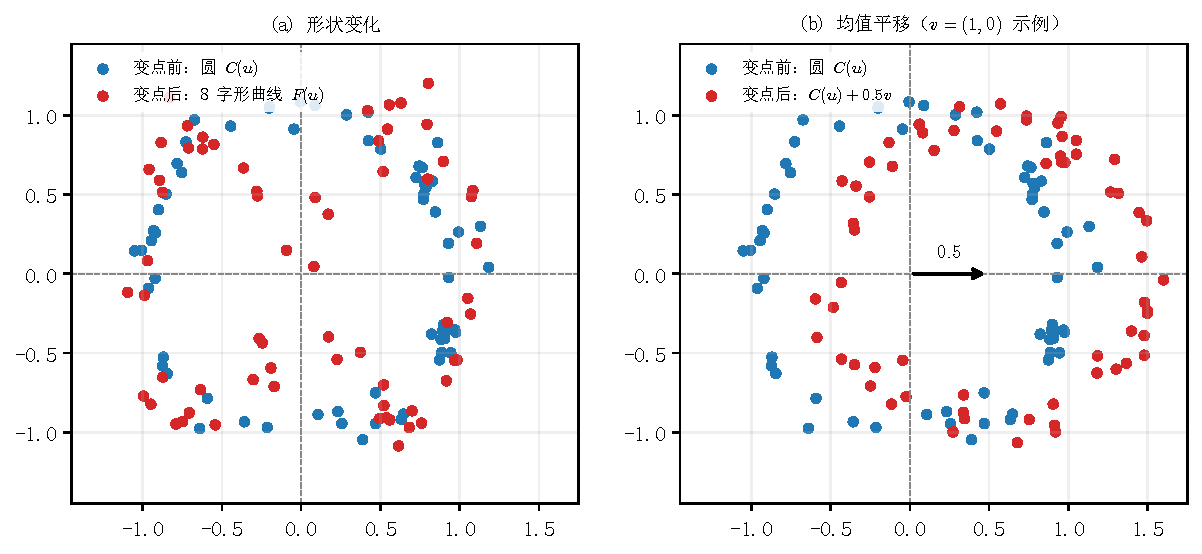
\includegraphics[width=0.95\textwidth]{../artifacts/figures/Figure2_alternative_geometry.pdf}
\caption{两类备择构造。(a) 形状变化：变点前为圆 $C(U_t)=(\cos2\pi U_t,\sin2\pi U_t)$，变点后改为 8 字形曲线 $F(U_t)=(\sin2\pi U_t,\sin4\pi U_t)$；(b) 均值平移：变点后整体平移 $+0.5v$，图中 $v=(1,0)$ 为示例方向，正式实验中 $v$ 跨重复随机、重复内固定。散点为含观测噪声 $0.08\eta_t$ 的 64 个点；圆与 8 字形曲线仅匹配单时点均值与协方差，完整滞后联合分布未被声明为相同。两个场景分别针对 BPI 与 MOMENTS 的结构敏感性。}\label{fig:alternatives}
\end{figure}

\subsection{Monte Carlo 设置}\label{sec:mc}

每格内部 $R_0=2500$（零假设）或 $R_1=1600$（备择）次主重复相互独立；不同格之间按主重复编号保留配对结构。每次方法校准均使用 $B=999$ 次内层重采样，并按式\eqref{eq:mc-pvalue}计算 $p$ 值。零假设部分包含
\[
 28\times2\text{（表示）}\times2\text{（方法）}\times2500
 =280{,}000
\]
条方法--表示评价记录；备择部分包含
\[
 2\text{（场景）}\times4\text{（条件）}\times2\text{（表示）}
 \times2\text{（方法）}\times1600
 =51{,}200
\]
条记录。外层 Monte Carlo 因而同时包含数据生成随机性与 $B=999$ 次内层校准的有限重采样随机性。

\subsection{预先设定的主对比}\label{sec:primary}

令 $\pi_{g,\rho,s,m}^{(r)}$ 表示在 BPI 表示、预算制度 $r$ 和校准方法 $m\in\{\mathrm{M0},\mathrm{M1}\}$ 下的零假设拒绝概率，且 $g\in\mathcal G=\{\mathrm{N\mbox{-}AR},\mathrm{N\mbox{-}CIRCLE}\}$。三个主对比均在确认性分析前冻结：
\begin{align}
\mathrm{P1}:\quad & D_{\mathrm{OV}}^{M}
 =\frac12\sum_{g\in\mathcal G}
 \left(\pi_{g,0,16,\mathrm{M0}}^{(M)}
      -\pi_{g,0,64,\mathrm{M0}}^{(M)}\right),
 \label{eq:p1}\\
\mathrm{P2}:\quad & D_{\mathrm{ST}}^{T}
 =\frac12\sum_{g\in\mathcal G}
 \left(\pi_{g,0,16,\mathrm{M0}}^{(T)}
      -\pi_{g,0,64,\mathrm{M0}}^{(T)}\right),
 \label{eq:p2}\\
\mathrm{P3}:\quad & D_{\mathrm{CONS}}
 =0.05-\frac12\sum_{g\in\mathcal G}
 \pi_{g,0,64,\mathrm{M1}}^{(M)}.
 \label{eq:p3}
\end{align}
P1 与 P2 检验单侧假设 $D\le0.10$ 对 $D>0.10$；P3 检验 $D_{\mathrm{CONS}}\le0.01$ 对 $D_{\mathrm{CONS}}>0.01$。阈值 $0.10$ 与 $0.01$ 均为查看确认性结果前规定的最小实质差异：$0.10$ 对应两个数据生成过程等权平均下至少 10 个百分点的 I 类错误率差异，$0.01$ 对应相对于名义水平 $0.05$ 至少 1 个百分点的保守偏差。MOMENTS 的同构对比仅作次级描述，不进入主要多重性族。

主对比使用 10,000 次按数据生成过程分层的整簇自助法。同一主重复编号下的全部相关条件、表示和方法随簇共同重采样，以保留配对结构。对一般效应量 $\widehat\theta$ 及单侧阈值 $\theta_0$，自助 $p$ 值定义为
\begin{equation}\label{eq:bootstrap-p}
 p_{\mathrm{boot}}
 =\frac{1+\sum_{b=1}^{10000}
 \mathbf1\{\widehat\theta_b^*-\widehat\theta
 \ge \widehat\theta-\theta_0\}}
 {10001}.
\end{equation}
因此，自助 $p$ 值不可能等于零。若 $q_\gamma$ 表示 10,000 个自助估计的最近秩（nearest-rank）$\gamma$ 分位数，则边际 95\% 基本型自助区间（basic bootstrap interval）\cite{DavisonHinkley1997}为
\begin{equation}\label{eq:basic-ci}
 \left[2\widehat\theta-q_{0.975},\,
       2\widehat\theta-q_{0.025}\right],
 \qquad
 q_\gamma=\widehat\theta^*_{(\lceil10000\gamma\rceil)}.
\end{equation}
三个单侧 $p$ 值采用 Holm step-down 校正\cite{Holm1979}，族水平为 $0.05$。本文将校正后 $p\le0.05$ 作为预先设定的操作性支持标准，同时用式\eqref{eq:basic-ci}报告效应量不确定性；该区间为边际区间，不解释为 Holm 同时置信区间。

\subsection{备择构造与尺寸校正功效}\label{sec:alternatives}

备择实验以 N-CIRCLE 为基础，并在完整序列上连续生成同一潜变量过程和观测噪声，不在变点处重置随机状态。令
\[
 \tau=\left\lfloor\frac T2\right\rfloor,
 \qquad
 F(u)=(\sin2\pi u,\sin4\pi u).
\]
形状变化场景定义为
\begin{equation}\label{eq:shape-alt}
 X_t=
 \begin{cases}
 C(U_t)+0.08\eta_t, & t\le\tau,\\
 F(U_t)+0.08\eta_t, & t>\tau.
 \end{cases}
\end{equation}
当 $U_t\sim U(0,1)$ 时，$C(U_t)$ 与 $F(U_t)$ 的单时点均值均为零，协方差均为 $I_2/2$；加入同分布噪声后，这两个单时点边际矩仍保持匹配。该构造不要求变点前后的完整滞后联合分布或二阶过程相同。

该备择旨在改变潜在几何中的独立循环结构，同时匹配单时点一、二阶矩：无噪声圆 $C([0,1])$ 同胚于 $S^1$，8 字形曲线 $F([0,1])$ 同胚于 $S^1\vee S^1$，二者在 $\mathbb F_2$ 系数下的一阶 Betti 数分别为 $1$ 和 $2$。但这一事实属于潜在连续曲线；有限含噪点云经 Vietoris--Rips 过滤后的持续图取决于抽样、噪声与尺度，不能被保证恰好分别产生一条与两条长寿命条带。本文实际检验的对象仍是有限点云持续图向量的均值变化。

均值平移场景定义为
\begin{equation}\label{eq:mean-alt}
 X_t=C(U_t)+0.08\eta_t+0.5v\mathbf1\{t>\tau\},
 \qquad
 v=(\cos2\pi V,\sin2\pi V),\quad V\sim U(0,1),
\end{equation}
其中方向变量 $V\sim U(0,1)$ 由独立随机流生成，与潜变量过程、观测噪声相互独立；每次 Monte Carlo 重复抽取一个方向 $v$，并在该重复内固定。每个备择场景均使用 $M=192$、$s\in\{16,64\}$ 和 $\rho\in\{0,0.8\}$，共四个条件。

尺寸校正功效使用与备择条件、表示和几何配置匹配的零假设观测统计量。将 $R_0=2500$ 个零假设统计量按升序记为
\[
 T_{M,(1)}^{H_0}\le\cdots\le T_{M,(R_0)}^{H_0},
\]
并令
\begin{equation}\label{eq:h0-critical}
 j_{0.95}=\left\lceil0.95(R_0+1)\right\rceil=2376,
 \qquad
 \widehat c_{0.95}^{H_0}=T_{M,(2376)}^{H_0}.
\end{equation}
对备择统计量 $T_{M,r}^{H_1}$，定义
\begin{equation}\label{eq:size-adjusted-power}
 \widehat\beta_{\mathrm{std}}
 =\frac1{R_1}\sum_{r=1}^{R_1}
 \mathbf1\{T_{M,r}^{H_1}>\widehat c_{0.95}^{H_0}\}.
\end{equation}
由于 M0 与 M1 共享同一观测统计量，式\eqref{eq:size-adjusted-power}在每个“条件--表示”组合上只计算一次，用于评价表示敏感性，不用于排列两种校准方法的优劣。

场景层面的表示差 $\Delta$ 通过两层整簇自助法估计。重采样单位为主复制（cluster）：零假设层按 N-CIRCLE 主复制整簇重采样以重算经验临界值，备择层按备择主复制整簇重采样以重算功效；共进行 2000 个联合 bootstrap 重复，每次分别独立重采样 H0 簇和 H1 簇，并产生一个场景差值。BPI 与 MOMENTS 使用同一重采样索引成对移动，四个 $(\rho,s)$ 条件在每个场景内先计算各自的 BPI 减 MOMENTS 功效差，再等权平均得到场景差。区间采用最近秩法（nearest-rank）定义的 2000 次百分位区间（$2.5\%$ 与 $97.5\%$ 分位数）。

\subsection{可复现性说明}\label{sec:repro}

实验协议、随机种子、配置和主要分析规则均在查看正式结果前确定。零假设与备择结果来自不可变的正式试次记录，正文数值由统一汇总文件生成。代码、环境文件、规范化结果和完整逐格输出由冻结的软件 release 提供，其地址见文末 Data and Code Availability。

\section{零假设下的有限样本校准结果}\label{sec:h0}

本节报告 28 个唯一零假设配置下，朴素置换（M0）与依赖乘子自助法（M1）的有限样本 I 类错误率。分析重点为条件化校准图谱及其逐格边界，汇总均值仅作为辅助描述。

\subsection{双预算制度下的校准图谱}\label{sec:h0-heatmap}

图~\ref{fig:m0-surface} 给出 M0 在两种预算制度下的 I 类错误率表面，图~\ref{fig:m1-deviation} 给出 M1 的校准偏差 $\widehat\alpha-0.05$。两幅图均为 $2\times2$ 分面：行区分数据生成过程，列区分固定窗口数与固定观测长度，面板内纵轴保留 $\rho$ 与步长两个条件维度。两图共有 16 个“条件--表示--方法”数值因共享几何 $s=16$、$T=3120$、$M=192$ 而被有意重复展示，用于分别解释两种预算制度，不应视为两份独立证据。完整 $16\times4$ 热图见补充材料 S4。

\begin{figure}[ht]
\centering
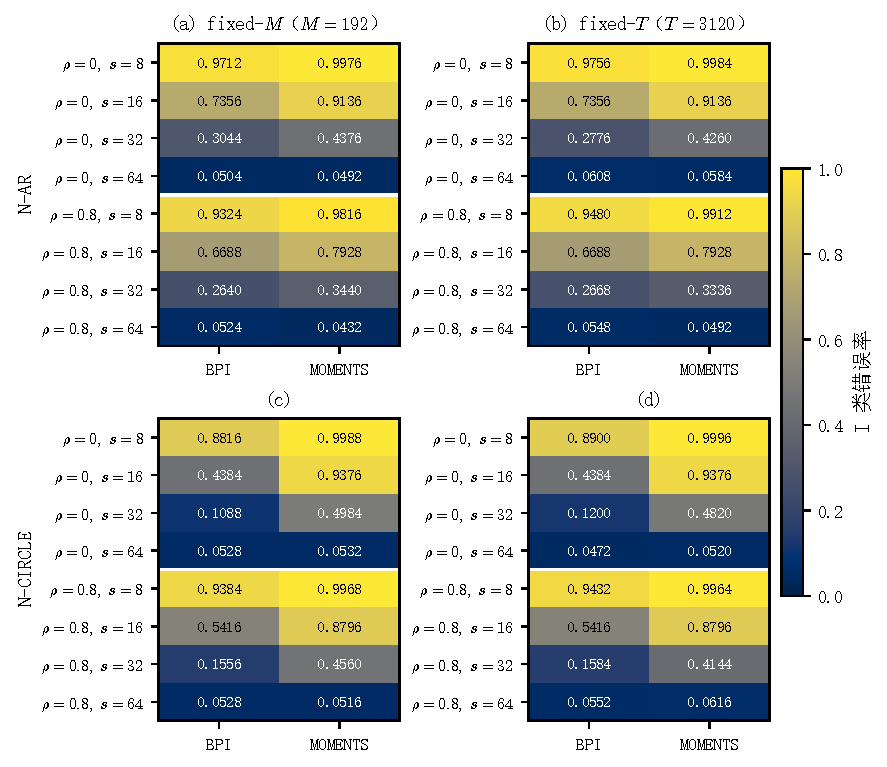
\includegraphics[width=0.92\textwidth]{../artifacts/figures/Figure3_M0_type1_surface.pdf}
\caption{M0（朴素置换）在两种预算制度下的有限样本 I 类错误率表面。两行分别为 N-AR 与 N-CIRCLE 数据生成过程，两列分别为固定窗口数（$M=192$）与固定观测长度（$T=3120$）；每面板行按 $\rho\times s$（$\rho\in\{0,0.8\}$，$s\in\{8,16,32,64\}$）排列，列为 BPI 与 MOMENTS 表示。色标 $[0,1]$，格内标注四位小数拒绝率。}\label{fig:m0-surface}
\end{figure}

\begin{figure}[ht]
\centering
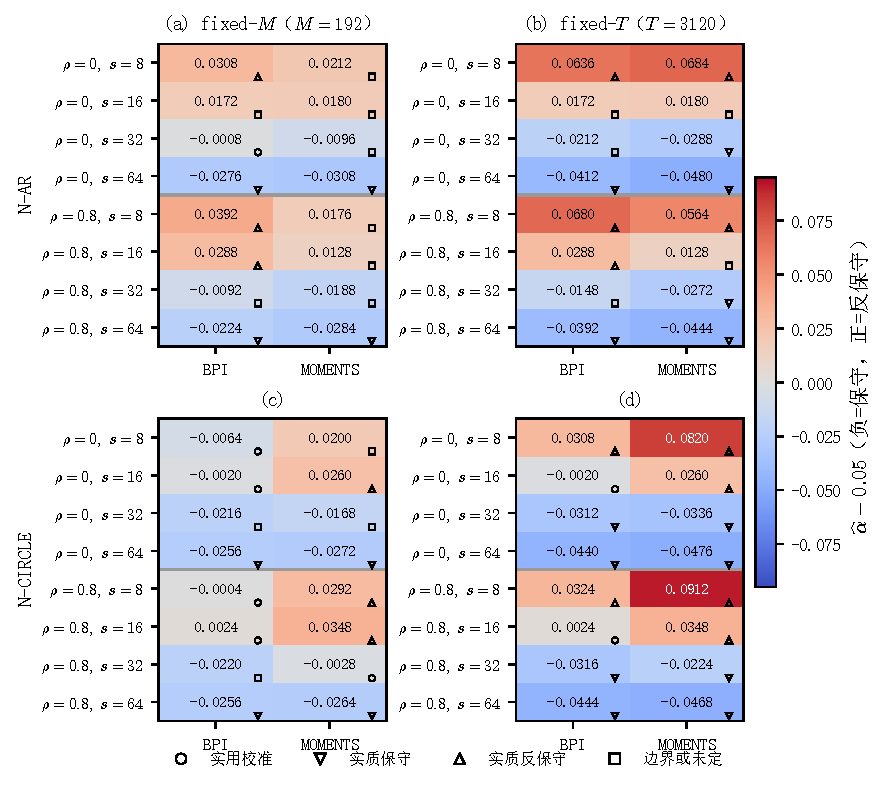
\includegraphics[width=0.92\textwidth]{../artifacts/figures/Figure4_M1_deviation_surface.pdf}
\caption{M1（依赖乘子法）在两种预算制度下的校准偏差 $\widehat\alpha-0.05$。两行分别为 N-AR 与 N-CIRCLE 数据生成过程，两列分别为固定窗口数与固定观测长度；每面板行按 $\rho\times s$（$\rho\in\{0,0.8\}$，$s\in\{8,16,32,64\}$）排列，列为 BPI 与 MOMENTS。色尺关于 0 对称，格内标注四位小数偏差；符号编码逐格 Wilson 判定（置于单元格右上角）：圆圈=实用校准，下三角=实质保守，上三角=实质反保守，方块=边界或未定。}\label{fig:m1-deviation}
\end{figure}

M0 的校准表现对窗口重叠高度敏感。BPI/M0 的逐格拒绝率介于 $0.0472$ 和 $0.9756$ 之间，MOMENTS/M0 介于 $0.0432$ 和 $0.9996$ 之间；对两种表示，20 个唯一重叠配置的 M0 均被判为实质反保守。M1 明显压缩了极端反保守性，其对应范围分别为 $0.0056$--$0.1180$ 和 $0.0020$--$0.1412$；对两种表示，8 个唯一非重叠配置的 M1 均被判为实质保守。在全部 56 个匹配的“配置--表示”组合中，M1 的拒绝率均低于 M0，但更低的拒绝率并不等同于更准确的校准。M1 的拒绝率同时分布在名义水平以下和以上，表明依赖感知乘子改变了校准图谱的形态，却未在所有有限样本配置中实现统一校准。

上述范围也说明，单一总体平均会掩盖具有相反方向的局部偏差。某些配置中的保守性和另一些配置中的反保守性可以在汇总后相互抵消，因此本文以逐格有效尺寸作为主要报告单位。

\subsection{逐格校准分类}\label{sec:h0-classify}

共有
\[
 28\text{（零假设配置）}\times2\text{（表示）}\times2\text{（方法）}=112
\]
个逐格评价单元。依据第~\ref{sec:estimands} 节的预设规则，表~\ref{tab:calibration}汇总四类校准状态。

\begin{table}[ht]
\centering
\footnotesize
\caption{逐格校准分类计数（每行 $n=28$）。完整 112 行拒绝率、Wilson 区间与分类结果见补充材料。}\label{tab:calibration}
\begin{tabular}{llcccc}
\toprule
表示 & 方法 & 实用校准 & 实质保守 & 实质反保守 & 边界/未定\\
\midrule
BPI & M0 & 7 (25.0) & 0 (0.0) & 20 (71.4) & 1 (3.6)\\
BPI & M1 & 5 (17.9) & 10 (35.7) & 7 (25.0) & 6 (21.4)\\
MOMENTS & M0 & 6 (21.4) & 0 (0.0) & 20 (71.4) & 2 (7.1)\\
MOMENTS & M1 & 1 (3.6) & 12 (42.9) & 7 (25.0) & 8 (28.6)\\
\bottomrule
\end{tabular}

\begin{minipage}{0.94\textwidth}
\vspace{0.4em}
\footnotesize 注：括号内为该类计数占 28 格的百分比。实用校准采用 90\% Wilson 区间完整落在等效带 $[0.035,0.065]$ 内，对应预设的实用等效性判据（两个单侧 5\% 判定等价于一个 90\% 双侧区间）；实质保守要求 95\% 区间完整位于实用带下方，实质反保守要求 95\% 区间完整位于实用带上方；边界/未定为既不满足实用校准、也不满足实质保守或实质反保守的剩余状态。上述计数为预设设计网格内的描述性分布，不构成方法在更广参数空间中的通过率。
\end{minipage}
\end{table}



对两种表示，M0 均有 $20/28$ 个配置被判为实质反保守，且没有配置被判为实质保守。M1 的分类则分散于实用校准、实质保守、实质反保守和边界未定四类：BPI/M1 中四类计数依次为 $5$、$10$、$7$ 和 $6$，MOMENTS/M1 中依次为 $1$、$12$、$7$ 和 $8$。这些计数描述预设设计网格内的有限样本分布，不应解释为方法在更广参数空间中的“通过率”。

\subsection{相邻格点的经验校准边界}\label{sec:h0-boundary}

题名中的“经验校准边界”对应有序设计维度上相邻格点发生校准状态变化的位置。以固定窗口数、N-AR、$\rho=0$、BPI 为例，依据逐格拒绝计数及第~\ref{sec:estimands} 节的 Wilson 判据，逐格状态随步长变化如下：$s=8,16,32$ 时 M0 均被判为实质反保守，$s=64$ 时转为实用校准，故 M0 的观测分类在步长 $32$ 与 $64$ 之间发生转换；M1 则随步长增加依次经历实质反保守（$s=8$）、边界或未定（$s=16$）、实用校准（$s=32$）与实质保守（$s=64$）。这里报告的是相邻格点的观测状态变化，不估计两点之间的连续临界步长，也不将其解释为连续参数域上的置信区间。完整的状态转换清单见补充材料 S1。

\subsection{主对比 P1--P3}\label{sec:h0-primary}

表~\ref{tab:primary}报告三个预先冻结主对比的点估计、边际 95\% basic 自助区间和 Holm 校正结果。按照第~\ref{sec:primary} 节的单侧阈值与多重性规则，三项对比均满足预设支持标准。

\begin{table}[ht]
\centering
\footnotesize
\caption{主对比 P1--P3 的效应量与推断结果。置信区间为边际 95\% basic 自助区间；原始单侧 bootstrap $p$ 值由 10,000 次整簇重采样的尾部计数按加一规则计算，随后对三项主对比实施 Holm 逐步校正，表中报告调整后 $p$ 值。}\label{tab:primary}
\begin{tabular}{llccccc}
\toprule
对比 & 估计量 & 点估计 & 阈值 & 超额效应 & 95\% basic CI & Holm $p$\\
\midrule
P1 & fixed-$M$：$s{=}16$ 减 $s{=}64$ & 0.5354 & 0.10 & 0.4354 & $[0.5210,0.5494]$ & 0.00030\\
P2 & fixed-$T$：$s{=}16$ 减 $s{=}64$ & 0.5330 & 0.10 & 0.4330 & $[0.5194,0.5462]$ & 0.00030\\
P3 & $0.05$ 减 M1 & 0.0266 & 0.01 & 0.0166 & $[0.0224,0.0308]$ & 0.00030\\
\bottomrule
\end{tabular}

\begin{minipage}{0.94\textwidth}
\vspace{0.4em}
\footnotesize 注：P1/P2 为 M0 拒绝率差（P1 固定窗口数，P2 固定观测长度），P3 为 $0.05$ 减 M1 拒绝率。三项尾部计数经真实 bootstrap 抽样核验均为 0，故原始 $p=1/10001\approx9.999\times10^{-5}$；经 Holm 逐步校正后三项调整 $p$ 均为 $3/10001\approx0.00030$。点估计与阈值之差为超额效应；正文按预设单侧阈值与多重性规则给出支持与否的表述，表中仅列统计量。
\end{minipage}
\end{table}



在固定窗口数制度下，$s=16$ 相对于 $s=64$ 的 M0 拒绝率差异，经两个数据生成过程等权平均后为 $0.5354$；在固定观测长度制度下，相应差异为 $0.5330$。两项区间的下界均远高于预设阈值 $0.10$，相对于该阈值的超额分别为 $0.4354$ 和 $0.4330$。因此，在两个预设数据生成过程、$\rho=0$ 和 BPI 表示的等权平均意义下，P1 与 P2 在各自预算制度下均超过预设的 $0.10$ 实质阈值，并通过 Holm 校正后的单侧判定。该结论不延伸为每一数据生成过程、每一依赖水平或每一表示下的必然规律。

P3 的估计为 $0.0266$，其 95\% 区间完整高于预设阈值 $0.01$。这表明在 $\rho=0$、$s=W=64$、固定 $M=192$ 的非重叠端，当前 M1 配置表现出可检测的保守偏差。该结果同时提示，依赖感知校准器在窗口不重叠时也需要接受有限样本验证。

\subsection{原序列依赖的效应修饰}\label{sec:h0-rho}

为避免将单一步长下的 $\rho$ 差异与重叠效应修饰混为一谈，次级分析采用步长对比的差。对数据生成过程 $g$、表示 $\varphi$ 和预算制度 $r$，定义
\begin{align}
 D_{g,\varphi}^{(r)}(\rho)
 &=\pi_{g,\rho,16,\mathrm{M0},\varphi}^{(r)}
  -\pi_{g,\rho,64,\mathrm{M0},\varphi}^{(r)},\\
 I_{g,\varphi}^{(r)}
 &=D_{g,\varphi}^{(r)}(0.8)-D_{g,\varphi}^{(r)}(0).
 \label{eq:rho-interaction}
\end{align}
其中 $I_{g,\varphi}^{(r)}$ 衡量原序列依赖对“$s=16$ 相对于 $s=64$”拒绝率差异的修饰。

描述性估计汇总于表~\ref{tab:rho-interaction}。正值表示 $\rho=0.8$ 放大步长对比，负值表示其缩小步长对比；修饰方向随数据生成过程和表示而变化，且不同条件的符号并不一致。由于该分析为次级描述，本文不据此提出原序列依赖具有统一单调作用的结论。

\begin{table}[ht]
\centering
\caption{原序列依赖对步长对比（$s=16$ 相对 $s=64$）的效应修饰 $I_{g,\varphi}^{(r)}$。正值表示 $\rho=0.8$ 放大步长对比，负值表示其缩小步长对比。}\label{tab:rho-interaction}
\begin{tabular}{llcc}
\toprule
表示 & 数据生成过程 & $I^{(M)}$ & $I^{(T)}$\\
\midrule
BPI & N-AR & $-0.0688$ & $-0.0608$\\
BPI & N-CIRCLE & $0.1032$ & $0.0952$\\
MOMENTS & N-AR & $-0.1148$ & $-0.1116$\\
MOMENTS & N-CIRCLE & $-0.0564$ & $-0.0676$\\
\bottomrule
\end{tabular}
\end{table}

\section{表示特异性的检出与定位性能}\label{sec:h1}

本节考察两类方向相反的备择。尺寸标准化功效按式\eqref{eq:size-standardized-power}计算：每个备择条件和表示均使用对应零假设配置的经验 0.95 临界值，从而减少参考分布松紧对表示比较的直接干扰。由于 M0 与 M1 使用相同的观测扫描统计量，每个“条件--表示”组合只产生一个尺寸标准化功效。场景层面的功效为四个预设条件 $(\rho,s)\in\{0,0.8\}\times\{16,64\}$ 的等权平均。

\subsection{形状变化}\label{sec:h1-shape}

在圆形到八字曲线的形状变化下，两种表示的平均尺寸标准化功效分别为
\[
 \widehat\beta_{\mathrm{BPI}}=1.00000,
 \qquad
 \widehat\beta_{\mathrm{MOMENTS}}=0.06203.
\]
定义场景差异为 BPI 减去 MOMENTS，则
\begin{equation}\label{eq:shape-power-diff}
 \Delta_{\mathrm{shape}}=0.93797,
 \qquad
 \text{95\% CI }[0.92969,0.94609].
\end{equation}
该区间为 2000 次保持条件配对结构的重采样所得 95\% 百分位自助区间。结果表明，在当前形状构造和固定表示参数下，BPI 保留了 MOMENTS 的一、二阶摘要未充分捕获的结构信息。该证据的适用范围限于本文定义的备择、窗口几何和表示实现，不能推广为拓扑表示对任意变化类型均占优势。

\subsection{均值平移反向对照}\label{sec:h1-mean}

在均值平移场景下，BPI 的平均尺寸标准化功效为 $0.05375$，MOMENTS 为 $1.00000$，因此
\begin{equation}\label{eq:mean-power-diff}
 \Delta_{\mathrm{mean}}=-0.94625,
 \qquad
 \text{95\% CI }[-0.95344,-0.93844].
\end{equation}
差异方向与形状变化场景相反。MOMENTS 直接包含窗口均值，因而在该构造中具有很高的检出能力；BPI 的尺寸标准化功效接近名义水平，说明固定持续强度表示对该平移信号的敏感性有限。

\begin{figure}[ht]
\centering
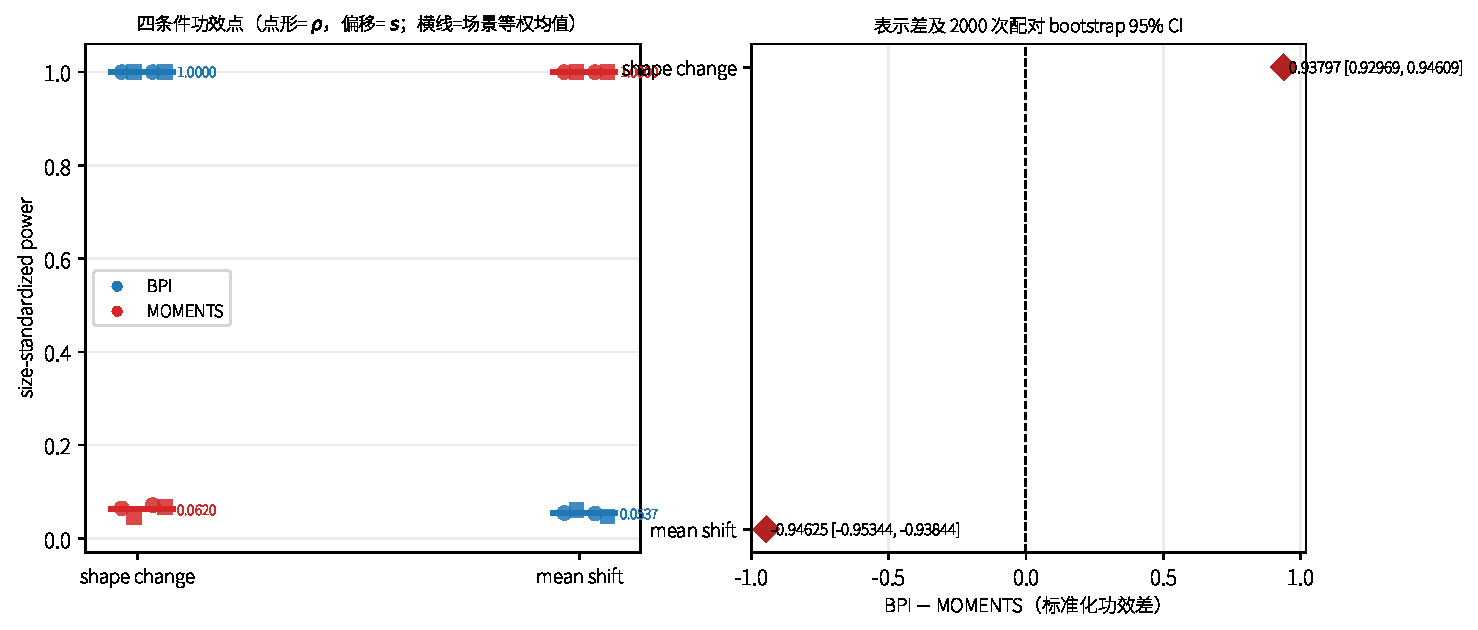
\includegraphics[width=0.95\textwidth]{../artifacts/figures/Figure5_H1_power_and_difference.pdf}
\caption{左：形状变化与均值平移下 BPI 与 MOMENTS 的条件级尺寸标准化功效。小点为四个预设条件之一（点形编码 $\rho$：圆圈 $\rho=0$，方块 $\rho=0.8$；水平偏移编码 $s$）；横线为场景等权平均功效。两个场景之间不使用连线，以避免暗示连续变化趋势。右：两个场景下 BPI 减去 MOMENTS 的功效差及 2000 次配对百分位自助 95\% 区间，零线表示无差异。右图区间只对应表示差异，不用作单个表示功效均值的误差条。完整 16 行条件级结果见补充材料。}\label{fig:h1-power}
\end{figure}

两个场景中出现的样本功效 $1.00000$ 表示 1600 次有限 Monte Carlo 重复在全部四个条件上的汇总结果，未构成总体功效恒等于 1 的概率保证。式\eqref{eq:shape-power-diff}与式\eqref{eq:mean-power-diff}共同支持表示选择性的结论：拓扑表示和矩表示保留了不同类型的变化信息，任何单一表示的检出能力均应结合备择结构加以评价。

\subsection{名义功效与尺寸标准化功效}\label{sec:h1-std}

直接以 $p\le0.05$ 计算的名义功效同时受到观测统计量和校准参考分布的影响。当对应零假设配置未达到点态实用校准时，名义功效可能因反保守性而被抬高，也可能因保守性而被压低。尺寸标准化功效改用匹配零假设统计量的经验临界值，使 BPI 与 MOMENTS 在各自零假设尺度上接受比较。该指标仍是条件化的有限样本量，不能消除表示维数、窗口参数和备择强度等设计因素的影响。

\subsection{定位误差与联合成功率}\label{sec:h1-localization}

位置估计由观测扫描曲线确定，按式\eqref{eq:location-map}映射回原始时间轴。由于变化在 $t=\lfloor T/2\rfloor$ 与 $t=\lfloor T/2\rfloor+1$ 之间发生，真实连续边界为
\begin{equation}\label{eq:true-location}
 \tau_{\mathrm{true}}=\left\lfloor\frac T2\right\rfloor+\frac12.
\end{equation}
本文报告无条件绝对误差
\[
 E_r=|\widehat\tau_r-\tau_{\mathrm{true}}|,
\]
原始尺度平均绝对误差 $R_1^{-1}\sum_rE_r$，以及归一化平均绝对误差
\begin{equation}\label{eq:normalized-mae}
 \operatorname{nMAE}
 =\frac1{R_1}\sum_{r=1}^{R_1}\frac{E_r}{T}.
\end{equation}
位置误差由观测统计量决定，因此对同一“条件--表示”组合，M0 与 M1 共享相同的 $\widehat\tau_r$。校准方法只通过拒绝事件影响联合成功率。对方法 $m\in\{\mathrm{M0},\mathrm{M1}\}$，定义
\begin{equation}\label{eq:joint-success}
 \widehat J_m
 =\frac1{R_1}\sum_{r=1}^{R_1}
 \mathbf1\left\{p_{r,m}\le0.05,\;
 |\widehat\tau_r-\tau_{\mathrm{true}}|\le\frac W2\right\}.
\end{equation}
漏检重复保留在式\eqref{eq:joint-success}的分母中，因此该量同时评价检出与定位。

表~\ref{tab:h1-power}以同一场景内四个预设条件的等权平均汇总功效、归一化定位误差和联合成功率。不同步长对应的 $T$ 不同，故正文采用式\eqref{eq:normalized-mae}保证条件间尺度可比；逐条件原始 MAE、匹配零假设临界值和对应 I 类错误率见补充材料。定位汇总由既有观测扫描结果重新计算，未改变或重跑 Monte Carlo 试次。

\begin{table}[ht]
\centering
\caption{同一场景内四个预设条件的等权描述性汇总。尺寸标准化功效使用各自匹配的零假设临界值；平均归一化 MAE 为无条件位置误差除以对应 $T$ 后的均值；联合成功率按式\eqref{eq:joint-success}分别计算。}\label{tab:h1-power}
\begingroup
\footnotesize
\setlength{\tabcolsep}{3.5pt}
\begin{tabular}{llccrr}
\toprule
场景 & 表示 & 检出能力 & 定位误差 & \multicolumn{2}{c}{检出--定位联合成功}\\
\cmidrule(lr){3-3}\cmidrule(lr){4-4}\cmidrule(lr){5-6}
 & & $\widehat\beta_{\mathrm{std}}$ & nMAE & M0 & M1\\
\midrule
形状变化 & BPI & 1.00000 & 0.00409 & 0.9839 & 0.9839\\
形状变化 & MOMENTS & 0.06203 & 0.20165 & 0.0144 & 0.0009\\
均值平移 & BPI & 0.05375 & 0.20255 & 0.0087 & 0.0011\\
均值平移 & MOMENTS & 1.00000 & 0.00330 & 0.9052 & 0.9052\\
\bottomrule
\end{tabular}
\endgroup
\end{table}



% 本稿未纳入自然数据案例；外部验证边界在讨论部分明确说明。

\section{讨论}\label{sec:discussion}

\subsection{重叠窗口引起的随机化单位错配}\label{sec:disc-validity}

本文的理论和模拟共同表明，重叠窗口带来的推断问题超出了“相关样本使有效样本量下降”的标量解释范围。窗口重用首先改变派生特征的联合分布：即使原始观测独立同分布，相邻特征仍可能共享大量底层随机变量，并形成随窗口距离变化的协方差。全局随机置换操作保留经验边际分布，却打散原始顺序中的滞后协方差，因此科学零假设下的“无变化”无法自动提供窗口层面的排列不变性。命题~\ref{prop:counterexample}给出了这一层级错配的有限样本反例，式\eqref{eq:permutation-fpc}则说明排列参考的条件变异只由经验边际量决定。该机制与依赖时间序列中置换检验需要附加有效性条件的既有理论一致\cite{RomanoTirlea2022}。

有效样本量仍可作为特定线性统计量的直观概括。例如，$W=64$、$s=16$、$M=192$ 时，窗口均值的方差比约为 $3.974$。然而，窗口均值的方差比可以解释特定线性统计量的变异变化，但不能直接决定一般高维最大扫描的参考分布及其拒绝率。本文因此对完整检验逐条件开展模拟评价。

\subsection{双预算视角与条件化校准图谱}\label{sec:disc-surface}

固定窗口数和固定观测长度回答不同的条件问题。前者保持扫描序列长度 $M$ 不变，步长变化同时改变原始观测长度；后者保持 $T$ 不变，步长变化同时改变窗口数。两种制度均无法单独隔离所有设计因素，但它们提供了互补的预算视角。P1 与 P2 在两个预设数据生成过程的等权平均下均超过预设实质阈值，说明严重失校准并非某一种预算制度的偶然产物。相应结论仍应限定于本文的 $W$、步长网格、数据生成过程和表示实现。

校准图谱的概念还强调，汇总平均不能替代逐格有效性判断。朴素置换下，BPI 与 MOMENTS 的拒绝率范围分别为 $0.0472$--$0.9756$ 和 $0.0432$--$0.9996$。依赖乘子校准下，相应范围分别为 $0.0056$--$0.1180$ 和 $0.0020$--$0.1412$。将条件间的保守性与反保守性合并，可能得到接近 $0.05$ 的总体均值，同时掩盖局部严重失真。因此，本文将逐格拒绝率、Wilson 区间和预设实用等价带作为主要证据。该分类依赖 Monte Carlo 样本量和等价带宽度，属于操作性有限样本判据。

\subsection{依赖乘子校准的改善与局限}\label{sec:disc-dmb}

M1 在多数重叠配置中大幅降低了 M0 的极端反保守性，说明相关乘子在参考过程中引入了预设相关结构。不过，M1 仍同时产生实质保守和实质反保守配置。一般 dependent wild bootstrap 或依赖乘子理论主要针对特定均值、光滑函数或经验过程\cite{Shao2010,BucherKojadinovic2016}：Shao 的 dependent wild bootstrap 面向平稳序列的部分和近似，B{\"u}cher 与 Kojadinovic 的依赖乘子则针对强混合经验 copula 过程，二者均在各自函数类内给出渐近有效性。这些理论为窗口特征序列提供了渐近分析的起点，但均未提供本文完整 BPI 最大扫描在当前样本规模和固定带宽规则下的有限样本校准保证；其适用性仍需针对本文的局部映射、扫描泛函与带宽规则逐项验证。

当前带宽规则也有助于解释非重叠端的保守性。即使 $s=W$，式\eqref{eq:dmb-bandwidth}中的 $\lceil M^{1/3}\rceil$ 仍使 $b>1$；以 P3 的固定 $M=192$ 配置为例，$b=6$，相关乘子不会退化为独立乘子。P3 检出的保守偏差与这一结构相容，但本文没有进一步分解带宽、桥接和高维特征谱各自的贡献。后续研究可针对窗口依赖尺度推导步长适配的乘子协方差，或在原始时间轴上实施块重采样并重新构造全部窗口特征。此类扩展需要新的理论和独立确认实验。

\subsection{表示敏感性与校准有效性}\label{sec:disc-representation}

形状变化和均值平移中的功效反转说明，表示选择决定了观测统计量能够保留何种信号。BPI 在圆形到 8 字形曲线的变化中具有很高的尺寸校正功效，MOMENTS 在均值平移中具有对应优势。尺寸校正临界值减少了零假设校准松紧对这一比较的直接影响，因此结果更接近表示层面的信号选择性。与此同时，该比较仍受窗口宽度、表示超参数、变化强度和有限样本设计约束。

表示敏感性与校准有效性应作为两个不同评价维度。信息不足的表示难以通过更准确的校准获得高功效；失真的参考分布也会使信息充分的表示产生错误的显著性判断。两者在有限样本下还可能通过维数、依赖谱和乘子带宽发生交互，本文没有假设其统计独立或严格正交。定位结果进一步显示，观测扫描曲线决定无条件位置误差，校准方法通过拒绝事件影响“检出且定位成功”的联合概率；这两个指标回答的统计问题需要保持区分。

\subsection{实践含义}\label{sec:disc-practice}

对采用重叠窗口的拓扑变化检测，本文给出三条操作建议：\begin{enumerate}\item 将窗口视为派生统计单位，而非因原始观测独立同分布就直接实施窗口级全局随机置换；校准单位应显式声明。\item 方法报告应明确窗口宽度、步长、原始长度、窗口数与校准单位，并在与实际管线匹配的零假设下逐条件评估 I 类错误率，而非依赖单一汇总平均。\item 固定观测预算与固定窗口数对应不同部署约束，其结论不宜互相替代；依赖感知重采样可作为更合理的参考起点，但其带宽与有限样本行为仍需针对具体表示与扫描统计量验证。\end{enumerate}

\subsection{研究局限}\label{sec:limitations}

本文的结论具有以下局限。
\begin{enumerate}
\item BPI 网格、核宽、尺度上界、同调通道和 MOMENTS 构造均保持固定；本文未系统遍历表示超参数，也未研究特征维数与校准行为之间的敏感性。
\item 零假设仅包含 N-AR 与 N-CIRCLE 两类合成过程，主要结论依赖两个过程的等权设计；更广的非高斯、长记忆、异方差和非平稳零模型尚待检验。
\item 备择仅包括一种形状变化和一种均值平移。形状构造匹配单时点边际均值与协方差，但没有匹配完整滞后联合分布或二阶过程。
\item M1 是冻结的依赖感知参考方法，本文没有为完整 BPI 最大扫描建立新的有限样本或渐近有效性定理，当前带宽规则也未针对每个步长进行最优选择。
\item 逐格校准分类为点态判断，依赖预设等价带和 Monte Carlo 精度，不提供整个设计域上的同时保证。
\item 本稿未纳入自然数据或独立外部数据集，外部有效性主要由合成设计的覆盖范围限定。
\item 本文研究单一变点的最大扫描，尚未处理多变点递归、停止规则及相应的族错误率控制。
\end{enumerate}

\section{结论}\label{sec:conclusion}

本文评估了基于持续同调特征的变点检验在重叠滑动窗口下的有限样本校准。窗口均值反例说明，原始观测独立同分布不能自动保证派生窗口序列具有交换性。在所考察的设计网格内，朴素置换在两种表示的全部重叠配置中均表现为实质反保守；依赖乘子法普遍降低拒绝率，但在非重叠配置中表现为实质保守，未实现逐条件统一校准。原序列依赖对步长对比的影响随数据生成过程和表示变化。形状备择和整体平移负对照进一步表明，持续同调表示保留的结构信息及其不变性，需要与下游检验的误报控制分开解释。上述结论为当前固定实现提供有限样本参照，其范围由生成过程、窗口设计、表示参数和校准规则共同限定。


\section*{Data and Code Availability}
复现本文结果的代码、配置、种子清单、完整逐格数据与补充材料由仓库 \url{https://github.com/dw0911/owtda-calibration} 提供。本稿对应 git 标签 \texttt{v1.1.1-paper}；全部合成数据均由该版本代码与固定随机种子生成，不依赖外部数据归档，独立数据 DOI 尚在建立中，未作为已提供材料列出。补充材料 S5 给出代码入口与复现步骤。

\bibliographystyle{unsrt}
\bibliography{bibliography}
\end{document}
"`。
\newif\ifstrictfigures
\strictfiguresfalse
\IfFileExists{STRICT.tex}{\strictfigurestrue}{}

\let\OriginalIncludeGraphics\includegraphics
\RenewDocumentCommand{\includegraphics}{O{} m}{%
  \IfFileExists{#2}{%
    \OriginalIncludeGraphics[#1]{#2}%
  }{%
    \ifstrictfigures
      \PackageError{owtda-paper}{Strict build: missing figure `\detokenize{#2}'}%
        {The strict build (paper/STRICT.tex present) requires every figure to exist.}%
    \else
      \begin{minipage}[c][4.2cm][c]{0.82\linewidth}
        \centering\small 图件缺失：\texttt{\detokenize{#2}}
      \end{minipage}%
    \fi
  }%
}

\title{重叠窗口拓扑扫描的有限样本校准边界\\\large Finite-Sample Calibration Boundaries for Topological Change-Point Scans with Overlapping Windows}
\author{
  王平\textsuperscript{1}\quad
  黄盛南\textsuperscript{1}\quad
  张晓媛\textsuperscript{1,*}\\[2mm]
  \small $^1$河北金融学院统计与数据科学学院\\[1mm]
  \small 通讯作者：张晓媛，\texttt{zxy0407010229@163.com}
}
\date{2026年9月}

\begin{document}
\maketitle

\begin{abstract}
基于持续同调的时间序列变点检验可利用滑动窗口提取局部结构特征，但窗口共享观测引起的依赖可能使随机置换参考分布失真。本文考察固定持续图向量表示与最大扫描所构成检验的有限样本校准。首先，以高斯窗口均值构造反例，说明原始观测独立同分布仍不足以保证派生窗口序列的交换性。随后，在固定窗口数与固定原始观测长度两种设计下，对 28 个零假设配置比较无约束窗口级随机置换与依赖乘子自助法，并以均值--协方差特征作为非拓扑对照。在名义显著性水平 0.05 下，对每种表示，20 个重叠配置均表现为实质反保守，持续同调表示的经验拒绝率最高为 0.9756。依赖乘子法在全部匹配配置中降低拒绝率，但对每种表示，8 个非重叠配置均表现为实质保守；原序列依赖对步长对比的修饰方向随生成过程与表示变化。低阶矩匹配的圆形到 8 字形曲线备择下，两类表示的尺寸校正功效分别为 1.0000 和 0.0620；整体平移负对照则呈相反结果，与距离型持续同调的平移不变性一致。结果表明，当前实现的校准表现具有明确的条件依赖性，降低拒绝率不能等同于恢复名义校准，表示的信号敏感性与检验的误报控制应分别评价。

\noindent\textbf{关键词}：持续同调；变点检测；重叠滑动窗口；交换性；有限样本校准。

\end{abstract}

\section*{Abstract}
Change-point tests based on persistent homology use sliding windows to extract local structural features, but dependence induced by shared observations can distort random-permutation reference distributions. This study examines the finite-sample calibration of a test combining a fixed vector representation of persistence diagrams with a maximum scan statistic. A Gaussian window-mean counterexample first shows that independent and identically distributed raw observations do not ensure exchangeability of the derived window sequence. Naive unrestricted window-level permutation and a dependent multiplier bootstrap are then evaluated under fixed-window-count and fixed-observation-length designs across 28 null configurations, with mean--covariance features as a non-topological comparator. At the nominal level of 0.05, all 20 overlapping-window configurations are classified as materially anti-conservative for each representation; the empirical rejection rate for the persistent-homology representation reaches 0.9756. The multiplier procedure lowers rejection rates in every matched configuration, but all eight non-overlapping configurations are materially conservative for each representation. The effect of serial dependence on the stride contrast varies across generators and representations. Under a circle-to-figure-eight alternative with matched first and second marginal moments, size-adjusted powers are 1.0000 and 0.0620 for the persistent-homology and moment representations, respectively. A mean-shift negative control reverses this ordering, consistently with the translation invariance of distance-based persistent homology. These results demonstrate condition-dependent calibration for the studied implementation: lower rejection rates do not necessarily imply nominal calibration, and representation sensitivity and Type-I error control require separate evaluation.

\noindent\textbf{Keywords}: persistent homology; change-point detection; overlapping sliding windows; exchangeability; finite-sample calibration.


\section{引言}\label{sec:intro}

\subsection{研究背景与统计问题}\label{sec:intro-bg}

时间序列的结构变化既可能表现为均值、方差等低阶统计量的改变，也可能表现为局部轨迹几何、周期结构或状态空间形状的改变。滑动窗口和时延嵌入为后一类信号提供了局部化表示：每个时间片段被转换为点云，持续同调进一步从多尺度上提取连通分支和环等结构信息。相关理论奠定了滑动窗口持久性分析的基础\cite{PereaHarer2015}，持续图像等有限维表示则使持续图能够进入统计扫描和机器学习程序\cite{Adams2017}。近年来，拓扑摘要已被用于离线变点检测、在线监测及依赖序列中的结构异常识别\cite{IslambekovYuvarajGel2020,ZhengMakXieXie2023,ChazalLevrardRoyer2024,NieYue2026}。

为提高候选变点的扫描密度，实际分析常取步长 $s$ 小于窗口宽度 $W$。此时，相邻窗口共享原始观测，窗口特征序列由此形成局部依赖。设第 $i$ 个窗口经固定映射得到特征 $Y_i$。对全部窗口顺序实施置换时，有限样本精确性通常依赖联合分布对排列群保持不变，即
\begin{equation}\label{eq:intro-exchangeability}
 (Y_1,\ldots,Y_M)\overset{d}{=}(Y_{\pi(1)},\ldots,Y_{\pi(M)}),
 \qquad \forall\,\pi\in\mathfrak S_M.
\end{equation}
独立同分布是满足该条件的一种充分情形，排列操作直接要求的条件则是窗口特征层面的联合交换性。窗口共享观测可诱发局部依赖，但特定映射是否具有交换性取决于其联合分布；平稳性、边际同分布以及原始序列的独立同分布性质，在窗口重叠时均不足以一般性地推出式\eqref{eq:intro-exchangeability}。由此形成本文关注的统计错配：科学零假设定义在原始过程的“无变化”层面，置换校准所需的对称性定义在派生窗口特征的联合分布层面。依赖时间序列中的置换理论同样表明，未经修正的排列参考分布可能无法维持名义检验水平\cite{RomanoTirlea2022}；随机排列检验的有限样本有效性还需相应的群不变性条件\cite{HemerikGoeman2018}。

本文考察一种基于持续同调特征的变点检验：每个局部时间窗口映射为点云，点云经持续同调及固定向量化形成特征序列，再通过标准化部分和的最大值检测前后特征均值差异。持续同调决定检验保留的结构信息，重采样程序决定统计量的参考分布。本文重点评价窗口重叠对后者有限样本校准的影响，并以均值--协方差特征作为非拓扑对照。

\subsection{相关工作与研究缺口}\label{sec:intro-lit}

与本文相关的研究可概括为三条脉络。第一类工作研究滑动窗口嵌入、持续同调及持续图向量化，为局部时间片段的拓扑表示提供方法基础\cite{PereaHarer2015,Adams2017}，其关注点主要在于表示的稳定性与可解释性，而未系统考察重叠窗口下推断有效性的有限样本校准。第二类工作将拓扑摘要引入离线或在线变化检测，并显式处理时间依赖与误报控制：文献\cite{NieYue2026}已经分析重叠窗口下的依赖继承，并利用移动块自助法校准在线监测控制限；其它近邻工作则聚焦表示对结构变化的辨识能力及特定检测程序的性能\cite{IslambekovYuvarajGel2020,ZhengMakXieXie2023,ChazalLevrardRoyer2024}。本文沿用这一研究背景，固定表示、离线最大扫描和校准规则，比较两种观测预算下的零假设拒绝率与经验分类。第三类工作研究依赖数据下的置换、dependent wild bootstrap 与依赖乘子自助法，说明时间依赖会改变随机化参考分布，并为若干均值、光滑函数或经验过程问题建立渐近理论\cite{RomanoTirlea2022,Shao2010,BucherKojadinovic2016}。这些理论为窗口特征序列提供了渐近分析的起点，但其适用性仍需针对本文所用的局部映射、扫描泛函与带宽规则逐项验证。

这些结果尚未提供本文实现的具体有限样本保证：重叠局部窗口依次经过点云映射、持续同调向量化和最大扫描后，朴素置换会产生多大程度的有限样本尺寸失真；该失真如何随重叠程度、原序列依赖、观测预算和表示类型变化；依赖感知校准能够在哪些条件下减弱失真，又会在哪些条件下表现为保守或残留反保守。本文不以非线性变换本身主张该管线脱离既有理论框架，也不从渐近一致性推定当前样本规模下的名义尺寸控制，而以固定实现和预设设计网格上的有限样本校准偏差及其条件变化为考察重点。本文将条件组合 $\theta$ 下的有效检验水平记为 $\alpha_{\mathrm{eff}}(\theta)$，并将映射 $\theta\mapsto\alpha_{\mathrm{eff}}(\theta)$ 称为预设离散设计网格上的条件化有限样本校准图谱。本文不估计连续参数空间中的解析边界；“经验校准状态转换”仅指有序设计维度（主要为步长或重叠率）上相邻格点发生校准分类变化的位置。该图谱属于有限样本、点态和设计域内的刻画，不提供全参数空间的统一保证。

\subsection{研究目标与贡献}\label{sec:intro-contrib}

本文的主要贡献是对固定持续同调变点检验开展条件化有限样本校准评价：在两种预算设计和 28 个唯一零假设配置上，报告朴素置换与依赖乘子的拒绝率、区间及经验分类，并量化两种预算下重叠与非重叠条件之间的预设对比。机制分析通过一般局部映射的依赖继承和窗口均值反例说明交换性风险；备择分析通过低阶矩匹配的形状构造与整体平移负对照，解释固定表示的信号敏感性及不变性。理论推导、经验评价与构造对照分别承担机制、实际表现和解释功能。

全文其余部分安排如下：第~\ref{sec:method} 节定义重叠窗口特征、两类表示、最大扫描统计量及校准方法；第~\ref{sec:theory} 节分析有限依赖、交换性失效与方差机制；第~\ref{sec:protocol} 节说明评价对象和实验设计；第~\ref{sec:h0} 节报告零假设下的有限样本校准结果；第~\ref{sec:h1} 节分析备择下的检出与定位性能；第~\ref{sec:discussion} 节讨论方法含义、适用范围与局限；第~\ref{sec:conclusion} 节总结全文。

\section{基于持续同调特征的变点检验}\label{sec:method}

图~\ref{fig:flow}给出整体流程与统计冲突的来源：窗口是随机化单位，但重叠使原始观测被多个随机化单位共享。后续小节依次定义窗口构造、两种表示、最大扫描统计量与两种校准方法。

\begin{figure}[tbp]
\centering
\begin{subfigure}[t]{0.92\linewidth}
\centering
\caption{统计推断主流程}\label{fig:flow-a}
% 图 1(a)：重叠窗口拓扑扫描与校准的统计推断主流程（横向）。
% 依赖 main.tex 中定义的 flowblue/flowfill/m0fill/m1fill 配色与 tikz 库。
\begin{tikzpicture}[
  font=\footnotesize,
  box/.style={draw=flowblue, fill=flowfill, rounded corners=2pt,
              align=center, inner xsep=6pt, inner ysep=5pt, line width=0.6pt},
  arr/.style={-{Stealth[length=2.4mm]}, flowblue, line width=0.6pt},
]
\node[box] (raw) {原始序列\\ $X_1,\ldots,X_T$};
\node[box, right=4mm of raw] (win) {重叠滑动窗口\\ $I_1,\ldots,I_M$};
\node[box, right=4mm of win] (pc) {窗口点云\\ $P_i$};
\node[box, fill=m0fill, above right=3mm and 4mm of pc] (bpi) {持续同调 $\to$ 持续图\\ $\to$ BPI（800 维）};
\node[box, fill=m1fill, below right=3mm and 4mm of pc] (mom) {MOMENTS\\ （5/9 维）};
\coordinate (mid1) at ($(bpi.south east)!0.5!(mom.north east)$);
\node[box, right=4mm of mid1] (scan) {最大扫描\\ $T_M,\ \hat k$};

\node[box, fill=m0fill, below=15mm of scan, xshift=-19mm] (m0) {M0：全局随机置换重采样\\ $T_M^{*(1\ldots B)}$};
\node[box, fill=m1fill, below=15mm of scan, xshift=19mm] (m1) {M1：相关乘子重采样\\ （近似局部依赖）};

\coordinate (mid2) at ($(m0.south)!0.5!(m1.south)$);
\node[box, below=6mm of mid2] (ref) {参考分布 $\{T_M^*\}$\\ ＋ 观测 $T_M$};
\node[box, left=6mm of ref] (pv) {Monte Carlo\\ $p$ 值};
\node[box, left=6mm of pv] (dec) {拒绝 / 不拒绝\\ ＋ 位置估计 $\hat k$};

\draw[arr] (raw) -- (win);
\draw[arr] (win) -- (pc);
\draw[arr] (pc) -- (bpi);
\draw[arr] (pc) -- (mom);
\draw[arr] (bpi) -- (scan);
\draw[arr] (mom) -- (scan);
\draw[arr] (scan) -- (m0);
\draw[arr] (scan) -- (m1);
\draw[arr] (m0) -- (ref);
\draw[arr] (m1) -- (ref);
\draw[arr] (ref) -- (pv);
\draw[arr] (pv) -- (dec);
\end{tikzpicture}

\end{subfigure}

\vspace{1.2em}

\begin{subfigure}[t]{0.85\linewidth}
\centering
\caption{窗口重叠与共享观测机制}\label{fig:flow-b}
% 图 1(b)：窗口重叠与共享观测 + 全局随机置换破坏邻接。
\begin{tikzpicture}[
  font=\small,
  obs/.style={circle, draw=flowblue, fill=white, inner sep=1.2pt, line width=0.5pt},
  shared/.style={circle, draw=sharedred, fill=sharedred!25, inner sep=1.7pt, line width=0.6pt},
]
% 时间轴与观测
\foreach \i in {1,...,8} { \coordinate (X\i) at (\i, 0); }
\draw[flowblue, line width=0.5pt] (0.5,0) -- (8.5,0);
\foreach \i in {1,7,8} { \node[obs] at (X\i) {}; }
\foreach \i in {2,3,4,5,6} { \node[shared] at (X\i) {}; }
\foreach \i in {1,...,8} { \node[below=1.5mm, font=\footnotesize] at (X\i) {$X_{\i}$}; }

% 四个窗口（各覆盖 4 个连续观测，相邻窗口共享 3 个观测；与下方全局随机置换的 4 个窗口一致）
\draw[winblue, line width=1.3pt] (1,1.9) -- (4,1.9);
\draw[winblue, line width=0.8pt] (1,1.68) -- (1,2.12);
\draw[winblue, line width=0.8pt] (4,1.68) -- (4,2.12);
\node[right=1mm, font=\footnotesize] at (4,1.9) {窗口1};

\draw[winblue, line width=1.3pt] (2,1.35) -- (5,1.35);
\draw[winblue, line width=0.8pt] (2,1.13) -- (2,1.57);
\draw[winblue, line width=0.8pt] (5,1.13) -- (5,1.57);
\node[right=1mm, font=\footnotesize] at (5,1.35) {窗口2};

\draw[winblue, line width=1.3pt] (3,0.8) -- (6,0.8);
\draw[winblue, line width=0.8pt] (3,0.58) -- (3,1.02);
\draw[winblue, line width=0.8pt] (6,0.58) -- (6,1.02);
\node[right=1mm, font=\footnotesize] at (6,0.8) {窗口3};

\draw[winblue, line width=1.3pt] (4,0.25) -- (7,0.25);
\draw[winblue, line width=0.8pt] (4,0.03) -- (4,0.47);
\draw[winblue, line width=0.8pt] (7,0.03) -- (7,0.47);
\node[right=1mm, font=\footnotesize] at (7,0.25) {窗口4};

% 共享标注（置于窗口条上方）
\node[sharedred, font=\footnotesize] at (4.5,2.6) {共享观测（相邻窗口重叠 $W-s$ 个观测）};

% 全局随机置换示意（方块组居中于时间轴中心 x≈4.5，避免视觉偏左）
\foreach \i/\n in {1/1,2/2,3/3,4/4} {
  \node[draw=flowblue, fill=flowfill, minimum size=7mm, font=\footnotesize] at ({2.25+0.9*\i}, -2.3) {\n};
}
\node[left=2mm, font=\footnotesize] at (3.15,-2.3) {原始窗口序};
\foreach \i/\n in {1/3,2/1,3/4,4/2} {
  \node[draw=flowblue, fill=flowfill, minimum size=7mm, font=\footnotesize] at ({2.25+0.9*\i}, -3.8) {\n};
}
\node[left=2mm, font=\footnotesize] at (3.15,-3.8) {随机置换后};
\draw[-{Stealth[length=2mm]}, sharedred, line width=0.6pt] (3.6,-2.7) -- (3.6,-3.4);
\node[sharedred, right=2mm, font=\footnotesize] at (3.6,-3.05) {窗口级邻接被破坏};
\end{tikzpicture}

\end{subfigure}

\caption{基于持续同调特征的变点检验与校准流程。(a) 原始序列经重叠窗口映射为窗口点云，再分别经持续同调—向量化分支得到 BPI、经均值—协方差分支得到矩表示 MOMENTS，进入最大扫描得到检验统计量 $T_M$ 与位置估计 $\hat k$；随后 M0 无约束窗口级随机置换重采样、M1 相关乘子重采样分别构造参考分布，并通过 Monte Carlo $p$ 值形成拒绝决策。(b) 重叠机制：相邻窗口共享原始观测（红色），无约束窗口级随机置换重排窗口顺序时原有邻接被破坏，这是后文交换性失效机制的直观来源。}\label{fig:flow}
\end{figure}

\subsection{窗口构造与局部点云}\label{sec:windows}

给定观测序列 $X_1,\ldots,X_T$，取窗口宽度 $W$ 和步长 $s$，并令
\begin{equation}\label{eq:windows}
 a_i=(i-1)s+1,\qquad
 I_i=\{a_i,\ldots,a_i+W-1\},\qquad
 M=\left\lfloor\frac{T-W}{s}\right\rfloor+1.
\end{equation}
本文考虑 $1\le s\le W$，相邻窗口的名义重叠率为 $1-s/W$。对于二维观测，窗口点云直接定义为 $P_i=\{X_t:t\in I_i\}$。对于标量观测，在每个窗口内部构造三维时延点云
\begin{equation}\label{eq:delay-cloud}
 P_i=\bigl\{(X_t,X_{t+3},X_{t+6}):t=a_i,\ldots,a_i+W-7\bigr\},
\end{equation}
因而时延坐标不会跨越窗口边界。点云在计算持续同调前按固定规则进行精确去重；所有坐标尺度、网格、核宽和截断参数均预先设定，且不利用整条序列共同估计的自适应参数。该局部性条件将在第~\ref{sec:theory} 节用于界定窗口特征的依赖范围。

\subsection{固定网格持续强度表示}\label{sec:bpi}

对每个点云 $P_i$，在系数域 $\mathbb F_2$ 上按欧氏距离计算 Vietoris--Rips 持续同调，并保留 0 维和 1 维同调通道中有限且寿命为正的 birth--death 对。过滤采用边长阈值的直径约定：单形 $\sigma$ 的过滤值为其顶点间最大欧氏距离，即 $\operatorname{diam}(\sigma)$；尺度 $\varepsilon$ 下纳入所有满足 $\operatorname{diam}(\sigma)\le\varepsilon$ 的单形，即 $\operatorname{VR}_\varepsilon(P)=\{\sigma\subseteq P:\operatorname{diam}(\sigma)\le\varepsilon\}$。过滤不设数据驱动的截断上限，持续图坐标直接以欧氏距离尺度报告。由于有限欧氏点云的 Vietoris--Rips 过滤在过滤值达到点云直径时形成完全复形，所有 1 维同调类在此时均已消亡，仅最后一个 0 维连通分量的 death 为 $\infty$；实现中只丢弃该显式无限 death 分量，其余有限类全部保留。相关计算框架和有限维表示可分别参见\cite{Bauer2021,Adams2017}。

记 $K_i(\varepsilon)=\operatorname{VR}_\varepsilon(P_i)$。随过滤尺度 $\varepsilon$ 增大，复形形成嵌套序列 $K_i(\varepsilon)\subseteq K_i(\varepsilon')$（$\varepsilon\le\varepsilon'$）。零维同调记录连通分支，一维同调记录未被二维单形填充的独立循环；贝蒂数 $\beta_q(K_i(\varepsilon))=\dim H_q(K_i(\varepsilon);\mathbb F_2)$ 表示该尺度下相应同调空间的维数。持续同调进一步记录这些类随过滤尺度的出现与消失，由持续图中的 $(b,d)$ 概括，其中 $b$ 与 $d$ 分别为出生尺度与消亡尺度，$d-b$ 是过滤尺度上的寿命，而非真实时间轴上的持续时长。记第 $q\in\{0,1\}$ 个同调通道的持续图为
\[
 \mathcal D_i^{(q)}=\{(b_{ij}^{(q)},d_{ij}^{(q)})\}_j.
\]
给定场景固定的尺度上界 $c$，将每个有限持续图点转换为归一化 birth--lifetime 坐标。尺度上界 $c$ 仅用于该坐标缩放与截断，不用于提前终止过滤；过滤本身以 $+\infty$ 为阈值完整计算。
\begin{equation}\label{eq:bpi-normalization}
 u_{ij}^{(q)}=\min\left(\frac{b_{ij}^{(q)}}{c},1\right),\qquad
 v_{ij}^{(q)}=\min\left(\frac{d_{ij}^{(q)}-b_{ij}^{(q)}}{c},1\right).
\end{equation}
令 $\Delta=1/20$、$g_r=(r+1/2)\Delta$（$r=0,\ldots,19$）以及 $\sigma=0.05$。第 $q$ 个通道在网格中心 $(g_r,g_\ell)$ 上的持续强度坐标定义为
\begin{equation}\label{eq:bpi}
 Z_{i,r\ell}^{(q)}
 =\frac{\Delta}{2\pi\sigma^2}
 \sum_j v_{ij}^{(q)}
 \exp\left\{-\frac{(g_r-u_{ij}^{(q)})^2+(g_\ell-v_{ij}^{(q)})^2}{2\sigma^2}\right\}.
\end{equation}
每个同调通道产生 $20\times20=400$ 个坐标。按 0 维、1 维同调通道的顺序向量化并连接，再除以 $\sqrt 2$（该缩放使两个同调通道对总平方距离的贡献取等权平均），得到 800 维特征。此处涉及三类维数：同调维数 $q\in\{0,1\}$、点云所在空间维数 $d\in\{2,3\}$ 以及向量表示维数 $p=800$；$800$ 维特征不意味着本文研究了 $800$ 维拓扑。
\begin{equation}\label{eq:bpi-vector}
 Y_i^{\mathrm{BPI}}
 =\frac{1}{\sqrt2}
 \begin{bmatrix}
   \operatorname{vec}(Z_i^{(0)})\\
   \operatorname{vec}(Z_i^{(1)})
 \end{bmatrix}.
\end{equation}
空通道记为 400 维零向量。N-AR 时延点云取 $c=6$，圆形模型及其备择取 $c=2.5$。本文将每个持续图中以寿命加权的高斯核表面在固定网格中心进行评价，并将两个同调通道的结果拼接为向量，沿用实现标识 BPI。该表示与持续图像共享“持续图--加权核表面--有限维表示”的思路，但其离散化采用网格中心采样，区别于逐像素积分\cite{Adams2017}。BPI 仅标识本文的固定实现，不另行宣称一种标准 Betti 不变量，也不构成对随机持续图总体强度密度的估计\cite{WuKimRinaldo2023}。

\subsection{矩表示}\label{sec:moments}

为构造低阶统计摘要作为对照，设窗口点云为 $P_i=\{x_{ij}\}_{j=1}^{n_i}\subset\mathbb R^d$，并定义
\begin{equation}\label{eq:moments}
 \bar x_i=\frac1{n_i}\sum_{j=1}^{n_i}x_{ij},\qquad
 S_i=\frac1{n_i}\sum_{j=1}^{n_i}(x_{ij}-\bar x_i)(x_{ij}-\bar x_i)^\top.
\end{equation}
MOMENTS 特征依次连接均值、协方差对角元以及按固定字典序排列的 $\sqrt2(S_i)_{ab}$（$a<b$）：
\begin{equation}\label{eq:moments-vector}
 Y_i^{\mathrm{MOM}}
 =\bigl(\bar x_i^\top,(S_i)_{11},\ldots,(S_i)_{dd},
 \{\sqrt2(S_i)_{ab}:a<b\}\bigr)^\top.
\end{equation}
其维数为 $d(d+3)/2$，故二维和三维点云分别得到 5 维和 9 维特征。$\sqrt2$ 权重保证任意两个窗口 $i,j$ 满足
\begin{equation}\label{eq:moments-frob}
 \|Y_i^{\mathrm{MOM}}-Y_j^{\mathrm{MOM}}\|_2^2
 =\|\bar x_i-\bar x_j\|_2^2+\|S_i-S_j\|_F^2.
\end{equation}
该表示主要概括一、二阶矩；有限窗口和序列依赖仍可能使其响应某些形状变化，因此本文不预设其对所有拓扑变化均不敏感。

\subsection{最大扫描统计量与位置估计}\label{sec:scan}

本文采用的最大扫描统计量属于变点分析中标准化部分和型统计量的常见构造\cite{CsorgoHorvath1997}。对任一窗口特征序列 $Y_1,\ldots,Y_M\in\mathbb R^p$，令
\begin{equation}\label{eq:bridge}
 U_M(k)=\frac1{\sqrt M}
 \left(\sum_{i=1}^kY_i-\frac{k}{M}\sum_{i=1}^M Y_i\right),
 \qquad t_k=\frac{k}{M},
\end{equation}
并定义标准化扫描曲线与最大统计量
\begin{equation}\label{eq:scan}
 Q_M(k)=\frac{\|U_M(k)\|_2^2}{t_k(1-t_k)},\qquad
 T_M=\max_{k\in\mathcal K_M}Q_M(k),
\end{equation}
其中
\[
 \mathcal K_M=\{\lceil0.15M\rceil,\ldots,M-\lceil0.15M\rceil\},
\]
比例 $0.15$ 为确认性分析前固定的边界保护比例，用于避免左右片段过短。
等价地，若 $\bar Y_{1:k}$ 和 $\bar Y_{k+1:M}$ 分别表示左右两段样本均值，则
\begin{equation}\label{eq:scan-equivalent}
 Q_M(k)=\frac{k(M-k)}{M}
 \|\bar Y_{1:k}-\bar Y_{k+1:M}\|_2^2.
\end{equation}
因此，该扫描统计量直接响应左右两段窗口特征的均值之差，检验对象是特征均值层面的变化；它不构成对任意原始分布或任意拓扑变化都具有一致检出能力的通用检验。

对 BPI 表示，令 $V_i^{(q)}=\operatorname{vec}(Z_i^{(q)})$ 为第 $q$ 个同调通道的未缩放向量，并分别对每个通道使用相同的桥接与标准化，得到 $Q_M^{(q)}(k)$。由 $Y_i^{\mathrm{BPI}}=\frac1{\sqrt2}[V_i^{(0)};V_i^{(1)}]$ 及平方欧氏范数的线性性，对每个候选位置 $k$ 有
\[
 Q_M^{\mathrm{BPI}}(k)=\frac12 Q_M^{(0)}(k)+\frac12 Q_M^{(1)}(k).
\]
因此总扫描同时受连通分支持续信息与循环持续信息影响。由于最大值的位置通常不同，$\max_k\tfrac12\bigl(Q_M^{(0)}(k)+Q_M^{(1)}(k)\bigr)$ 一般不等于两个通道最大值的平均 $\tfrac12\max_k Q_M^{(0)}(k)+\tfrac12\max_k Q_M^{(1)}(k)$。本文实验将两个同调通道合并报告，未单独分离零维与一维同调的贡献。

为使浮点并列情形具有确定性，令 $\epsilon_{64}=2^{-52}$，将满足
\[
 Q_M(k)\ge T_M-64\epsilon_{64}\max(1,|T_M|)
\]
的连续候选段定义为合格平台。位置估计选取最长平台；长度并列时取最左平台，再以该平台的下中位数作为 $\widehat k$。由于 $k$ 表示第 $k$ 与第 $k+1$ 个窗口之间的分割，映射到原始时间轴后的连续边界估计为
\begin{equation}\label{eq:location-map}
 \widehat\tau=\left(\widehat k-\frac12\right)s+\frac{W+1}{2}.
\end{equation}
该映射将第 $\widehat k$ 与第 $\widehat k+1$ 个窗口之间的分割点对应到二者中心之间的中点。若特征序列精确恒定，则规定 $T_M=0$。所有校准方法均使用相同的观测统计量、候选集合和位置规则。

\subsection{校准方法}\label{sec:calibration}

朴素置换方法记为 M0。M0 从排列群 $\mathfrak S_M$ 上的均匀分布中独立抽取随机排列；下文称为全局随机置换，以区别于块置换或局部置换。条件于观测到的窗口特征，M0 对每个随机排列序列重新计算式\eqref{eq:scan}。该方法保留经验边际分布，却不保留原始窗口顺序中的局部依赖。

依赖乘子自助法记为 M1。令 $\bar Y=M^{-1}\sum_{i=1}^M Y_i$、$Z_i=Y_i-\bar Y$，并取
\begin{equation}\label{eq:dmb-bandwidth}
 b=\max\left\{\left\lfloor\frac Ws\right\rfloor+1,
                 \left\lceil M^{1/3}\right\rceil\right\}.
\end{equation}
乘子新息 $\varepsilon_1,\ldots,\varepsilon_{M+b-1}$ 为独立标准正态，由与观测样本分离的随机流生成，因而与观测样本相互独立；不同内层重复使用各自的随机流独立生成。定义
\begin{equation}\label{eq:dmb-multiplier}
 \xi_i=b^{-1/2}\sum_{j=0}^{b-1}\varepsilon_{i+j},
 \qquad i=1,\ldots,M.
\end{equation}
由此
\begin{equation}\label{eq:dmb-cov}
 \operatorname{Cov}(\xi_i,\xi_{i+h})
 =\left(1-\frac{|h|}{b}\right)_+.
\end{equation}
M1 不作循环回绕，并对乘子加权序列 $\{\xi_iZ_i\}_{i=1}^M$ 应用与观测样本相同的桥接扫描。该构造属于依赖感知的参考近似；dependent wild bootstrap 和依赖乘子过程的一般理论可参见\cite{Shao2010,BucherKojadinovic2016}，其结论不直接构成本文完整 BPI 最大扫描的有限样本有效性定理。

两种方法均使用 $B=999$ 次重采样。若
\[
 K=\sum_{r=1}^{B}\mathbf 1\{T_{M,r}^*\ge T_M\},
\]
则 Monte Carlo $p$ 值定义为
\begin{equation}\label{eq:mc-pvalue}
 p=\frac{K+1}{B+1}=\frac{K+1}{1000}.
\end{equation}
本文以 $p\le0.05$ 拒绝零假设，等价于 $K\le49$。加一形式避免有限重采样下报告零 $p$ 值\cite{PhipsonSmyth2010}，但不恢复重叠窗口的交换性，也不替代对 M1 参考近似有效性的评估；随机排列检验的有限样本有效性仍需相应的群不变性条件\cite{HemerikGoeman2018}。

\section{重叠窗口的交换性与方差机制}\label{sec:theory}

本节利用可解析的窗口均值构造说明重叠如何改变派生统计量的联合分布。对随机向量 $(Y_1,\ldots,Y_M)$，若对任意排列 $\pi\in\mathfrak S_M$ 都有
\[
 (Y_1,\ldots,Y_M)\overset d=(Y_{\pi(1)},\ldots,Y_{\pi(M)}),
\]
则称其具有交换性。以下结果依次讨论局部映射的依赖范围、交换性反例、有限样本方差以及排列参考与原始顺序之间的协方差差异。相关结论用于解释失校准机制，不直接给出一般拓扑最大扫描的误报率公式。

\subsection{窗口局部映射的依赖范围}\label{sec:t1}

固定局部窗口映射的依赖继承是后续机制分析的基础，相关结果已见文献\cite{NieYue2026}（附录命题 6）。为明确本文的窗口与映射条件，下面给出原始观测独立同分布情形的自包含证明。

\begin{proposition}[局部映射的有限依赖范围]\label{prop:dependency}
设原始观测 $\{X_t\}$ 独立同分布，且
\[
 Y_i=\Psi\bigl((X_t)_{t\in I_i}\bigr),
\]
其中 $\Psi$ 为固定可测映射，并且不使用由整条序列共同估计的参数。则 $\{Y_i\}$ 至多为
\[
 m=\left\lceil\frac Ws\right\rceil-1
\]
阶依赖序列。
\end{proposition}

\begin{proof}
取任意两个窗口指标集合 $A,B\subset\{1,\ldots,M\}$，并假设 $\min_{i\in A,j\in B}|i-j|>m$。对任意 $i\in A$ 与 $j\in B$，不妨设 $i<j$，则
$$(j-i)s\ge\left\lceil W/s\right\rceil s\ge W,$$
从而 $I_i\cap I_j=\varnothing$。因此，$\{X_t:t\in\cup_{i\in A}I_i\}$ 与 $\{X_t:t\in\cup_{j\in B}I_j\}$ 生成的两个 $\sigma$-代数相互独立，其固定可测函数 $\{Y_i:i\in A\}$ 与 $\{Y_j:j\in B\}$ 也相互独立。由 $m$-依赖的定义即得结论。
\end{proof}

命题~\ref{prop:dependency}给出依赖范围的上界。窗口发生重叠时，具体协方差是否为零仍取决于原始分布和映射 $\Psi$；局部依赖也不自动等同于不可交换性，后者需要考察完整联合分布。

\subsection{交换性失效的精确反例}\label{sec:t2}

\begin{proposition}[高斯窗口均值的非交换性]\label{prop:counterexample}
设 $X_t\overset{\mathrm{iid}}{\sim}N(0,\sigma^2)$，其中 $\sigma^2>0$；设 $1\le s<W$ 且窗口数 $M\ge3$。记 $(x)_+=\max(x,0)$。令
\[
 Z_i=\frac1W\sum_{t\in I_i}X_t.
\]
则对 $h=0,\ldots,M-1$ 及 $i=1,\ldots,M-h$，
\begin{equation}\label{eq:window-cov}
 \Gamma_h=\operatorname{Cov}(Z_i,Z_{i+h})
 =\frac{\sigma^2}{W^2}(W-hs)_+,
\end{equation}
且随机向量 $(Z_1,\ldots,Z_M)$ 不具交换性。
\end{proposition}

\begin{proof}
由于原始观测相互独立，只有两个窗口共享的观测指标对协方差有贡献。交集 $I_i\cap I_{i+h}$ 含有 $(W-hs)_+$ 个指标，故得到式\eqref{eq:window-cov}。又因 $1\le s<W$，有
\[
 \Gamma_1=\frac{\sigma^2}{W^2}(W-s)
 >\frac{\sigma^2}{W^2}(W-2s)_+=\Gamma_2.
\]
考虑交换第 2、3 个坐标的排列。交换前，第一坐标与第二、第三坐标的协方差分别为 $\Gamma_1$ 和 $\Gamma_2$；交换后两者互换。协方差矩阵由此发生改变。高斯向量的分布由均值和协方差矩阵唯一确定，因此交换后的联合分布与原分布不同。
\end{proof}

\begin{remark}
该反例说明，原始观测的独立同分布性质不足以保证重叠窗口统计量具有交换性。结论并未覆盖所有固定局部映射，例如常数映射始终产生可交换序列。条件 $M\ge3$ 也具有实质作用：当 $M=2$ 时，两个等方差的联合高斯窗口均值具有对称协方差矩阵，交换两个坐标不会改变其分布。
\end{remark}

\subsection{窗口均值的有限样本方差比}\label{sec:t3}

\begin{proposition}[窗口均值的精确方差比]\label{prop:variance}
在命题~\ref{prop:counterexample}的构造下，令
\[
 \bar Z_M=\frac1M\sum_{i=1}^M Z_i,
 \qquad \Gamma_0=\frac{\sigma^2}{W}.
\]
则
\begin{align}
 \operatorname{Var}(\bar Z_M)
 &=\frac{\Gamma_0}{M}A_{\mathrm{mean},M},\label{eq:mean-var}\\
 A_{\mathrm{mean},M}
 &=1+2\sum_{h=1}^{M-1}
 \left(1-\frac hM\right)
 \left(1-\frac{hs}{W}\right)_+.
 \label{eq:finite-vif-general}
\end{align}
若 $W=qs$、$q$ 为正整数且 $M\ge q$，则
\begin{equation}\label{eq:finite-vif}
 A_{\mathrm{mean},M}=q-\frac{q^2-1}{3M}.
\end{equation}
\end{proposition}

\begin{proof}
按滞后展开协方差和，
\[
 M^2\operatorname{Var}(\bar Z_M)
 =M\Gamma_0+2\sum_{h=1}^{M-1}(M-h)\Gamma_h.
\]
将式\eqref{eq:window-cov}代入并除以 $M^2$，即可得到式\eqref{eq:mean-var}--\eqref{eq:finite-vif-general}。当 $W=qs$ 且 $M\ge q$ 时，非零求和项仅为 $h=1,\ldots,q-1$。利用
\[
 \sum_{h=1}^{q-1}\left(1-\frac hq\right)=\frac{q-1}{2},
 \qquad
 \sum_{h=1}^{q-1}h\left(1-\frac hq\right)=\frac{q^2-1}{6},
\]
整理后得到式\eqref{eq:finite-vif}。
\end{proof}

在本文的一个主要几何配置 $W=64$、$s=16$、$M=192$ 下，$q=4$，故
\[
 A_{\mathrm{mean},M}=4-\frac{15}{576}\approx3.974.
\]
该数值描述标量窗口均值相对于独立窗口基准的方差比。BPI 最大扫描还受到高维方向、特征谱和极值操作影响，因此不能将 $3.974$ 解释为其 I 类错误率的膨胀倍数。

\subsection{长期协方差与排列参考的错配}\label{sec:t4}

当 $W=qs$ 时，标量窗口均值为 $(q-1)$-依赖序列，其长期方差为
\begin{equation}\label{eq:long-run-var}
 \Omega
 =\sum_{h=-\infty}^{\infty}\Gamma_h
 =\Gamma_0+2\sum_{h=1}^{q-1}\Gamma_h
 =q\Gamma_0.
\end{equation}
只要 $q>1$，就有 $\Omega>\Gamma_0$。原始顺序下的部分和变异包含滞后协方差，随机排列参考则主要由窗口值的经验边际变异决定。

这一差别可由有限总体恒等式进一步说明。给定 $z_1,\ldots,z_M$，令
\[
 \bar z=\frac1M\sum_{i=1}^M z_i,
 \qquad
 s_M^2=\frac1M\sum_{i=1}^M(z_i-\bar z)^2,
\]
并令 $\pi$ 为 $\{1,\ldots,M\}$ 上的均匀随机排列。对 $1\le k<M$，
\begin{equation}\label{eq:permutation-fpc}
 \operatorname{Var}_{\pi}\left[
 \frac1{\sqrt M}\sum_{i=1}^k(z_{\pi(i)}-\bar z)
 \,\middle|\,z_1,\ldots,z_M\right]
 =\frac{k(M-k)}{M(M-1)}s_M^2.
\end{equation}
式\eqref{eq:permutation-fpc}源于不放回抽样中不同抽取位置的条件协方差 $-s_M^2/(M-1)$。因此，排列桥接过程的条件变异由经验边际量 $s_M^2$ 决定，而原始窗口顺序还携带式\eqref{eq:long-run-var}所概括的滞后依赖。该机制与依赖时间序列中置换有效性需要附加条件的结论一致\cite{RomanoTirlea2022}。

协方差结构的差异为失校准提供了机制解释。对于一般多维非线性特征，协方差矩阵不相等本身仍不足以推出最大扫描统计量的极限分布必然不同；同样，重叠率增加也不保证每一种表示或校准器的 I 类错误率单调变化。

上述结果证明，窗口重叠能够破坏窗口级随机化所需的联合对称条件，并揭示全局随机置换遗漏原顺序滞后协方差的机制；但这些解析结果没有给出 BPI 最大扫描的有限样本误报率闭式表达。因此，第~\ref{sec:h0} 节通过预设设计网格上的 Monte Carlo 实验评估完整非线性管线的实际有限样本校准。

\section{实验设计与评价规约}\label{sec:protocol}

\subsection{评价对象与操作性定义}\label{sec:estimands}\label{sec:rq}

令
\[
 \theta=(g,\rho,s,r,\varphi,\mathcal C)
\]
表示一个完整的零假设条件，其中 $g$ 为数据生成过程，$\rho$ 为原序列依赖参数，$s$ 为窗口步长，$r\in\{\mathrm{fixed}\text{-}M,\mathrm{fixed}\text{-}T\}$ 为预算制度，$\varphi\in\{\mathrm{BPI},\mathrm{MOMENTS}\}$ 为表示，$\mathcal C\in\{\mathrm{M0},\mathrm{M1}\}$ 为校准方法。名义显著性水平固定为 $\alpha=0.05$。本文的有效检验水平指配置条件下的零假设拒绝概率，并以 Monte Carlo 经验 I 类错误率估计；它不构成对整个零假设族取上确界的复合检验 size。该配置条件下的拒绝概率定义为
\begin{equation}\label{eq:effective-size}
 \alpha_{\mathrm{eff}}(\theta)
 =\Pr_{H_0,\theta}\{p_\theta\le0.05\}.
\end{equation}
映射 $\theta\mapsto\alpha_{\mathrm{eff}}(\theta)$ 构成本文的有限样本校准图谱（“图谱”仅指预设设计网格上的拒绝概率及经验分类，不指估计了连续响应面）。本文所称经验校准状态转换，是预设设计网格中有序设计维度（主要为步长或重叠率）上相邻格点发生校准分类变化的位置。

每个零假设配置均报告拒绝率及无连续性修正的 Wilson 区间\cite{Wilson1927}。预先冻结的实用等价带为
\[
 \mathcal E=[0.035,0.065].
\]
逐格分类规则如下：90\% Wilson 区间完整包含于 $\mathcal E$ 时，记为点态实用校准；95\% Wilson 区间上界低于 $0.035$ 时，记为实质保守；95\% Wilson 区间下界高于 $0.065$ 时，记为实质反保守；其余情形记为未定（未满足任一分类判据，不代表参数恰好位于真实边界）。该分类属于点态判断，不构成设计域上的同时概率保证。

备择实验考察两个相互关联的对象：其一，使用匹配零假设经验临界值计算的尺寸校正功效，用于比较表示所保留的信号信息；其二，基于观测扫描曲线得到的定位误差和“检出且定位成功”的联合概率。相应定义见第~\ref{sec:alternatives} 节和第~\ref{sec:h1-localization} 节。

\subsection{零假设数据生成过程}\label{sec:dgp}

首先生成平稳高斯 AR(1) 过程
\begin{equation}\label{eq:latent-ar}
 G_t=\rho G_{t-1}+\sqrt{1-\rho^2}\,\varepsilon_t,
 \qquad
 G_0\sim N(0,1),\quad
 \varepsilon_t\overset{\mathrm{iid}}{\sim}N(0,1),
\end{equation}
其中 $G_0$ 与全部新息相互独立，$\rho\in\{0,0.8\}$。实现中舍弃最初 1000 个值；由于初值取自平稳分布，该步骤作为统一的生成约定保留。

N-AR 直接取标量观测
\begin{equation}\label{eq:n-ar}
 X_t=G_t.
\end{equation}
N-CIRCLE 先以标准正态分布函数 $\Phi$ 作概率积分变换，再映射到单位圆：
\begin{equation}\label{eq:n-circle}
 U_t=\Phi(G_t),\qquad
 C(u)=(\cos 2\pi u,\sin 2\pi u),\qquad
 X_t=C(U_t)+0.08\eta_t,
\end{equation}
其中 $\eta_t\overset{\mathrm{iid}}{\sim}N_2(0,I_2)$，并与潜变量过程独立。对每个固定 $t$，$U_t$ 服从 $U(0,1)$；当 $\rho=0$ 时，两类原始过程均为独立同分布序列，当 $\rho=0.8$ 时则保留时间依赖。N-CIRCLE 的定义基于平稳高斯过程的边际变换，不涉及随机游走或增量过程。两个数据生成过程覆盖两类典型观测形态：N-AR 为标量序列，须经时延嵌入形成点云，对应一维时间序列场景；N-CIRCLE 为二维序列，窗口点云直接进入持续同调，对应多维观测场景。其潜在无噪声曲线具有圆形几何；加入观测噪声后，含噪观测分布的严格支撑为整个 $\mathbb R^2$，但有限点云在所考察过滤尺度上仍呈现明显的环状持续结构，便于考察拓扑表示对循环结构变化的敏感性。依赖水平取 $\rho\in\{0,0.8\}$，分别对应独立同分布与较强时间依赖两种端点情形，用于检验交换性失效对原序列依赖程度的敏感性。

\subsection{双预算制度}\label{sec:budget}

窗口宽度在确认性分析前固定为 $W=64$；本文不对该取值的最优性作主张。步长取
\[
 s\in\{8,16,32,64\},
\]
对应名义重叠率 $1-s/W$ 依次为 $87.5\%$、$75\%$、$50\%$ 与 $0$，覆盖从高重叠到无重叠的梯度，用于刻画重叠程度对校准的影响。
本文采用两种互补的预算制度：
\begin{itemize}
\item \textbf{固定窗口数（fixed-$M$）}：令 $M=192$，并由 $T=W+s(M-1)$ 确定原始序列长度；对应的 $T$ 依次为 $1592$、$3120$、$6176$ 和 $12288$。
\item \textbf{固定观测长度（fixed-$T$）}：令 $T=3120$，并由式\eqref{eq:windows}确定窗口数；对应的 $M$ 依次为 $383$、$192$、$96$ 和 $48$。
\end{itemize}
固定窗口数制度保持扫描器接收的特征数量不变，固定观测长度制度保持原始数据预算不变。两种制度在 $s=16$ 时共享相同的 $(T,M)=(3120,192)$ 几何配置；共享配置按同一逻辑实验单元计数。因此，$2$ 个数据生成过程、$2$ 个依赖水平和两种预算制度最终形成 28 个唯一零假设配置。

表~\ref{tab:design}给出两种预算制度下的完整窗口几何。该表同时说明：7 个唯一窗口几何的来源；两种制度在 $s=16$ 处的共享；$T$ 与 $M$ 如何随制度和步长变化；以及 M1 依赖乘子带宽为何随配置改变。

\begin{table}[ht]
\centering
\caption{双预算制度下的窗口几何设计。重叠率为 $1-s/W$；$b$ 为 M1 依赖乘子带宽，按 $b=\max\{\lfloor W/s\rfloor+1,\lceil M^{1/3}\rceil\}$ 确定。}\label{tab:design}
\begin{tabular}{cccccccc}
\toprule
$s$ & 重叠率 & \multicolumn{3}{c}{固定窗口数（fixed-$M$）} & \multicolumn{3}{c}{固定观测长度（fixed-$T$）}\\
\cmidrule(lr){3-5}\cmidrule(lr){6-8}
 & $1-s/W$ & $T$ & $M$ & $b$ & $T$ & $M$ & $b$\\
\midrule
8 & 87.5\% & 1592 & 192 & 9 & 3120 & 383 & 9 \\
16 & 75.0\% & 3120 & 192 & 6 & 3120 & 192 & 6 \\
32 & 50.0\% & 6176 & 192 & 6 & 3120 & 96 & 5 \\
64 & 0.0\% & 12288 & 192 & 6 & 3120 & 48 & 4 \\
\bottomrule
\end{tabular}

\begin{minipage}{0.94\textwidth}
\vspace{0.4em}
\footnotesize 注：$s=16$ 行在两种制度下给出相同的 $(T,M)=(3120,192)$，为共享配置；唯一配置计数中只计一次，但在两种预算视角下分别用于解释，因此该行会被两张热图有意重复展示。$s=64$ 时 $s=W$，窗口不重叠，重叠率为 0，对应 M1 保守性主对比 P3 的非重叠端。
\end{minipage}
\end{table}



图~\ref{fig:alternatives}展示两类备择构造的几何形态。

\begin{figure}[ht]
\centering
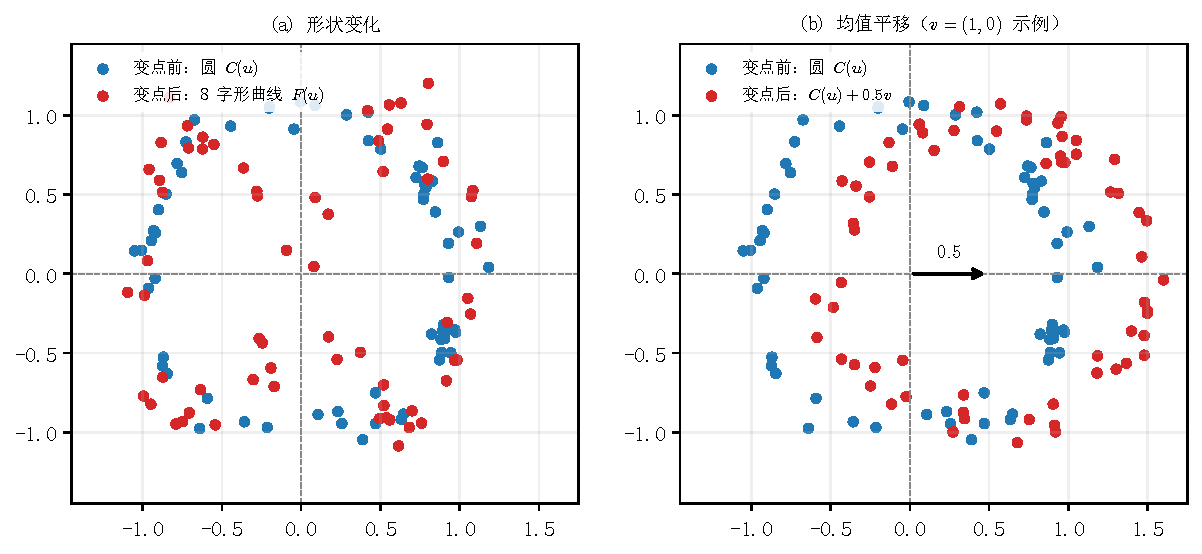
\includegraphics[width=0.95\textwidth]{../artifacts/figures/Figure2_alternative_geometry.pdf}
\caption{两类备择构造。(a) 形状变化：变点前为圆 $C(U_t)=(\cos2\pi U_t,\sin2\pi U_t)$，变点后改为 8 字形曲线 $F(U_t)=(\sin2\pi U_t,\sin4\pi U_t)$；(b) 均值平移：变点后整体平移 $+0.5v$，图中 $v=(1,0)$ 为示例方向，正式实验中 $v$ 跨重复随机、重复内固定。散点为含观测噪声 $0.08\eta_t$ 的 64 个点；圆与 8 字形曲线仅匹配单时点均值与协方差，完整滞后联合分布未被声明为相同。两个场景分别针对 BPI 与 MOMENTS 的结构敏感性。}\label{fig:alternatives}
\end{figure}

\subsection{Monte Carlo 设置}\label{sec:mc}

每格内部 $R_0=2500$（零假设）或 $R_1=1600$（备择）次主重复相互独立；不同格之间按主重复编号保留配对结构。每次方法校准均使用 $B=999$ 次内层重采样，并按式\eqref{eq:mc-pvalue}计算 $p$ 值。零假设部分包含
\[
 28\times2\text{（表示）}\times2\text{（方法）}\times2500
 =280{,}000
\]
条方法--表示评价记录；备择部分包含
\[
 2\text{（场景）}\times4\text{（条件）}\times2\text{（表示）}
 \times2\text{（方法）}\times1600
 =51{,}200
\]
条记录。外层 Monte Carlo 因而同时包含数据生成随机性与 $B=999$ 次内层校准的有限重采样随机性。

\subsection{预先设定的主对比}\label{sec:primary}

令 $\pi_{g,\rho,s,m}^{(r)}$ 表示在 BPI 表示、预算制度 $r$ 和校准方法 $m\in\{\mathrm{M0},\mathrm{M1}\}$ 下的零假设拒绝概率，且 $g\in\mathcal G=\{\mathrm{N\mbox{-}AR},\mathrm{N\mbox{-}CIRCLE}\}$。三个主对比均在确认性分析前冻结：
\begin{align}
\mathrm{P1}:\quad & D_{\mathrm{OV}}^{M}
 =\frac12\sum_{g\in\mathcal G}
 \left(\pi_{g,0,16,\mathrm{M0}}^{(M)}
      -\pi_{g,0,64,\mathrm{M0}}^{(M)}\right),
 \label{eq:p1}\\
\mathrm{P2}:\quad & D_{\mathrm{ST}}^{T}
 =\frac12\sum_{g\in\mathcal G}
 \left(\pi_{g,0,16,\mathrm{M0}}^{(T)}
      -\pi_{g,0,64,\mathrm{M0}}^{(T)}\right),
 \label{eq:p2}\\
\mathrm{P3}:\quad & D_{\mathrm{CONS}}
 =0.05-\frac12\sum_{g\in\mathcal G}
 \pi_{g,0,64,\mathrm{M1}}^{(M)}.
 \label{eq:p3}
\end{align}
P1 与 P2 检验单侧假设 $D\le0.10$ 对 $D>0.10$；P3 检验 $D_{\mathrm{CONS}}\le0.01$ 对 $D_{\mathrm{CONS}}>0.01$。阈值 $0.10$ 与 $0.01$ 均为查看确认性结果前规定的最小实质差异：$0.10$ 对应两个数据生成过程等权平均下至少 10 个百分点的 I 类错误率差异，$0.01$ 对应相对于名义水平 $0.05$ 至少 1 个百分点的保守偏差。MOMENTS 的同构对比仅作次级描述，不进入主要多重性族。

主对比使用 10,000 次按数据生成过程分层的整簇自助法。同一主重复编号下的全部相关条件、表示和方法随簇共同重采样，以保留配对结构。对一般效应量 $\widehat\theta$ 及单侧阈值 $\theta_0$，自助 $p$ 值定义为
\begin{equation}\label{eq:bootstrap-p}
 p_{\mathrm{boot}}
 =\frac{1+\sum_{b=1}^{10000}
 \mathbf1\{\widehat\theta_b^*-\widehat\theta
 \ge \widehat\theta-\theta_0\}}
 {10001}.
\end{equation}
因此，自助 $p$ 值不可能等于零。若 $q_\gamma$ 表示 10,000 个自助估计的最近秩（nearest-rank）$\gamma$ 分位数，则边际 95\% 基本型自助区间（basic bootstrap interval）\cite{DavisonHinkley1997}为
\begin{equation}\label{eq:basic-ci}
 \left[2\widehat\theta-q_{0.975},\,
       2\widehat\theta-q_{0.025}\right],
 \qquad
 q_\gamma=\widehat\theta^*_{(\lceil10000\gamma\rceil)}.
\end{equation}
三个单侧 $p$ 值采用 Holm step-down 校正\cite{Holm1979}，族水平为 $0.05$。本文将校正后 $p\le0.05$ 作为预先设定的操作性支持标准，同时用式\eqref{eq:basic-ci}报告效应量不确定性；该区间为边际区间，不解释为 Holm 同时置信区间。

\subsection{备择构造与尺寸校正功效}\label{sec:alternatives}

备择实验以 N-CIRCLE 为基础，并在完整序列上连续生成同一潜变量过程和观测噪声，不在变点处重置随机状态。令
\[
 \tau=\left\lfloor\frac T2\right\rfloor,
 \qquad
 F(u)=(\sin2\pi u,\sin4\pi u).
\]
形状变化场景定义为
\begin{equation}\label{eq:shape-alt}
 X_t=
 \begin{cases}
 C(U_t)+0.08\eta_t, & t\le\tau,\\
 F(U_t)+0.08\eta_t, & t>\tau.
 \end{cases}
\end{equation}
当 $U_t\sim U(0,1)$ 时，$C(U_t)$ 与 $F(U_t)$ 的单时点均值均为零，协方差均为 $I_2/2$；加入同分布噪声后，这两个单时点边际矩仍保持匹配。该构造不要求变点前后的完整滞后联合分布或二阶过程相同。

该备择旨在改变潜在几何中的独立循环结构，同时匹配单时点一、二阶矩：无噪声圆 $C([0,1])$ 同胚于 $S^1$，8 字形曲线 $F([0,1])$ 同胚于 $S^1\vee S^1$，二者在 $\mathbb F_2$ 系数下的一阶 Betti 数分别为 $1$ 和 $2$。但这一事实属于潜在连续曲线；有限含噪点云经 Vietoris--Rips 过滤后的持续图取决于抽样、噪声与尺度，不能被保证恰好分别产生一条与两条长寿命条带。本文实际检验的对象仍是有限点云持续图向量的均值变化。

均值平移场景定义为
\begin{equation}\label{eq:mean-alt}
 X_t=C(U_t)+0.08\eta_t+0.5v\mathbf1\{t>\tau\},
 \qquad
 v=(\cos2\pi V,\sin2\pi V),\quad V\sim U(0,1),
\end{equation}
其中方向变量 $V\sim U(0,1)$ 由独立随机流生成，与潜变量过程、观测噪声相互独立；每次 Monte Carlo 重复抽取一个方向 $v$，并在该重复内固定。每个备择场景均使用 $M=192$、$s\in\{16,64\}$ 和 $\rho\in\{0,0.8\}$，共四个条件。

尺寸校正功效使用与备择条件、表示和几何配置匹配的零假设观测统计量。将 $R_0=2500$ 个零假设统计量按升序记为
\[
 T_{M,(1)}^{H_0}\le\cdots\le T_{M,(R_0)}^{H_0},
\]
并令
\begin{equation}\label{eq:h0-critical}
 j_{0.95}=\left\lceil0.95(R_0+1)\right\rceil=2376,
 \qquad
 \widehat c_{0.95}^{H_0}=T_{M,(2376)}^{H_0}.
\end{equation}
对备择统计量 $T_{M,r}^{H_1}$，定义
\begin{equation}\label{eq:size-adjusted-power}
 \widehat\beta_{\mathrm{std}}
 =\frac1{R_1}\sum_{r=1}^{R_1}
 \mathbf1\{T_{M,r}^{H_1}>\widehat c_{0.95}^{H_0}\}.
\end{equation}
由于 M0 与 M1 共享同一观测统计量，式\eqref{eq:size-adjusted-power}在每个“条件--表示”组合上只计算一次，用于评价表示敏感性，不用于排列两种校准方法的优劣。

场景层面的表示差 $\Delta$ 通过两层整簇自助法估计。重采样单位为主复制（cluster）：零假设层按 N-CIRCLE 主复制整簇重采样以重算经验临界值，备择层按备择主复制整簇重采样以重算功效；共进行 2000 个联合 bootstrap 重复，每次分别独立重采样 H0 簇和 H1 簇，并产生一个场景差值。BPI 与 MOMENTS 使用同一重采样索引成对移动，四个 $(\rho,s)$ 条件在每个场景内先计算各自的 BPI 减 MOMENTS 功效差，再等权平均得到场景差。区间采用最近秩法（nearest-rank）定义的 2000 次百分位区间（$2.5\%$ 与 $97.5\%$ 分位数）。

\subsection{可复现性说明}\label{sec:repro}

实验协议、随机种子、配置和主要分析规则均在查看正式结果前确定。零假设与备择结果来自不可变的正式试次记录，正文数值由统一汇总文件生成。代码、环境文件、规范化结果和完整逐格输出由冻结的软件 release 提供，其地址见文末 Data and Code Availability。

\section{零假设下的有限样本校准结果}\label{sec:h0}

本节报告 28 个唯一零假设配置下，朴素置换（M0）与依赖乘子自助法（M1）的有限样本 I 类错误率。分析重点为条件化校准图谱及其逐格边界，汇总均值仅作为辅助描述。

\subsection{双预算制度下的校准图谱}\label{sec:h0-heatmap}

图~\ref{fig:m0-surface} 给出 M0 在两种预算制度下的 I 类错误率表面，图~\ref{fig:m1-deviation} 给出 M1 的校准偏差 $\widehat\alpha-0.05$。两幅图均为 $2\times2$ 分面：行区分数据生成过程，列区分固定窗口数与固定观测长度，面板内纵轴保留 $\rho$ 与步长两个条件维度。两图共有 16 个“条件--表示--方法”数值因共享几何 $s=16$、$T=3120$、$M=192$ 而被有意重复展示，用于分别解释两种预算制度，不应视为两份独立证据。完整 $16\times4$ 热图见补充材料 S4。

\begin{figure}[ht]
\centering
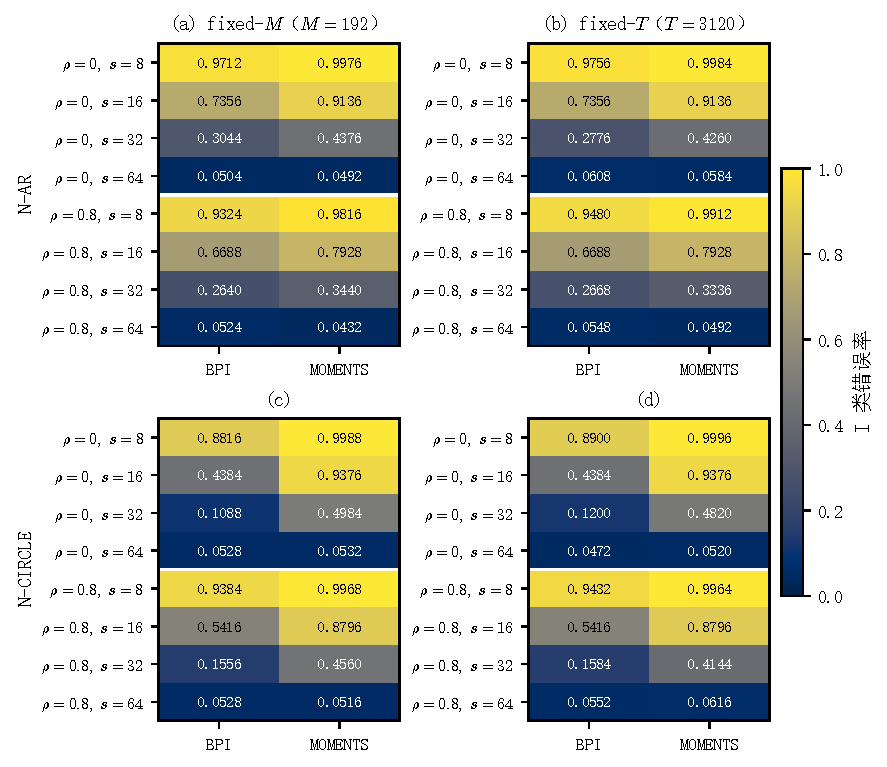
\includegraphics[width=0.92\textwidth]{../artifacts/figures/Figure3_M0_type1_surface.pdf}
\caption{M0（朴素置换）在两种预算制度下的有限样本 I 类错误率表面。两行分别为 N-AR 与 N-CIRCLE 数据生成过程，两列分别为固定窗口数（$M=192$）与固定观测长度（$T=3120$）；每面板行按 $\rho\times s$（$\rho\in\{0,0.8\}$，$s\in\{8,16,32,64\}$）排列，列为 BPI 与 MOMENTS 表示。色标 $[0,1]$，格内标注四位小数拒绝率。}\label{fig:m0-surface}
\end{figure}

\begin{figure}[ht]
\centering
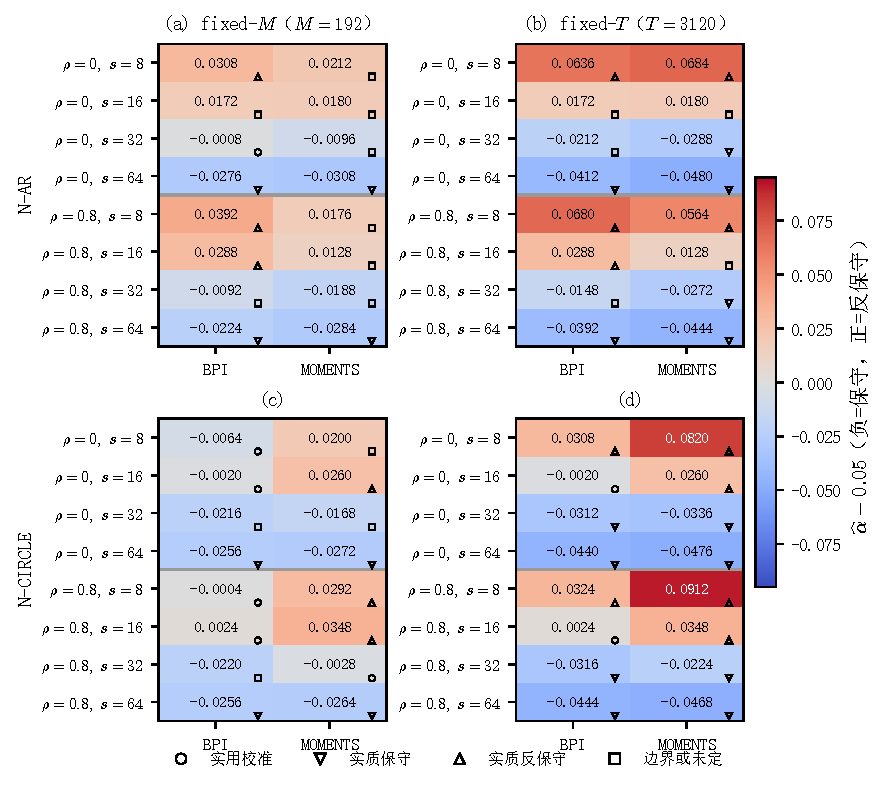
\includegraphics[width=0.92\textwidth]{../artifacts/figures/Figure4_M1_deviation_surface.pdf}
\caption{M1（依赖乘子法）在两种预算制度下的校准偏差 $\widehat\alpha-0.05$。两行分别为 N-AR 与 N-CIRCLE 数据生成过程，两列分别为固定窗口数与固定观测长度；每面板行按 $\rho\times s$（$\rho\in\{0,0.8\}$，$s\in\{8,16,32,64\}$）排列，列为 BPI 与 MOMENTS。色尺关于 0 对称，格内标注四位小数偏差；符号编码逐格 Wilson 判定（置于单元格右上角）：圆圈=实用校准，下三角=实质保守，上三角=实质反保守，方块=边界或未定。}\label{fig:m1-deviation}
\end{figure}

M0 的校准表现对窗口重叠高度敏感。BPI/M0 的逐格拒绝率介于 $0.0472$ 和 $0.9756$ 之间，MOMENTS/M0 介于 $0.0432$ 和 $0.9996$ 之间；对两种表示，20 个唯一重叠配置的 M0 均被判为实质反保守。M1 明显压缩了极端反保守性，其对应范围分别为 $0.0056$--$0.1180$ 和 $0.0020$--$0.1412$；对两种表示，8 个唯一非重叠配置的 M1 均被判为实质保守。在全部 56 个匹配的“配置--表示”组合中，M1 的拒绝率均低于 M0，但更低的拒绝率并不等同于更准确的校准。M1 的拒绝率同时分布在名义水平以下和以上，表明依赖感知乘子改变了校准图谱的形态，却未在所有有限样本配置中实现统一校准。

上述范围也说明，单一总体平均会掩盖具有相反方向的局部偏差。某些配置中的保守性和另一些配置中的反保守性可以在汇总后相互抵消，因此本文以逐格有效尺寸作为主要报告单位。

\subsection{逐格校准分类}\label{sec:h0-classify}

共有
\[
 28\text{（零假设配置）}\times2\text{（表示）}\times2\text{（方法）}=112
\]
个逐格评价单元。依据第~\ref{sec:estimands} 节的预设规则，表~\ref{tab:calibration}汇总四类校准状态。

\begin{table}[ht]
\centering
\footnotesize
\caption{逐格校准分类计数（每行 $n=28$）。完整 112 行拒绝率、Wilson 区间与分类结果见补充材料。}\label{tab:calibration}
\begin{tabular}{llcccc}
\toprule
表示 & 方法 & 实用校准 & 实质保守 & 实质反保守 & 边界/未定\\
\midrule
BPI & M0 & 7 (25.0) & 0 (0.0) & 20 (71.4) & 1 (3.6)\\
BPI & M1 & 5 (17.9) & 10 (35.7) & 7 (25.0) & 6 (21.4)\\
MOMENTS & M0 & 6 (21.4) & 0 (0.0) & 20 (71.4) & 2 (7.1)\\
MOMENTS & M1 & 1 (3.6) & 12 (42.9) & 7 (25.0) & 8 (28.6)\\
\bottomrule
\end{tabular}

\begin{minipage}{0.94\textwidth}
\vspace{0.4em}
\footnotesize 注：括号内为该类计数占 28 格的百分比。实用校准采用 90\% Wilson 区间完整落在等效带 $[0.035,0.065]$ 内，对应预设的实用等效性判据（两个单侧 5\% 判定等价于一个 90\% 双侧区间）；实质保守要求 95\% 区间完整位于实用带下方，实质反保守要求 95\% 区间完整位于实用带上方；边界/未定为既不满足实用校准、也不满足实质保守或实质反保守的剩余状态。上述计数为预设设计网格内的描述性分布，不构成方法在更广参数空间中的通过率。
\end{minipage}
\end{table}



对两种表示，M0 均有 $20/28$ 个配置被判为实质反保守，且没有配置被判为实质保守。M1 的分类则分散于实用校准、实质保守、实质反保守和边界未定四类：BPI/M1 中四类计数依次为 $5$、$10$、$7$ 和 $6$，MOMENTS/M1 中依次为 $1$、$12$、$7$ 和 $8$。这些计数描述预设设计网格内的有限样本分布，不应解释为方法在更广参数空间中的“通过率”。

\subsection{相邻格点的经验校准边界}\label{sec:h0-boundary}

题名中的“经验校准边界”对应有序设计维度上相邻格点发生校准状态变化的位置。以固定窗口数、N-AR、$\rho=0$、BPI 为例，依据逐格拒绝计数及第~\ref{sec:estimands} 节的 Wilson 判据，逐格状态随步长变化如下：$s=8,16,32$ 时 M0 均被判为实质反保守，$s=64$ 时转为实用校准，故 M0 的观测分类在步长 $32$ 与 $64$ 之间发生转换；M1 则随步长增加依次经历实质反保守（$s=8$）、边界或未定（$s=16$）、实用校准（$s=32$）与实质保守（$s=64$）。这里报告的是相邻格点的观测状态变化，不估计两点之间的连续临界步长，也不将其解释为连续参数域上的置信区间。完整的状态转换清单见补充材料 S1。

\subsection{主对比 P1--P3}\label{sec:h0-primary}

表~\ref{tab:primary}报告三个预先冻结主对比的点估计、边际 95\% basic 自助区间和 Holm 校正结果。按照第~\ref{sec:primary} 节的单侧阈值与多重性规则，三项对比均满足预设支持标准。

\begin{table}[ht]
\centering
\footnotesize
\caption{主对比 P1--P3 的效应量与推断结果。置信区间为边际 95\% basic 自助区间；原始单侧 bootstrap $p$ 值由 10,000 次整簇重采样的尾部计数按加一规则计算，随后对三项主对比实施 Holm 逐步校正，表中报告调整后 $p$ 值。}\label{tab:primary}
\begin{tabular}{llccccc}
\toprule
对比 & 估计量 & 点估计 & 阈值 & 超额效应 & 95\% basic CI & Holm $p$\\
\midrule
P1 & fixed-$M$：$s{=}16$ 减 $s{=}64$ & 0.5354 & 0.10 & 0.4354 & $[0.5210,0.5494]$ & 0.00030\\
P2 & fixed-$T$：$s{=}16$ 减 $s{=}64$ & 0.5330 & 0.10 & 0.4330 & $[0.5194,0.5462]$ & 0.00030\\
P3 & $0.05$ 减 M1 & 0.0266 & 0.01 & 0.0166 & $[0.0224,0.0308]$ & 0.00030\\
\bottomrule
\end{tabular}

\begin{minipage}{0.94\textwidth}
\vspace{0.4em}
\footnotesize 注：P1/P2 为 M0 拒绝率差（P1 固定窗口数，P2 固定观测长度），P3 为 $0.05$ 减 M1 拒绝率。三项尾部计数经真实 bootstrap 抽样核验均为 0，故原始 $p=1/10001\approx9.999\times10^{-5}$；经 Holm 逐步校正后三项调整 $p$ 均为 $3/10001\approx0.00030$。点估计与阈值之差为超额效应；正文按预设单侧阈值与多重性规则给出支持与否的表述，表中仅列统计量。
\end{minipage}
\end{table}



在固定窗口数制度下，$s=16$ 相对于 $s=64$ 的 M0 拒绝率差异，经两个数据生成过程等权平均后为 $0.5354$；在固定观测长度制度下，相应差异为 $0.5330$。两项区间的下界均远高于预设阈值 $0.10$，相对于该阈值的超额分别为 $0.4354$ 和 $0.4330$。因此，在两个预设数据生成过程、$\rho=0$ 和 BPI 表示的等权平均意义下，P1 与 P2 在各自预算制度下均超过预设的 $0.10$ 实质阈值，并通过 Holm 校正后的单侧判定。该结论不延伸为每一数据生成过程、每一依赖水平或每一表示下的必然规律。

P3 的估计为 $0.0266$，其 95\% 区间完整高于预设阈值 $0.01$。这表明在 $\rho=0$、$s=W=64$、固定 $M=192$ 的非重叠端，当前 M1 配置表现出可检测的保守偏差。该结果同时提示，依赖感知校准器在窗口不重叠时也需要接受有限样本验证。

\subsection{原序列依赖的效应修饰}\label{sec:h0-rho}

为避免将单一步长下的 $\rho$ 差异与重叠效应修饰混为一谈，次级分析采用步长对比的差。对数据生成过程 $g$、表示 $\varphi$ 和预算制度 $r$，定义
\begin{align}
 D_{g,\varphi}^{(r)}(\rho)
 &=\pi_{g,\rho,16,\mathrm{M0},\varphi}^{(r)}
  -\pi_{g,\rho,64,\mathrm{M0},\varphi}^{(r)},\\
 I_{g,\varphi}^{(r)}
 &=D_{g,\varphi}^{(r)}(0.8)-D_{g,\varphi}^{(r)}(0).
 \label{eq:rho-interaction}
\end{align}
其中 $I_{g,\varphi}^{(r)}$ 衡量原序列依赖对“$s=16$ 相对于 $s=64$”拒绝率差异的修饰。

描述性估计汇总于表~\ref{tab:rho-interaction}。正值表示 $\rho=0.8$ 放大步长对比，负值表示其缩小步长对比；修饰方向随数据生成过程和表示而变化，且不同条件的符号并不一致。由于该分析为次级描述，本文不据此提出原序列依赖具有统一单调作用的结论。

\begin{table}[ht]
\centering
\caption{原序列依赖对步长对比（$s=16$ 相对 $s=64$）的效应修饰 $I_{g,\varphi}^{(r)}$。正值表示 $\rho=0.8$ 放大步长对比，负值表示其缩小步长对比。}\label{tab:rho-interaction}
\begin{tabular}{llcc}
\toprule
表示 & 数据生成过程 & $I^{(M)}$ & $I^{(T)}$\\
\midrule
BPI & N-AR & $-0.0688$ & $-0.0608$\\
BPI & N-CIRCLE & $0.1032$ & $0.0952$\\
MOMENTS & N-AR & $-0.1148$ & $-0.1116$\\
MOMENTS & N-CIRCLE & $-0.0564$ & $-0.0676$\\
\bottomrule
\end{tabular}
\end{table}

\section{表示特异性的检出与定位性能}\label{sec:h1}

本节考察两类方向相反的备择。尺寸标准化功效按式\eqref{eq:size-standardized-power}计算：每个备择条件和表示均使用对应零假设配置的经验 0.95 临界值，从而减少参考分布松紧对表示比较的直接干扰。由于 M0 与 M1 使用相同的观测扫描统计量，每个“条件--表示”组合只产生一个尺寸标准化功效。场景层面的功效为四个预设条件 $(\rho,s)\in\{0,0.8\}\times\{16,64\}$ 的等权平均。

\subsection{形状变化}\label{sec:h1-shape}

在圆形到八字曲线的形状变化下，两种表示的平均尺寸标准化功效分别为
\[
 \widehat\beta_{\mathrm{BPI}}=1.00000,
 \qquad
 \widehat\beta_{\mathrm{MOMENTS}}=0.06203.
\]
定义场景差异为 BPI 减去 MOMENTS，则
\begin{equation}\label{eq:shape-power-diff}
 \Delta_{\mathrm{shape}}=0.93797,
 \qquad
 \text{95\% CI }[0.92969,0.94609].
\end{equation}
该区间为 2000 次保持条件配对结构的重采样所得 95\% 百分位自助区间。结果表明，在当前形状构造和固定表示参数下，BPI 保留了 MOMENTS 的一、二阶摘要未充分捕获的结构信息。该证据的适用范围限于本文定义的备择、窗口几何和表示实现，不能推广为拓扑表示对任意变化类型均占优势。

\subsection{均值平移反向对照}\label{sec:h1-mean}

在均值平移场景下，BPI 的平均尺寸标准化功效为 $0.05375$，MOMENTS 为 $1.00000$，因此
\begin{equation}\label{eq:mean-power-diff}
 \Delta_{\mathrm{mean}}=-0.94625,
 \qquad
 \text{95\% CI }[-0.95344,-0.93844].
\end{equation}
差异方向与形状变化场景相反。MOMENTS 直接包含窗口均值，因而在该构造中具有很高的检出能力；BPI 的尺寸标准化功效接近名义水平，说明固定持续强度表示对该平移信号的敏感性有限。

\begin{figure}[ht]
\centering
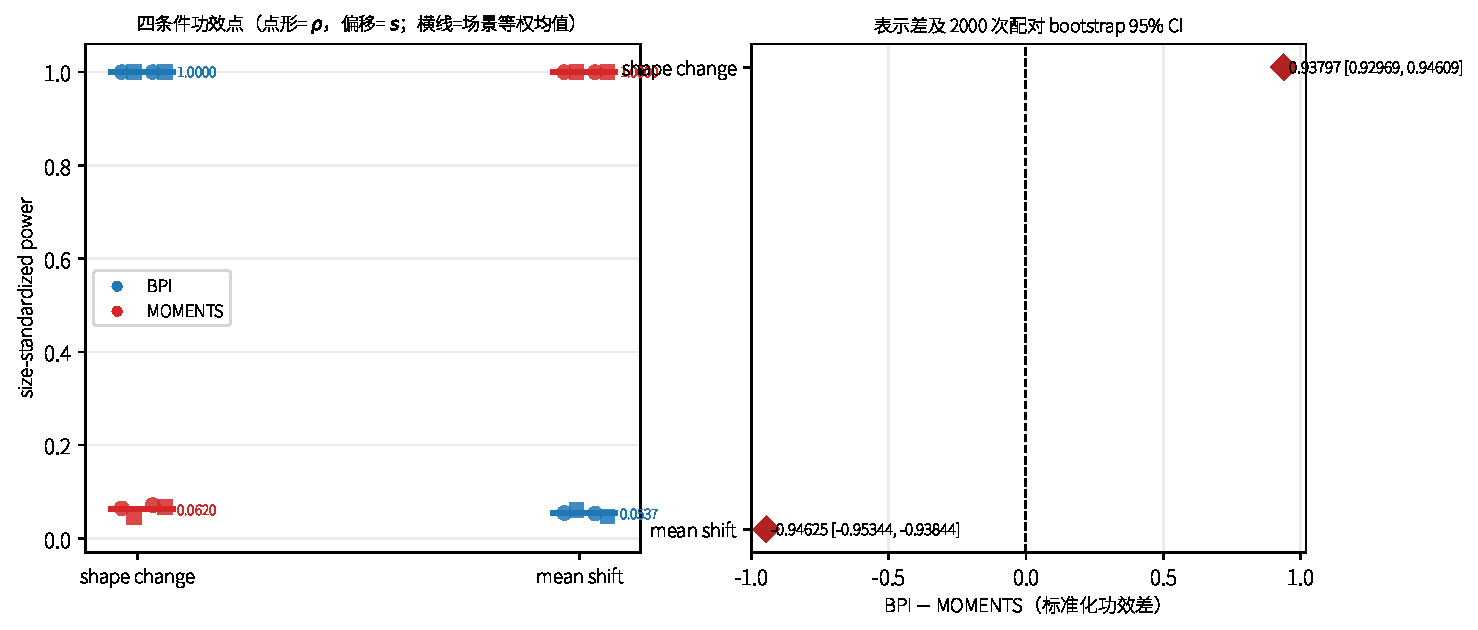
\includegraphics[width=0.95\textwidth]{../artifacts/figures/Figure5_H1_power_and_difference.pdf}
\caption{左：形状变化与均值平移下 BPI 与 MOMENTS 的条件级尺寸标准化功效。小点为四个预设条件之一（点形编码 $\rho$：圆圈 $\rho=0$，方块 $\rho=0.8$；水平偏移编码 $s$）；横线为场景等权平均功效。两个场景之间不使用连线，以避免暗示连续变化趋势。右：两个场景下 BPI 减去 MOMENTS 的功效差及 2000 次配对百分位自助 95\% 区间，零线表示无差异。右图区间只对应表示差异，不用作单个表示功效均值的误差条。完整 16 行条件级结果见补充材料。}\label{fig:h1-power}
\end{figure}

两个场景中出现的样本功效 $1.00000$ 表示 1600 次有限 Monte Carlo 重复在全部四个条件上的汇总结果，未构成总体功效恒等于 1 的概率保证。式\eqref{eq:shape-power-diff}与式\eqref{eq:mean-power-diff}共同支持表示选择性的结论：拓扑表示和矩表示保留了不同类型的变化信息，任何单一表示的检出能力均应结合备择结构加以评价。

\subsection{名义功效与尺寸标准化功效}\label{sec:h1-std}

直接以 $p\le0.05$ 计算的名义功效同时受到观测统计量和校准参考分布的影响。当对应零假设配置未达到点态实用校准时，名义功效可能因反保守性而被抬高，也可能因保守性而被压低。尺寸标准化功效改用匹配零假设统计量的经验临界值，使 BPI 与 MOMENTS 在各自零假设尺度上接受比较。该指标仍是条件化的有限样本量，不能消除表示维数、窗口参数和备择强度等设计因素的影响。

\subsection{定位误差与联合成功率}\label{sec:h1-localization}

位置估计由观测扫描曲线确定，按式\eqref{eq:location-map}映射回原始时间轴。由于变化在 $t=\lfloor T/2\rfloor$ 与 $t=\lfloor T/2\rfloor+1$ 之间发生，真实连续边界为
\begin{equation}\label{eq:true-location}
 \tau_{\mathrm{true}}=\left\lfloor\frac T2\right\rfloor+\frac12.
\end{equation}
本文报告无条件绝对误差
\[
 E_r=|\widehat\tau_r-\tau_{\mathrm{true}}|,
\]
原始尺度平均绝对误差 $R_1^{-1}\sum_rE_r$，以及归一化平均绝对误差
\begin{equation}\label{eq:normalized-mae}
 \operatorname{nMAE}
 =\frac1{R_1}\sum_{r=1}^{R_1}\frac{E_r}{T}.
\end{equation}
位置误差由观测统计量决定，因此对同一“条件--表示”组合，M0 与 M1 共享相同的 $\widehat\tau_r$。校准方法只通过拒绝事件影响联合成功率。对方法 $m\in\{\mathrm{M0},\mathrm{M1}\}$，定义
\begin{equation}\label{eq:joint-success}
 \widehat J_m
 =\frac1{R_1}\sum_{r=1}^{R_1}
 \mathbf1\left\{p_{r,m}\le0.05,\;
 |\widehat\tau_r-\tau_{\mathrm{true}}|\le\frac W2\right\}.
\end{equation}
漏检重复保留在式\eqref{eq:joint-success}的分母中，因此该量同时评价检出与定位。

表~\ref{tab:h1-power}以同一场景内四个预设条件的等权平均汇总功效、归一化定位误差和联合成功率。不同步长对应的 $T$ 不同，故正文采用式\eqref{eq:normalized-mae}保证条件间尺度可比；逐条件原始 MAE、匹配零假设临界值和对应 I 类错误率见补充材料。定位汇总由既有观测扫描结果重新计算，未改变或重跑 Monte Carlo 试次。

\begin{table}[ht]
\centering
\caption{同一场景内四个预设条件的等权描述性汇总。尺寸标准化功效使用各自匹配的零假设临界值；平均归一化 MAE 为无条件位置误差除以对应 $T$ 后的均值；联合成功率按式\eqref{eq:joint-success}分别计算。}\label{tab:h1-power}
\begingroup
\footnotesize
\setlength{\tabcolsep}{3.5pt}
\begin{tabular}{llccrr}
\toprule
场景 & 表示 & 检出能力 & 定位误差 & \multicolumn{2}{c}{检出--定位联合成功}\\
\cmidrule(lr){3-3}\cmidrule(lr){4-4}\cmidrule(lr){5-6}
 & & $\widehat\beta_{\mathrm{std}}$ & nMAE & M0 & M1\\
\midrule
形状变化 & BPI & 1.00000 & 0.00409 & 0.9839 & 0.9839\\
形状变化 & MOMENTS & 0.06203 & 0.20165 & 0.0144 & 0.0009\\
均值平移 & BPI & 0.05375 & 0.20255 & 0.0087 & 0.0011\\
均值平移 & MOMENTS & 1.00000 & 0.00330 & 0.9052 & 0.9052\\
\bottomrule
\end{tabular}
\endgroup
\end{table}



% 本稿未纳入自然数据案例；外部验证边界在讨论部分明确说明。

\section{讨论}\label{sec:discussion}

\subsection{重叠窗口引起的随机化单位错配}\label{sec:disc-validity}

本文的理论和模拟共同表明，重叠窗口带来的推断问题超出了“相关样本使有效样本量下降”的标量解释范围。窗口重用首先改变派生特征的联合分布：即使原始观测独立同分布，相邻特征仍可能共享大量底层随机变量，并形成随窗口距离变化的协方差。全局随机置换操作保留经验边际分布，却打散原始顺序中的滞后协方差，因此科学零假设下的“无变化”无法自动提供窗口层面的排列不变性。命题~\ref{prop:counterexample}给出了这一层级错配的有限样本反例，式\eqref{eq:permutation-fpc}则说明排列参考的条件变异只由经验边际量决定。该机制与依赖时间序列中置换检验需要附加有效性条件的既有理论一致\cite{RomanoTirlea2022}。

有效样本量仍可作为特定线性统计量的直观概括。例如，$W=64$、$s=16$、$M=192$ 时，窗口均值的方差比约为 $3.974$。然而，窗口均值的方差比可以解释特定线性统计量的变异变化，但不能直接决定一般高维最大扫描的参考分布及其拒绝率。本文因此对完整检验逐条件开展模拟评价。

\subsection{双预算视角与条件化校准图谱}\label{sec:disc-surface}

固定窗口数和固定观测长度回答不同的条件问题。前者保持扫描序列长度 $M$ 不变，步长变化同时改变原始观测长度；后者保持 $T$ 不变，步长变化同时改变窗口数。两种制度均无法单独隔离所有设计因素，但它们提供了互补的预算视角。P1 与 P2 在两个预设数据生成过程的等权平均下均超过预设实质阈值，说明严重失校准并非某一种预算制度的偶然产物。相应结论仍应限定于本文的 $W$、步长网格、数据生成过程和表示实现。

校准图谱的概念还强调，汇总平均不能替代逐格有效性判断。朴素置换下，BPI 与 MOMENTS 的拒绝率范围分别为 $0.0472$--$0.9756$ 和 $0.0432$--$0.9996$。依赖乘子校准下，相应范围分别为 $0.0056$--$0.1180$ 和 $0.0020$--$0.1412$。将条件间的保守性与反保守性合并，可能得到接近 $0.05$ 的总体均值，同时掩盖局部严重失真。因此，本文将逐格拒绝率、Wilson 区间和预设实用等价带作为主要证据。该分类依赖 Monte Carlo 样本量和等价带宽度，属于操作性有限样本判据。

\subsection{依赖乘子校准的改善与局限}\label{sec:disc-dmb}

M1 在多数重叠配置中大幅降低了 M0 的极端反保守性，说明相关乘子在参考过程中引入了预设相关结构。不过，M1 仍同时产生实质保守和实质反保守配置。一般 dependent wild bootstrap 或依赖乘子理论主要针对特定均值、光滑函数或经验过程\cite{Shao2010,BucherKojadinovic2016}：Shao 的 dependent wild bootstrap 面向平稳序列的部分和近似，B{\"u}cher 与 Kojadinovic 的依赖乘子则针对强混合经验 copula 过程，二者均在各自函数类内给出渐近有效性。这些理论为窗口特征序列提供了渐近分析的起点，但均未提供本文完整 BPI 最大扫描在当前样本规模和固定带宽规则下的有限样本校准保证；其适用性仍需针对本文的局部映射、扫描泛函与带宽规则逐项验证。

当前带宽规则也有助于解释非重叠端的保守性。即使 $s=W$，式\eqref{eq:dmb-bandwidth}中的 $\lceil M^{1/3}\rceil$ 仍使 $b>1$；以 P3 的固定 $M=192$ 配置为例，$b=6$，相关乘子不会退化为独立乘子。P3 检出的保守偏差与这一结构相容，但本文没有进一步分解带宽、桥接和高维特征谱各自的贡献。后续研究可针对窗口依赖尺度推导步长适配的乘子协方差，或在原始时间轴上实施块重采样并重新构造全部窗口特征。此类扩展需要新的理论和独立确认实验。

\subsection{表示敏感性与校准有效性}\label{sec:disc-representation}

形状变化和均值平移中的功效反转说明，表示选择决定了观测统计量能够保留何种信号。BPI 在圆形到 8 字形曲线的变化中具有很高的尺寸校正功效，MOMENTS 在均值平移中具有对应优势。尺寸校正临界值减少了零假设校准松紧对这一比较的直接影响，因此结果更接近表示层面的信号选择性。与此同时，该比较仍受窗口宽度、表示超参数、变化强度和有限样本设计约束。

表示敏感性与校准有效性应作为两个不同评价维度。信息不足的表示难以通过更准确的校准获得高功效；失真的参考分布也会使信息充分的表示产生错误的显著性判断。两者在有限样本下还可能通过维数、依赖谱和乘子带宽发生交互，本文没有假设其统计独立或严格正交。定位结果进一步显示，观测扫描曲线决定无条件位置误差，校准方法通过拒绝事件影响“检出且定位成功”的联合概率；这两个指标回答的统计问题需要保持区分。

\subsection{实践含义}\label{sec:disc-practice}

对采用重叠窗口的拓扑变化检测，本文给出三条操作建议：\begin{enumerate}\item 将窗口视为派生统计单位，而非因原始观测独立同分布就直接实施窗口级全局随机置换；校准单位应显式声明。\item 方法报告应明确窗口宽度、步长、原始长度、窗口数与校准单位，并在与实际管线匹配的零假设下逐条件评估 I 类错误率，而非依赖单一汇总平均。\item 固定观测预算与固定窗口数对应不同部署约束，其结论不宜互相替代；依赖感知重采样可作为更合理的参考起点，但其带宽与有限样本行为仍需针对具体表示与扫描统计量验证。\end{enumerate}

\subsection{研究局限}\label{sec:limitations}

本文的结论具有以下局限。
\begin{enumerate}
\item BPI 网格、核宽、尺度上界、同调通道和 MOMENTS 构造均保持固定；本文未系统遍历表示超参数，也未研究特征维数与校准行为之间的敏感性。
\item 零假设仅包含 N-AR 与 N-CIRCLE 两类合成过程，主要结论依赖两个过程的等权设计；更广的非高斯、长记忆、异方差和非平稳零模型尚待检验。
\item 备择仅包括一种形状变化和一种均值平移。形状构造匹配单时点边际均值与协方差，但没有匹配完整滞后联合分布或二阶过程。
\item M1 是冻结的依赖感知参考方法，本文没有为完整 BPI 最大扫描建立新的有限样本或渐近有效性定理，当前带宽规则也未针对每个步长进行最优选择。
\item 逐格校准分类为点态判断，依赖预设等价带和 Monte Carlo 精度，不提供整个设计域上的同时保证。
\item 本稿未纳入自然数据或独立外部数据集，外部有效性主要由合成设计的覆盖范围限定。
\item 本文研究单一变点的最大扫描，尚未处理多变点递归、停止规则及相应的族错误率控制。
\end{enumerate}

\section{结论}\label{sec:conclusion}

本文评估了基于持续同调特征的变点检验在重叠滑动窗口下的有限样本校准。窗口均值反例说明，原始观测独立同分布不能自动保证派生窗口序列具有交换性。在所考察的设计网格内，朴素置换在两种表示的全部重叠配置中均表现为实质反保守；依赖乘子法普遍降低拒绝率，但在非重叠配置中表现为实质保守，未实现逐条件统一校准。原序列依赖对步长对比的影响随数据生成过程和表示变化。形状备择和整体平移负对照进一步表明，持续同调表示保留的结构信息及其不变性，需要与下游检验的误报控制分开解释。上述结论为当前固定实现提供有限样本参照，其范围由生成过程、窗口设计、表示参数和校准规则共同限定。


\section*{Data and Code Availability}
复现本文结果的代码、配置、种子清单、完整逐格数据与补充材料由仓库 \url{https://github.com/dw0911/owtda-calibration} 提供。本稿对应 git 标签 \texttt{v1.1.1-paper}；全部合成数据均由该版本代码与固定随机种子生成，不依赖外部数据归档，独立数据 DOI 尚在建立中，未作为已提供材料列出。补充材料 S5 给出代码入口与复现步骤。

\bibliographystyle{unsrt}
\bibliography{bibliography}
\end{document}
